%**************************************%
%* Generated from MathBook XML source *%
%*    on 2017-05-29T10:09:10-06:00    *%
%*                                    *%
%*   http://mathbook.pugetsound.edu   *%
%*                                    *%
%**************************************%
\documentclass[10pt,]{book}
%% Custom Preamble Entries, early (use latex.preamble.early)
%% Inline math delimiters, \(, \), need to be robust
%% 2016-01-31:  latexrelease.sty  supersedes  fixltx2e.sty
%% If  latexrelease.sty  exists, bugfix is in kernel
%% If not, bugfix is in  fixltx2e.sty
%% See:  https://tug.org/TUGboat/tb36-3/tb114ltnews22.pdf
%% and read "Fewer fragile commands" in distribution's  latexchanges.pdf
\IfFileExists{latexrelease.sty}{}{\usepackage{fixltx2e}}
%% Text height identically 9 inches, text width varies on point size
%% See Bringhurst 2.1.1 on measure for recommendations
%% 75 characters per line (count spaces, punctuation) is target
%% which is the upper limit of Bringhurst's recommendations
%% Load geometry package to allow page margin adjustments
\usepackage{geometry}
\geometry{letterpaper,total={340pt,9.0in}}
%% Custom Page Layout Adjustments (use latex.geometry)
\geometry{papersize={6in,9in}, hmargin={0.85in, 0.5in}, height=7.75in, top=0.75in, twoside, ignoreheadfoot}
%% This LaTeX file may be compiled with pdflatex, xelatex, or lualatex
%% The following provides engine-specific capabilities
%% Generally, xelatex and lualatex will do better languages other than US English
%% You can pick from the conditional if you will only ever use one engine
\usepackage{ifthen}
\usepackage{ifxetex,ifluatex}
\ifthenelse{\boolean{xetex} \or \boolean{luatex}}{%
%% begin: xelatex and lualatex-specific configuration
%% fontspec package will make Latin Modern (lmodern) the default font
\ifxetex\usepackage{xltxtra}\fi
\usepackage{fontspec}
%% realscripts is the only part of xltxtra relevant to lualatex 
\ifluatex\usepackage{realscripts}\fi
%% 
%% Extensive support for other languages
\usepackage{polyglossia}
%% Main document language is US English
\setdefaultlanguage{english}
%% Spanish
\setotherlanguage{spanish}
%% Vietnamese
\setotherlanguage{vietnamese}
%% end: xelatex and lualatex-specific configuration
}{%
%% begin: pdflatex-specific configuration
%% translate common Unicode to their LaTeX equivalents
%% Also, fontenc with T1 makes CM-Super the default font
%% (\input{ix-utf8enc.dfu} from the "inputenx" package is possible addition (broken?)
\usepackage[T1]{fontenc}
\usepackage[utf8]{inputenc}
%% end: pdflatex-specific configuration
}
%% Symbols, align environment, bracket-matrix
\usepackage{amsmath}
\usepackage{amssymb}
%% allow page breaks within display mathematics anywhere
%% level 4 is maximally permissive
%% this is exactly the opposite of AMSmath package philosophy
%% there are per-display, and per-equation options to control this
%% split, aligned, gathered, and alignedat are not affected
\allowdisplaybreaks[4]
%% allow more columns to a matrix
%% can make this even bigger by overriding with  latex.preamble.late  processing option
\setcounter{MaxMatrixCols}{30}
%%
%% Color support, xcolor package
%% Always loaded.  Used for:
%% mdframed boxes, add/delete text, author tools
\PassOptionsToPackage{usenames,dvipsnames,svgnames,table}{xcolor}
\usepackage{xcolor}
%%
%% Semantic Macros
%% To preserve meaning in a LaTeX file
%% Only defined here if required in this document
%% Used for inline definitions of terms
\newcommand{\terminology}[1]{\textbf{#1}}
%% Subdivision Numbering, Chapters, Sections, Subsections, etc
%% Subdivision numbers may be turned off at some level ("depth")
%% A section *always* has depth 1, contrary to us counting from the document root
%% The latex default is 3.  If a larger number is present here, then
%% removing this command may make some cross-references ambiguous
%% The precursor variable $numbering-maxlevel is checked for consistency in the common XSL file
\setcounter{secnumdepth}{1}
%% Environments with amsthm package
%% Theorem-like environments in "plain" style, with or without proof
\usepackage{amsthm}
\theoremstyle{plain}
%% Numbering for Theorems, Conjectures, Examples, Figures, etc
%% Controlled by  numbering.theorems.level  processing parameter
%% Always need a theorem environment to set base numbering scheme
%% even if document has no theorems (but has other environments)
\newtheorem{theorem}{Theorem}[section]
%% Only variants actually used in document appear here
%% Style is like a theorem, and for statements without proofs
%% Numbering: all theorem-like numbered consecutively
%% i.e. Corollary 4.3 follows Theorem 4.2
\newtheorem{corollary}[theorem]{Corollary}
%% Numbering for Projects (independent of others)
%% Controlled by  numbering.projects.level  processing parameter
%% Always need a project environment to set base numbering scheme
%% even if document has no projectss (but has other blocks)
\newtheorem{project}{Project}%% Project-like environments, normal text
\theoremstyle{definition}
\newtheorem{activity}[project]{Activity}
\newtheorem{task}[project]{Task}
%% Localize LaTeX supplied names (possibly none)
\renewcommand*{\chaptername}{Chapter}
%% Equation Numbering
%% Controlled by  numbering.equations.level  processing parameter
\numberwithin{equation}{chapter}
%% For improved tables
\usepackage{array}
%% Some extra height on each row is desirable, especially with horizontal rules
%% Increment determined experimentally
\setlength{\extrarowheight}{0.2ex}
%% Define variable thickness horizontal rules, full and partial
%% Thicknesses are 0.03, 0.05, 0.08 in the  booktabs  package
\makeatletter
\newcommand{\hrulethin}  {\noalign{\hrule height 0.04em}}
\newcommand{\hrulemedium}{\noalign{\hrule height 0.07em}}
\newcommand{\hrulethick} {\noalign{\hrule height 0.11em}}
%% We preserve a copy of the \setlength package before other
%% packages (extpfeil) get a chance to load packages that redefine it
\let\oldsetlength\setlength
\newlength{\Oldarrayrulewidth}
\newcommand{\crulethin}[1]%
{\noalign{\global\oldsetlength{\Oldarrayrulewidth}{\arrayrulewidth}}%
\noalign{\global\oldsetlength{\arrayrulewidth}{0.04em}}\cline{#1}%
\noalign{\global\oldsetlength{\arrayrulewidth}{\Oldarrayrulewidth}}}%
\newcommand{\crulemedium}[1]%
{\noalign{\global\oldsetlength{\Oldarrayrulewidth}{\arrayrulewidth}}%
\noalign{\global\oldsetlength{\arrayrulewidth}{0.07em}}\cline{#1}%
\noalign{\global\oldsetlength{\arrayrulewidth}{\Oldarrayrulewidth}}}
\newcommand{\crulethick}[1]%
{\noalign{\global\oldsetlength{\Oldarrayrulewidth}{\arrayrulewidth}}%
\noalign{\global\oldsetlength{\arrayrulewidth}{0.11em}}\cline{#1}%
\noalign{\global\oldsetlength{\arrayrulewidth}{\Oldarrayrulewidth}}}
%% Single letter column specifiers defined via array package
\newcolumntype{A}{!{\vrule width 0.04em}}
\newcolumntype{B}{!{\vrule width 0.07em}}
\newcolumntype{C}{!{\vrule width 0.11em}}
\makeatother
%% Figures, Tables, Listings, Floats
%% The [H]ere option of the float package fixes floats in-place,
%% in deference to web usage, where floats are totally irrelevant
%% We re/define the figure, table and listing environments, if used
%%   1) New mbxfigure and/or mbxtable environments are defined with float package
%%   2) Standard LaTeX environments redefined to use new environments
%%   3) Standard LaTeX environments redefined to step theorem counter
%%   4) Counter for new environments is set to the theorem counter before caption
%% You can remove all this figure/table setup, to restore standard LaTeX behavior
%% HOWEVER, numbering of figures/tables AND theorems/examples/remarks, etc
%% WILL ALL de-synchronize with the numbering in the HTML version
%% You can remove the [H] argument of the \newfloat command, to allow flotation and 
%% preserve numbering, BUT the numbering may then appear "out-of-order"
\usepackage{float}
\usepackage[bf]{caption} % http://tex.stackexchange.com/questions/95631/defining-a-new-type-of-floating-environment 
\usepackage{newfloat}
% Figure environment setup so that it no longer floats
\SetupFloatingEnvironment{figure}{fileext=lof,placement={H},within=section,name=Figure}
% figures have the same number as theorems: http://tex.stackexchange.com/questions/16195/how-to-make-equations-figures-and-theorems-use-the-same-numbering-scheme 
\makeatletter
\let\c@figure\c@theorem
\makeatother
% Table environment setup so that it no longer floats
\SetupFloatingEnvironment{table}{fileext=lot,placement={H},within=section,name=Table}
% tables have the same number as theorems: http://tex.stackexchange.com/questions/16195/how-to-make-equations-figures-and-theorems-use-the-same-numbering-scheme 
\makeatletter
\let\c@table\c@theorem
\makeatother
%% Footnote Numbering
%% We reset the footnote counter, as given by numbering.footnotes.level
\makeatletter\@addtoreset{footnote}{chapter}\makeatother
%% Raster graphics inclusion, wrapped figures in paragraphs
%% \resizebox sometimes used for images in side-by-side layout
\usepackage{graphicx}
%%
%% More flexible list management, esp. for references and exercises
%% But also for specifying labels (i.e. custom order) on nested lists
\usepackage{enumitem}
%% Lists of references in their own section, maximum depth 1
\newlist{referencelist}{description}{4}
\setlist[referencelist]{leftmargin=!,labelwidth=!,labelsep=0ex,itemsep=1.0ex,topsep=1.0ex,partopsep=0pt,parsep=0pt}
%% Support for index creation
%% imakeidx package does not require extra pass (as with makeidx)
%% Title of the "Index" section set via a keyword
%% Language support for the "see" and "see also" phrases
\usepackage{imakeidx}
\makeindex[title=Index, intoc=true]
\renewcommand{\seename}{see}
\renewcommand{\alsoname}{see also}
%% hyperref driver does not need to be specified, it will be detected
\usepackage{hyperref}
%% Hyperlinking active in PDFs, all links solid and blue
\hypersetup{colorlinks=true,linkcolor=blue,citecolor=blue,filecolor=blue,urlcolor=blue}
\hypersetup{pdftitle={Combinatorics Through Guided Discovery}}
%% If you manually remove hyperref, leave in this next command
\providecommand\phantomsection{}
%% Graphics Preamble Entries
\usepackage{tikz}
\usepackage{tkz-graph}
\usepackage{tkz-euclide}
\usetikzlibrary{patterns}
\usetikzlibrary{positioning}
\usetikzlibrary{matrix,arrows}
\usetikzlibrary{calc}
\usetikzlibrary{shapes}
\usetikzlibrary{through,intersections,decorations,shadows,fadings}

\usepackage{pgfplots}
%% If tikz has been loaded, replace ampersand with \amp macro
%% extpfeil package for certain extensible arrows,
%% as also provided by MathJax extension of the same name
%% NB: this package loads mtools, which loads calc, which redefines
%%     \setlength, so it can be removed if it seems to be in the 
%%     way and your math does not use:
%%     
%%     \xtwoheadrightarrow, \xtwoheadleftarrow, \xmapsto, \xlongequal, \xtofrom
%%     
%%     we have had to be extra careful with variable thickness
%%     lines in tables, and so also load this package late
\usepackage{extpfeil}
%% Custom Preamble Entries, late (use latex.preamble.late)
%% Begin: Author-provided packages
%% (From  docinfo/latex-preamble/package  elements)
%% End: Author-provided packages
%% Begin: Author-provided macros
%% (From  docinfo/macros  element)
%% Plus three from MBX for XML characters
\newcommand{\cycle}[1]{\arraycolsep 5 pt
\left(\begin{array}#1\end{array}\right)}
\newcommand{\iteme}{
\item[\ $\bullet$\ \theenumi.]}
\newcommand{\items}{
\item[\ \tiny$+$\ \theenumi.]}
\newcommand{\itemh}{
\item[\ {$*$}\ \theenumi.]}
\newcommand{\itemes}{
\item[\ \Large$\cdot$\ \theenumi.]}
\newcommand{\itemesi}{
 \item[\ \importantarrow\ \Large
$\cdot$\ \theenumi.]}
\newcommand{\itemm}{
\item[\ $\circ$\ \theenumi.]}
\newcommand{\importantarrow}{$\Rightarrow$}
\newcommand{\itemi}{
\item[\ \importantarrow\ \theenumi.]}
\newcommand{\itemitemi}{
\item[\ \importantarrow\ (\theenumii)]}
\newcommand{\itemei}{
\item[\ \importantarrow\ $\bullet$\ \theenumi.]}
\newcommand{\itemih}{
\item[\ \importantarrow\ $*$\ \theenumi.]}
\newcommand{\itemitemih}{
\item[\ \importantarrow\ $*$\ (\theenumii)]}
\newcommand{\itemitemh}{
\item[\ $*$\ (\theenumii)]}
\newcommand{\qchoose}[2]{\left[{#1\atop#2}\right]_q}
\def\neg1choose#1#2{\left[{#1\atop#2}\right]_{-1}}
\newcommand{\bp}{
\begin{enumerate}{\setcounter{enumi}{\value{problemnumber}}}}
\newcommand{\ep}{\setcounter{problemnumber}{\value{enumi}}
\end{enumerate}}
\newcommand{\ignore}[1]{}
\renewcommand{\bottomfraction}{.8}
\renewcommand{\topfraction}{.8}
\newcommand{\apple}{\mbox{A}}
\newcommand{\ap}{\apple}
\newcommand{\banana}{\mbox{B}}
\newcommand{\ba}{\banana}
\newcommand{\pear}{\mbox{P}}
\newcommand{\pe}{\pear}
\newcommand{\lt}{<}
\newcommand{\gt}{>}
\newcommand{\amp}{&}
%% End: Author-provided macros
%% Title page information for book
\title{Combinatorics Through Guided Discovery}
\author{Kenneth P. Bogart
}
\date{}
\begin{document}
\frontmatter
%% no half-title
%% No adcard
%% begin: title page
%% Inspired by Peter Wilson's "titleDB" in "titlepages" CTAN package
\thispagestyle{empty}
{\centering
\vspace*{0.14\textheight}
%% Target for xref to top-level element is ToC
\addtocontents{toc}{\protect\hypertarget{index}{}}
{\Huge Combinatorics Through Guided Discovery}\\[3\baselineskip]
{\Large Kenneth P. Bogart}\\}
\clearpage
%% end:   title page
%% begin: copyright-page
\thispagestyle{empty}
\vspace*{\stretch{2}}
\vspace*{\stretch{1}}
\null\clearpage
%% end:   copyright-page
%% begin: preface
\chapter*{Preface}\label{preface-1}
\addcontentsline{toc}{chapter}{Preface}
This book is an introduction to combinatorial mathematics, also known as combinatorics. The book focuses especially but not exclusively on the part of combinatorics that mathematicians refer to as ``counting.'' The book consist almost entirely of problems.  Some of the problems are designed to lead you to think about a concept, others are designed to help you figure out a concept and state a theorem about it, while still others ask you to prove the theorem. Other problems give you a chance to use a theorem you have proved. From time to time there is a discussion that pulls together some of the things you have learned or introduces a new idea for you to work with. Many of the problems are designed to build up your intuition for how combinatorial mathematics works. There are problems that some people will solve quickly, and there are problems that will take days of thought for everyone. Probably the best way to use this book is to work on a problem until you feel you are not making progress and then go on to the next one. Think about the problem you couldn't get as you do other things. The next chance you get, discuss the problem you are stymied on with other members of the class. Often you will all feel you've hit dead ends, but when you begin comparing notes and listening \emph{carefully} to each other, you will see more than one approach to the problem and be able to make some progress. In fact, after comparing notes you may realize that there is more than one way to interpret the problem. In this case your first step should be to think together about what the problem is actually asking you to do. You may have learned in school that for every problem you are given, there is a method that has already been taught to you, and you are supposed to figure out which method applies and apply it. That is not the case here.  Based on some simplified examples, you will discover the method for yourself. Later on, you may recognize a pattern that suggests you should try to use this method again.%
\par
The point of learning from this book is that you are learning how to discover ideas and methods for yourself, not that you are learning to apply methods that someone else has told you about. The problems in this book are designed to lead you to discover for yourself and prove for yourself the main ideas of combinatorial mathematics.  There is considerable evidence that this leads to deeper learning and more understanding.%
\par
You will see that some of the problems are marked with bullets. Those are the problems that I feel are essential to having an understanding of what comes later, whether or not it is marked by a bullet. The problems with bullets are the problems in which the main ideas of the book are developed. Your instructor may leave out some of these problems because he or she plans not to cover future problems that rely on them. Many problems, in fact entire sections, are not marked in this way, because they use an important idea rather than developing one. Some other special symbols are described in what follows; a summary appears in \hyperref[tab_prob-symbs-pref]{Table~\ref{tab_prob-symbs-pref}}.%
\begin{table}
\centering
\begin{tabular}{ll}
&\tabularnewline\hrulethin
\(\bullet\)&essential\tabularnewline[0pt]
\(\circ\)&motivational material\tabularnewline[0pt]
\(+\)&summary\tabularnewline[0pt]
\importantarrow&especially interesting\tabularnewline[0pt]
\(*\)&difficult\tabularnewline[0pt]
\(\cdot\)&essential for this section or the next\tabularnewline[0pt]
&\tabularnewline\hrulethin
\end{tabular}
\caption{The meaning of the symbols to the left of problem numbers.\label{tab_prob-symbs-pref}}
\end{table}
Some problems are marked with open circles. This indicates that they are designed to provide motivation for, or an introduction to, the important concepts, motivation with which some students may already be familiar. You will also see that some problems are marked with arrows. These point to problems that I think are particularly interesting. Some of them are also difficult, but not all are. A few problems that summarize ideas that have come before but aren't really essential are marked with a plus, and problems that are essential if you want to cover the section they are in or, perhaps, the next section, are marked with a dot (a small bullet). If a problem is relevant to a much later section in an essential way, I've marked it with a dot and a parenthetical note that explains where it will be essential. Finally, problems that seem unusually hard to me are marked with an asterisk. Some I've marked as hard only because I think they are difficult in light of what has come before, not because they are intrinsically difficult. In particular, some of the problems marked as hard will not seem so hard if you come back to them after you have finished more of the problems.%
\par
If you are taking a course, your instructor will choose problems for you to work on based on the prerequisites for and goals of the course. If you are reading the book on your own, I recommend that you try all the problems in a section you want to cover. Try to do the problems with bullets, but by all means don't restrict yourself to them. Often a bulleted problem makes more sense if you have done some of the easier motivational problems that come before it. If, after you’ve tried it, you want to skip over a problem without a bullet or circle, you should not miss out on much by not doing that problem. Also, if you don't find the problems in a section with no bullets interesting, you can skip them, understanding that you may be skipping an entire branch of combinatorial mathematics! And no matter what, read the textual material that comes before, between, and immediately after problems you are working on!%
\par
One of the downsides of how we learn math in high school is that many of us come to believe that if we can't solve a problem in ten or twenty minutes, then we can't solve it at all.  There will be problems in this book that take hours of hard thought.  Many of these problems were first conceived and solved by professional mathematicians, and \emph{they} spent days or weeks on them. How can you be expected to solve them at all then? You have a context in which to work, and even though some of the problems are so open ended that you go into them without any idea of the answer, the context and the leading examples that preceded them give you a structure to work with. That doesn't mean you'll get them right away, but you will find a real sense of satisfaction when you see what you can figure out with concentrated thought. Besides, you can get hints!%
\par
Some of the questions will appear to be trick questions, especially when you get the answer. They are not intended as trick questions at all. Instead they are designed so that they don't tell you the answer in advance. For example the answer to a question that begins ``How many...'' might be ``none.'' Or there might be just one example (or even no examples) for a problem that asks you to find all examples of something. So when you read a question, unless it directly tells you what the answer is and asks you to show it is true, don't expect the wording of the problem to suggest the answer. The book isn't designed this way to be cruel. Rather, there is evidence that the more open-ended a question is, the more deeply you learn from working on it. If you do go on to do mathematics later in life, the problems that come to you from the real world or from exploring a mathematical topic are going to be open-ended problems because nobody will have done them before. Thus working on open-ended problems now should help to prepare you to do mathematics later on.%
\par
You should try to write up answers to all the problems that you work on. If you claim something is true, you should explain why it is true; that is you should prove it. In some cases an idea is introduced before you have the tools to prove it, or the proof of something will add nothing to your understanding. In such problems there is a remark telling you not to bother with a proof. When you write up a problem, remember that the instructor has to be able to ``get'' your ideas and understand exactly what you are saying. Your instructor is going to choose some of your solutions to read carefully and give you detailed feedback on. When you get this feedback, you should think it over carefully and then write the solution again! You may be asked not to have someone else read your solutions to some of these problems until your instructor has. This is so that the instructor can offer help which is aimed at your needs. On other problems it is a good idea to seek feedback from other students. One of the best ways of learning to write clearly is to have someone point out to you where it is hard to figure out what you mean. The crucial thing is to make it clear to your reader that you really want to know where you may have left something out, made an unclear statement, or failed to support a statement with a proof. It is often very helpful to choose people who have not yet become an expert with the problems, as long as they realize it will help you most for them to tell you about places in your solutions they do not understand, even if they think it is their problem and not yours!%
\par
As you work on a problem, think about why you are doing what you are doing. Is it helping you? If your current approach doesn't feel right, try to see why. Is this a problem you can decompose into simpler problems? Can you see a way to make up a simple example, even a silly one, of what the problem is asking you to do? If a problem is asking you to do something for every value of an integer \(n\), then what happens with simple values of \(n\) like 0, 1, and 2? Don't worry about making mistakes; it is often finding mistakes that leads mathematicians to their best insights. Above all, don't worry if you can't do a problem. Some problems are given as soon as there is one technique you've learned that might help do that problem. Later on there may be other techniques that you can bring back to that problem to try again. The notes have been designed this way on purpose. If you happen to get a hard problem with the bare minimum of tools, you will have accomplished much. As you go along, you will see your ideas appearing again later in other problems. On the other hand, if you don't get the problem the first time through, it will be nagging at you as you work on other things, and when you see the idea for an old problem in new work, you will know you are learning.%
\par
There are quite a few concepts that are developed in this book. Since most of the intellectual content is in the problems, it is natural that definitions of concepts will often be within problems. When you come across an unfamiliar term in a problem, it is likely it was defined earlier. Look it up in the index, and with luck (hopefully no luck will really be needed!) you will be able to find the definition.%
\par
Above all, this book is dedicated to the principle that doing mathematics is fun. As long as you know that some of the problems are going to require more than one attempt before you hit on the main idea, you can relax and enjoy your successes, knowing that as you work more and more problems and share more and more ideas, problems that seemed intractable at first become a source of satisfaction later on.%
\par
The development of this book is supported by the National Science Foundation. An essential part of this support is an advisory board of faculty members from a wide variety of institutions who have made valuable contributions. They are Karen Collins, Wesleyan University, Marc Lipman, Indiana University/Purdue University, Fort Wayne, Elizabeth MacMahon, Lafayette College, Fred McMorris, Illinois Institute of Technology, Mark Miller, Marietta College, Rosa Orellana, Dartmouth College, Vic Reiner, University of Minnesota, and Lou Shapiro, Howard University. The overall design and most of the problems in the appendix on exponential generating functions are due to Professors Reiner and Shapiro. Any errors or confusing writing in that appendix are due to me! I believe the board has managed both to make the book more accessible and more interesting.%
%% end:   preface
%% begin: table of contents
%% Adjust Table of Contents
\setcounter{tocdepth}{2}
\renewcommand*\contentsname{Contents}
\tableofcontents
%% end:   table of contents
\mainmatter
\typeout{************************************************}
\typeout{Chapter 0 What is Combinatorics?}
\typeout{************************************************}
\chapter[{What is Combinatorics?}]{What is Combinatorics?}\label{what-is}
\typeout{************************************************}
\typeout{Introduction  }
\typeout{************************************************}
Combinatorial mathematics arises from studying how we can \emph{combine} objects into arrangements. For example, we might be combining sports teams into a tournament, samples of tires into plans to mount them on cars for testing, students into classes to compare approaches to teaching a subject, or members of a tennis club into pairs to play tennis. There are many questions one can ask about such arrangements of objects. Here we will focus on questions about \emph{how many ways} we may combine the objects into arrangements of the desired type. These are called \emph{counting problems}. Sometimes, though, combinatorial mathematicians ask if an arrangement is possible (if we have ten baseball teams, and each team has to play each other team once, can we schedule all the games if we only have the fields available at enough times for forty games?).  Sometimes they ask if all the arrangements we might be able to make have a certain desirable property (Do all ways of testing 5 brands of tires on 5 different cars [with certain additional properties] compare each brand with each other brand on at least one common car?). Problems of these sorts come up throughout physics, biology, computer science, statistics, and many other subjects. However, to demonstrate all these relationships, we would have to take detours into all these subjects. While we will give some important applications, we will usually phrase our discussions around everyday experience and mathematical experience so that the student does not have to learn a new context before learning mathematics in context!%
\typeout{************************************************}
\typeout{Section 0.1 About These Notes}
\typeout{************************************************}
\section[{About These Notes}]{About These Notes}\label{section-1}
These notes are based on the philosophy that you learn the most about a subject when you are figuring it out directly for yourself, and learn the least when you are trying to figure out what someone else is saying about it. On the other hand, there is a subject called combinatorial mathematics, and that is what we are going to be studying, so we will have to tell you some basic facts. What we are going to try to do is to give you a chance to discover many of the interesting examples that usually appear as textbook examples and discover the principles that appear as textbook theorems. Your main activity will be solving problems designed to lead you to discover the basic principles of combinatorial mathematics. Some of the problems lead you through a new idea, some give you a chance to describe what you have learned in a sequence of problems, and some are quite challenging. When you find a problem challenging, don't give up on it, but don't let it stop you from going on with other problems. Frequently you will find an idea in a later problem that you can take back to the one you skipped over or only partly finished in order to finish it off. With that in mind, let's get started. In the problems that follow, you will see some problems marked on the left with various symbols. The preface gives a full explanation of these symbols and discusses in greater detail why the book is organized as it is! \hyperref[tab_prob-symbs]{Table~\ref{tab_prob-symbs}}, which is repeated from the preface, summarizes the meaning of the symbols.%
\begin{table}
\centering
\begin{tabular}{ll}
&\tabularnewline\hrulethin
\(\bullet\)&essential\tabularnewline[0pt]
\(\circ\)&motivational material\tabularnewline[0pt]
\(+\)&summary\tabularnewline[0pt]
\importantarrow&especially interesting\tabularnewline[0pt]
\(*\)&difficult\tabularnewline[0pt]
\(\cdot\)&essential for this section or the next\tabularnewline[0pt]
&\tabularnewline\hrulethin
\end{tabular}
\caption{The meaning of the symbols to the left of problem numbers.\label{tab_prob-symbs}}
\end{table}
\typeout{************************************************}
\typeout{Section 0.2 Some Applications of the Basic Principles}
\typeout{************************************************}
\section[{Some Applications of the Basic Principles}]{Some Applications of the Basic Principles}\label{section-2}
\typeout{************************************************}
\typeout{Subsection  Lattice paths and Catalan Numbers}
\typeout{************************************************}
\subsection[{Lattice paths and Catalan Numbers}]{Lattice paths and Catalan Numbers}\label{subsection-1}
\begin{activity}[]\label{blockwalking}
In a part of a city, all streets run either north-south or east-west, and there are no dead ends. Suppose we are standing on a street corner. In how many ways may we walk to a corner that is four blocks north and six blocks east, using as few blocks as possible?%
\par\medskip\noindent%
\textbf{Hint.}\quad Note that we must walk at least ten blocks, so ten is the smallest number of blocks possible. In how many of those ten blocks must we walk north?%
\par\medskip\noindent%
\textbf{Solution.}\quad The shortest possible walk is going to be ten blocks. To plan a walk, we must choose which four of those ten blocks go north; the other six blocks we will have to go east. There are \(10\choose 4\) ways to make this selection.%
\end{activity}
\begin{activity}[]\label{latticepaths}
\hyperref[blockwalking]{Problem~\ref{blockwalking}} has a geometric interpretation in a coordinate plane. A \emph{lattice path}\index{lattice path}\index{path!lattice} in the plane is a ``curve'' made up of line segments that either go from a point \((i,j)\) to the point \((i+1,j)\) or from a point \((i,j)\) to the point \((i,j+1)\), where \(i\) and \(j\) are integers. (Thus lattice paths always move either up or to the right.) The length of the path is the number of such line segments. What is the length of a lattice path from \((0,0)\) to \((m,n)\)? How many such lattice paths of that length are there? How many lattice paths are there from \((i,j)\) to \((m,n)\), assuming \(i\), \(j\), \(m\), and \(n\) are integers?%
\par\medskip\noindent%
\textbf{Solution.}\quad The length of a lattice path from \((0,0)\) to \((m,n)\) is \(m+n\). The number of such paths is \(m+n\choose n\). Since lattice paths move up and to the right, there are no paths from \((i,j)\) to \((m,n)\) unless \(i\le m\) and \(j\le n\). In that case, the number of paths is \(m+n-i-j\choose n-j\) which is the same as \(m+n-i-j\choose m-i\).%
\end{activity}
\begin{activity}[]\label{diagonallattice}
Another kind of geometric path in the plane is a \emph{diagonal lattice path}\index{lattice path!diagonal}\index{path!lattice!diagonal}. Such a path is a path made up of line segments that go from a point \((i,j)\) to \((i+1,j+1)\) (this is often called an \emph{upstep}) or \((i+1,j-1)\) (this is often called a \emph{downstep}), again where \(i\) and \(j\) are integers. (Thus diagonal lattice paths always move towards the right but may move up or down.) Describe which points are connected to \((0,0)\) by diagonal lattice paths. What is the length of a diagonal lattice path from \((0,0)\) to \((m,n)\)? Assuming that \((m,n)\) is such a point, how many diagonal lattice paths are there from \((0,0)\) to \((m,n)\)?%
\par\medskip\noindent%
\textbf{Solution.}\quad The points \((m,n)\) connected to \((0,0)\) by diagonal lattice paths will have \(m+n\) is even, because each upstep adds two to the sum of \(i\) and \(j\) while each downstep does not change the sum.  Further, since we go one step to the right each time we go up or down, we cannot get above the line \(y=x\) or below the line \(y=-x\). However for any point \((m,n)\) with \(m\) and \(n\) nonnegative integers such that \(m+n\) even and \(-m\le n\le m\), we can get to \(m,n\) by making \(m-n\over 2\) downsteps and \(m+n\over2\) upsteps. In this way we will make a total of \(m\) steps, and our total motion parallel to the \(y\) axis will be \({m+n\over2}-{m-n\over2} = n\).  The length of such a path is \(m\sqrt{2}\); we might informally just call it \(m\) steps. The number of possible paths is the number of ways we can choose which of the \(m\)steps are upsteps (or equivalently downsteps) this number is \(m\choose{m+n\over2}\).%
\end{activity}
\begin{activity}[]\label{activity-4}
A school play requires a ten dollar donation per person; the donation goes into the student activity fund. Assume that each person who comes to the play pays with a ten dollar bill or a twenty dollar bill. The teacher who is collecting the money forgot to get change before the event. If there are always at least as many people who have paid with a ten as a twenty as they arrive the teacher won't have to give anyone an IOU for change. Suppose \(2n\) people come to the play, and exactly half of them pay with ten dollar bills.%
~\par
\begin{enumerate}[label=(\alph*)]
 \item Describe a bijection between the set of sequences of tens and twenties people give the teacher and the set of lattice paths from \((0,0)\) to \((n,n)\).%
\par\medskip\noindent%
\textbf{Solution.}\quad For each ten dollar bill take a rightstep and for each twenty dollar bill take an upstep (where rightstep and upstep have the hopefully natural meaning). The assumption that there are an equal number of ten and twenty dollar bills means that the path will end up at \((n,n)\). Each sequence of tens and twenties gives a lattice path and each lattice path corresponds to such a sequence, so we have a bijection.%

~\par
\item Describe a bijection between the set of sequences of tens and twenties that people give the teacher and the set of diagonal lattice paths from \((0,0)\) and \((0,2n)\).%
\par\medskip\noindent%
\textbf{Solution.}\quad For each ten dollar bill take an upstep and for each twenty dollar bill take a downstep. Each sequence of tens and twenties will give us a diagonal lattice path from \((0,0)\), and each diagonal lattice path from\((0,0)\) to \((0,2n)\) will give us a sequence of tens and twenties with an equal number of tens and twenties, so we have a bijection.%

~\par
\item In each case, what is the geometric interpretation of a sequence that does not require the teacher to give any IOUs?%
\par\medskip\noindent%
\textbf{Solution.}\quad In the first case a sequence that does not require the teacher to give any IOUs will correspond to a lattice path that stays on or below the line \(y=x\), and in the second case such a sequence will correspond to a diagonal lattice path that stays on or above the \(x\)-axis.%

\end{enumerate}
\end{activity}
\begin{activity}[]\label{activity-5}
Notice that a lattice path from \((0,0)\) to \((n,n)\) stays inside (or on the edges of) the square whose sides are the \(x\)-axis, the \(y\)-axis, the line \(x=n\) and the line \(y=n\). In this problem we will compute the number of lattice paths from (0,0) to \((n,n)\) that stay inside (or on the edges of) the triangle whose sides are the \(x\)-axis, the line \(x=n\) and the line \(y=x\). For example, in \hyperref[CatalanPaths]{Figure~\ref{CatalanPaths}} we show the grid of points with integer coordinates for the triangle whose sides are the \(x\)-axis, the line \(x=4\) and the line \(y=x\).%
\begin{figure}
\centering
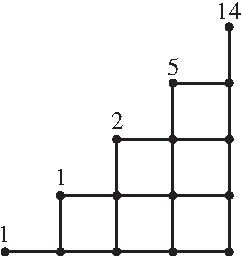
\includegraphics[width=0.33\linewidth]{images/CatalanPaths}
\caption{The lattice paths from \((0,0)\) to \((i,i)\) for \(i=0,1,2,3,4\).  The number of paths to the point \((i,i)\) is shown just above that point.\label{CatalanPaths}}
\end{figure}
~\par
\begin{enumerate}[label=(\alph*)]
 \item Explain why the number of lattice paths from \((0,0)\) to \((n,n)\) that go outside the triangle is the number of lattice paths from \((0,0)\) to \((n,n)\) that either touch or cross the line \(y=x+1\).%
\par\medskip\noindent%
\textbf{Solution.}\quad If a lattice path between \((0,0)\) and \((n,n)\) goes outside the triangle, it can only do so on an upstep. (A step from \((i,j)\) to \((i,j+1)\).) And an upstep must originate at a point with integer coordinates. If \(j\lt i\) an upstep from \((i,j))\) cannot leave the triangle. Thus to leave the triangle, the upstep must leave from a point of the form \((i,i)\), and go to \((i,i+1)\), which is on the line \(y=x+1\).%

~\par
\item Find a bijection between lattice paths from \((0,0)\) to \((n,n)\) that touch (or cross) the line \(y=x+1\) and lattice paths from \((-1,1)\) to \((n,n)\).%
\par\medskip\noindent%
\textbf{Solution.}\quad Suppose we have a lattice path form \((0,0)\) to \((n,n)\) which touches or crosses the line \(y=x+1\). Let \((k,k+1)\) be the first point on the line \(y=x+1\) that the lattice path touches. From that point, work backwards, replacing every upstep with a step one unit to the left and every rightstep with a step one unit down. The segment of the path you just changed will have moved left \(k+1\) times, so its leftmost \(x\) coordinate will be \(-1\), and it will have moved down \(k\) times, so its lowest \(y\) coordinate will be 1.  Thus we now have a lattice path from \((-1,1)\) to \((n,n)\). Further, given a lattice path from \((-1,1)\) to \((n,n)\), it must cross the line \(y=x+1\) at least once, because it starts above the line and ends below it. At the first point where such a path touches the line \(y=x+1\), say \((k',k'+1)\), work backwards replacing every upstep with a step to the left and every rightstep with a step downwards. The leftmost point on this path will have \(x\) coordinate 0, and the lowest point will have \(y\) coordinate 0, so the new path will be a lattice path from \((0,0)\) to \((n,n)\) that touches the line \(y=x+1\). Clearly these two processes reverse each other, and so they give us a bijection between paths form \((0,0)\) to \((n,n)\) that touch the line \(y=x+1\) and lattice lattice paths from \((-1,1)\) to \((n,n)\). Notice that geometrically what we are doing to get the bijection is to take the portion of a lattice path that goes from the initial point till the first touch of the line \(y=x+1\) and reflecting it around that line. This idea of reflection was introduced by Feller, and is called Feller's reflection principle.%

~\par
\item Find a formula for the number of lattice paths from \((0,0)\) to \((n,n)\) that do not cross the line \(y=x\).  The number of such paths is called a \emph{Catalan Number}\index{Catalan Number} and is usually denoted by \(C_n\).%
\par\medskip\noindent%
\textbf{Solution.}\quad \(C_n={2n\choose n} - {2n \choose n+1}={1\over n+1}{2n\choose n}.\)%

\end{enumerate}
\end{activity}
\begin{activity}[]\label{activity-6}
Your formula for the Catalan Number can be expressed as a binomial coefficient divided by an integer. Whenever we have a formula that calls for division by an integer, an ideal combinatorial explanation of the formula is one that uses the quotient principle. The purpose of this problem is to find such an explanation using diagonal lattice paths.\footnote{The result we will derive is called the Chung-Feller Theorem\index{Chung-Feller Theorem}; this approach is based of a paper of Wen-jin Woan ``Uniform Partitions of Lattice Paths and Chung-Feller Generalizations," \textsl{American Mathematics Monthly 58} June/July 2001, p556.\label{fn-1}} A diagonal lattice path that never goes below the \(y\)-coordinate of its first point is called a \terminology{Dyck Path}\index{Dyck path}. We will call a Dyck Path from \((0,0)\) to \((2n,0)\) a \terminology{Catalan Path}\index{Catalan Path} of length \(2n\). Thus the number of Catalan Paths of length \(2n\) is the Catalan Number \(C_n\).%
~\par
\begin{enumerate}[label=(\alph*)]
 \item If a Dyck Path has \(n\) steps (each an upstep or downstep), why do the first \(k\) steps form a Dyck Path for each nonnegative \(k\le n\)?%
\par\medskip\noindent%
\textbf{Solution.}\quad If no points on the path are lower than the first point, then no points among the first \(k\) steps are lower than the first point.%

~\par
\item Thought of as a curve in the plane, a diagonal lattice path can have many local maxima and minima, and can have several absolute maxima and minima, that is, several highest points and several lowest points. What is the \(y\)-coordinate of an absolute minimum point of a Dyck Path starting at \((0,0)\)?  Explain why a Dyck Path whose rightmost absolute minimum point is its last point is a Catalan Path.%
\par\medskip\noindent%
\textbf{Solution.}\quad Since the path starts at \((0,0)\) and can't go below it, the \(y\) coordinate of an absolute minimum must be zero. If the last point is an absolute minimum, then (because it ends with the same \(y\) coordinate with which it starts) the path has an even number \(2k\) of steps and ends at \((2k,0)\).%

~\par
\item Let \(D\) be the set of all diagonal lattice paths from \((0,0)\) to \((2n,0)\).  (Thus these paths can go below the \(x\)-axis.) Suppose we partition \(D\) by letting \(B_i\) be the set of lattice paths in \(D\) that have \(i\) upsteps (perhaps mixed with some downsteps) following the last absolute minimum.  How many blocks does this partition have?  Give a succinct description of the block \(B_0\).%
\par\medskip\noindent%
\textbf{Solution.}\quad The path must have \(n\) upsteps total, and so can have any number between 0 and \(n\) upsteps after the rightmost absolute minimum. Thus the partition has \(n+1\) blocks. Block \(B_0\) consists of the Catalan Paths.%

~\par
\item How many upsteps are in a Catalan Path?%
\par\medskip\noindent%
\textbf{Solution.}\quad \(n\).%

~\par
\item We are going to give a bijection between the set of Catalan Paths and the block \(B_i\) for each \(i\) between \(1\) and \(n\).  For now, suppose the value of \(i\), while unknown, is fixed.  We take a Catalan path and break it into three pieces.  The piece \(F\) (for ``front'') consists of all steps before the \(i\)th upstep in the Catalan path.  The piece \(U\) (for ``up'') consists of the \(i\)th upstep.  The piece \(B\) (for ``back'') is the portion of the path that follows the \(i\)th upstep.  Thus we can think of the path as \(FUB\).  Show that the function that takes \(FUB\) to \(BUF\) is a bijection from the set of Catalan Paths onto the block \(B_i\) of the partition.  (Notice that \(BUF\) can go below the \(x\) axis.)%
\par\medskip\noindent%
\textbf{Solution.}\quad Since we are starting with a Catalan path, the point on the path at the beginning of the \(i\)th upstep must have \(y\) coordinate greater or equal to than zero. Thus wherever we start the sequence \(F\) of upsteps and downsteps, a path constructed by this sequence never goes lower than its starting point. Thus in \(BUF\) the last absolute minimum is either right before the \(U\) or earlier. But \(B\) is the final segment of a Catalan Path, so its final point is at least as low as its starting point. Thus the point at the beginning of the \(U\) in \(BUF\) is an absolute minimum, and there are \(i\) upsteps after that local minimum. If we take two different sequences and rearrange them in the same way, we get two different sequences, so the function we just described is a one-to-one function. If we take an arbitrary diagonal lattice path from \((0,0)\) to \((2n,0)\), let \(U'\) be the first upstep after the last absolute minimum, \(F'\) be the portion of the path that follows \(U'\), and \(B'\) be the portion that precedes \(U'\), then \(F'U'B'\) is a Catalan Path, and \(U'\) is its \(i\)th upstep if and only if in \(B'U'F'\) there are \(i\) upsteps after the last absolute minimum. Thus the mapping from \(FUB\) to \(BUF\) is a bijection.%

~\par
\item Explain how you have just given another proof of the formula for the Catalan Numbers.%
\par\medskip\noindent%
\textbf{Solution.}\quad We have taken the set of all \(2n\choose n\) diagonal lattice paths of length \(2n\) from \((0,0)\) to \((2n,0)\) and partitioned it into \(n+1\) blocks all of size \(C_n\). Thus by the quotient principle, \(C_n={1\over
n+1}{2n
\choose n}\).%

\end{enumerate}
\end{activity}
\typeout{************************************************}
\typeout{Subsection  The Binomial Theorem}
\typeout{************************************************}
\subsection[{The Binomial Theorem}]{The Binomial Theorem}\label{subsection-2}
\begin{activity}[]\label{Conjecturebinomthm}
We know that \((x+y)^2 = x^2+2xy+y^2\). Multiply both sides by \((x+y)\) to get a formula for \((x+y)^3\) and repeat to get a formula for \((x+y)^4\). Do you see a pattern? If so, what is it? If not, repeat the process to get a formula for \((x+y)^5\) and look back at {$\langle\langle$Unresolved xref, reference "Pascaltriangle"; check spelling or use "provisional" attribute$\rangle\rangle$} to see the pattern. Conjecture a formula for \((x+y)^n\).%
\par\medskip\noindent%
\textbf{Solution.}\quad \((x+y)^3=x^3+2x^2y +xy^2+x^2y+ +2xy^2 +y^3=x^3+3x^2y++3xy^2+y^3\).%
\par
Similarly, \((x+4)^4=x^4+4x^3y+6x^2y^2+4xy^3+y^4\),%
\par
and \((x+y)^5=x^5+5x^4y+10x^3y^2+10x^2y^3+5xy^4+y^5.\) The pattern is that the coefficient of \(x^iy^j\) is \(i+j\choose i\) which is the same as \(i+j\choose j\). Said differently, the coefficient of \(x^{n-i}y^i\) is \(n\choose i\) or the coefficient of \(x^iy^{n-i}\) is \(n\choose
i\). We conjecture that%
\begin{equation*}
(x+y)^n=\sum_{i=0}^n {n\choose i}x^{n-i}y^i.
\end{equation*}
%
\par
(The reason for putting \(x^{n-i}y^i\) into the sum is so that as \(i\) goes from 0 to \(n\), the powers of \(x\) decrease from \(n\) to 0.)%
\end{activity}
\begin{activity}[]\label{activity-8}
When we apply the distributive law \(n\) times to \((x+y)^n\), we get a sum of terms of the form \(x^iy^{n-i}\) for various values of the integer \(i\).%
~\par
\begin{enumerate}[label=(\alph*)]
 \item If it is clear to you that each term of the form \(x^iy^{n-i}\) that we get comes from choosing an \(x\) from \(i\) of the \((x+y)\) factors and a \(y\) from the remaining \(n-i\) of the factors and multiplying these choices together, then answer this part of the problem and skip the next part.  Otherwise, do the next part instead of this one.  In how many ways can we choose an \(x\) from \(i\) terms and a \(y\) from \(n-i\) terms?%
\par\medskip\noindent%
\textbf{Solution.}\quad The number of ways to choose an \(x\) from \(i\) of the factors and a \(y\) from the remaining ones is the way to choose the \(i\) factors from the \(n\) factors; that is, \(n\choose i\).%

~\par
\item Expand the product \((x_1 +y_1)(x_2 +y_2)(x_3+y_3)\).%
\par\medskip\noindent%
\textbf{Solution.}\quad %
\begin{align*}
(x_1+y_1)(x_2+y_2)(x_3+y_3)=x_1x_2x_3 \!\!\amp +\amp \!\!x_1x_2y_3+x_1y_2x_3+\\
y_1x_2x_3+x_1y_2y_3+y_1x_2y_3 \!\!\amp +\amp \!\! y_1y_2x_3+y_1y_2y_3.
\end{align*}
%

~\par
\item What do you get when you substitute \(x\) for each \(x_i\) and \(y\) for each \(y_i\)?%
\par\medskip\noindent%
\textbf{Solution.}\quad When you substitute \(x\) for each \(x_i\) and \(y\) for each \(y_i\), you get \((x+y)^3=x^3+3x^2y+3xy^2+y^3\).%

~\par
\item Now imagine expanding%
\begin{equation*}
(x_1+y_1)(x_2+y_2)\cdots (x_n+y_n).
\end{equation*}
Once you apply the commutative law to the individual terms you get, you will have a sum of terms of the form%
\begin{equation*}
x_{k_1}x_{k_2}\cdots x_{k_i}\cdot y_{j_1}y_{j_2}\cdots
y_{j_{n-i}}.
\end{equation*}
What is the set \(\{k_1,k_2,\ldots, k_i\}\cup \{j_1,j_2,\ldots, j_{n-i}\}\)?%
\par\medskip\noindent%
\textbf{Solution.}\quad \(\{k_1,k_2,\ldots, k_i\}\cup
\{j_1,j_2,\ldots, j_{n-i}\}=\{1,2,\ldots, n\}\).%

~\par
\item In how many ways can you choose the set \(\{k_1,k_2,\ldots, k_i\}\)?%
\par\medskip\noindent%
\textbf{Solution.}\quad You can choose the set \(\{k_1,k_2,\ldots k_i\}\) in \(n\choose i\) ways.%

~\par
\item Once you have chosen this set, how many choices do you have for \(\{j_1,j_2,\ldots, j_{n-i}\}\)?%
\par\medskip\noindent%
\textbf{Solution.}\quad Once you have chosen the set of \(k\)s, there is just one way to choose the set of \(j\)s.%

~\par
\item If you substitute \(x\) for each \(x_i\) and \(y\) for each \(y_i\), how many terms of the form \(x^iy^{n-i}\) will you have in the expanded product%
\begin{equation*}
(x_1+y_1)(x_2+y_2)\cdots (x_n+y_n)=(x+y)^n?
\end{equation*}
%
\par\medskip\noindent%
\textbf{Solution.}\quad If you substitute \(x\) for \(x_i\) and substitute \(y\) for \(y_i\), you will get \(n\choose i\) terms of the form \(x^iy^{n-i}\).%

~\par
\item How many terms of the form \(x^{n-i}y^i\) will you have?%
\par\medskip\noindent%
\textbf{Solution.}\quad You will also get \(n\choose i\) terms of the form \(x^{n-i}y^i\).%

~\par
\item Explain how you have just proved your conjecture from \hyperref[Conjecturebinomthm]{Problem~\ref{Conjecturebinomthm}}.  The theorem you have proved is called the \emph{Binomial Theorem}.\index{Binomial Theorem}%
\par\medskip\noindent%
\textbf{Solution.}\quad We have proved that the coefficient of \(x^iy^{n-i}\) in \((x+y)^n\) is \(n\choose i\), or equivalently that the coefficient of \(x^{n-i}y^i\) in \((x+y)^n\) is \(n\choose i\).%

\end{enumerate}
\end{activity}
\begin{activity}[]\label{activity-9}
What is \(\sum_{i=1}^n {10\choose i}3^i\)?%
\par\medskip\noindent%
\textbf{Solution.}\quad \(\sum_{i=1}^n {10\choose i}3^i=\sum_{i=0}^n
{10\choose i}3^i-{10\choose 0}3^0 =(1+3)^{10}-1=4^{10}-1\)%
\end{activity}
\begin{activity}[]\label{activity-10}
What is \({n\choose 0}-{n\choose 1}+{n\choose 2}-\cdots \pm
{n\choose n}\) if \(n\) is an integer bigger than 0?%
\par\medskip\noindent%
\textbf{Solution.}\quad The sum is \(0\) because it is \((-1+1)^n\).%
\end{activity}
\begin{activity}[]\label{activity-11}
Explain why%
\begin{equation*}
\sum_{i=0}^m{m\choose i}{n\choose k-i} = {m+n\choose
k}.
\end{equation*}
Find two different explanations.%
\par\medskip\noindent%
\textbf{Solution.}\quad When we expand both sides of \((x+y)^m(x+y)^n=(x+y)^{m+n}\) by the binomial theorem we get \(\sum_{i=0}^m{m\choose i}{n\choose  k-i}\) as the coefficient of \(x^{m+n-k}y^k\) on the left hand side and \(m+n\choose k\) on the right hand side.%
\par
For a second explanation, to choose \(k\) elements out of the union of an \(m\)-element set and a disjoint \(n\)-element set, chose some number \(i\le m\) of them from the \(m\)-element set and the remaining \(k-i\) of them from the \(n\)-element set. The sum on the left hand side of the equation simply sums the number of such choices over all possible \(i\), and the binomial coefficient on the right hand side of the equation says we will end up choosing \(k\) elements from among our \(m+n\) elements.%
\end{activity}
\begin{activity}[]\label{activity-12}
From the symmetry of the binomial coefficients, it is not too hard to see that when \(n\) is an odd number, the number of subsets of \(\{1,2,\ldots,n\}\) of odd size equals the number of subsets of \(\{1,2,\ldots,n\}\) of even size. Is it true that when \(n\) is even the number of subsets of \(\{1,2,\ldots,n\}\) of even size equals the number of subsets of odd size? Why or why not?%
\par\medskip\noindent%
\textbf{Solution.}\quad It is true, because if \(n>0\), when you expand \((1-1)^n\) by the binomial theorem, you get an alternating sum of binomial coefficients equal to 0, and so the sum of the binomial coefficients \(n\choose i\) with \(i\) even must equal the sum of the binomial coefficients \(n\choose i\) with \(i\) odd.%
\end{activity}
\begin{activity}[]\label{activity-13}
What is \(\sum_{i=0}^n i{n\choose i}\)? (Hint: think about how you might use calculus.)%
\par\medskip\noindent%
\textbf{Solution.}\quad \(\sum_{i=0}^n({n\choose i}x^i = (1+x)^n\). Taking derivatives of both sides gives us \(\sum_{i=0}^ni{n\choose i}x^{i-1} = n(1+x)^{n-1}.\). Now substitute 1 for \(x\) and you get \(\sum_{i=0}^n i{n\choose i} = n2^{n-1}\).%
\end{activity}
Notice how the proof you gave of the binomial theorem was a counting argument. It is interesting that an apparently algebraic theorem that tells us how to expand a power of a binomial is proved by an argument that amounts to counting the individual terms of the expansion. Part of the reason that combinatorial mathematics turns out to be so useful is that counting arguments often underlie important results of algebra. As the algebra becomes more sophisticated, so do the families of objects we have to count, but nonetheless we can develop a great deal of algebra on the basis of counting.%
\typeout{************************************************}
\typeout{Subsection  The pigeonhole principle}
\typeout{************************************************}
\subsection[{The pigeonhole principle}]{The pigeonhole principle}\label{subsection-3}
\begin{activity}[]\label{elevencoins}
American coins are all marked with the year in which they were made. How many coins do you need to have in your hand to guarantee that on two (at least) of them, the date has the same last digit? (When we say ``to guarantee that on two (at least) of them,\dots{}'' we mean that you can find two with the same last digit. You might be able to find three with that last digit, or you might be able to find one pair with the last digit 1 and one pair with the last digit 9, or any combination of equal last digits, as long as there is at least one pair with the same last digit.)%
\par\medskip\noindent%
\textbf{Solution.}\quad Since there are ten possible last digits, you need at least 11 coins, and with 11 coins, at least two last digits must be the same.%
\end{activity}
There are many ways in which you might explain your answer to \hyperref[elevencoins]{Activity~\ref{elevencoins}}. For example, you can partition the coins according to the last digit of their date; that is, you put all the coins with a given last digit in a block together, and put no other coins in that block; repeating until all coins are in some block. Then you have a partition of your set of coins. If no two coins have the same last digit, then each block has exactly one coin. Since there are only ten digits, there are at most ten blocks and so by the sum principle there are at most ten coins. In fact with ten coins it is possible to have no two with the same last digit, but with 11 coins some block must have at least two coins in order for the sum of the sizes of at most ten blocks to be 11. This is one explanation of why we need 11 coins in \hyperref[elevencoins]{Activity~\ref{elevencoins}}. This kind of situation arises often in combinatorial situations, and so rather than always using the sum principle to explain our reasoning , we enunciate another principle which we can think of as yet another variant of the sum principle. The \terminology{pigeonhole principle}\index{pigeonhole principle} states that%
\begin{quote}If we partition a set with more than \(n\) elements into \(n\) parts, then at least one part has more than one element.%
\end{quote}
The pigeonhole principle gets its name from the idea of a grid of little boxes that might be used, for example, to sort mail, or as mailboxes for a group of people in an office. The boxes in such grids are sometimes called pigeonholes in analogy with stacks of boxes used to house homing pigeons when homing pigeons were used to carry messages. People will sometimes state the principle in a more colorful way as ``if we put more than \(n\) pigeons into \(n\) pigeonholes, then some pigeonhole has more than one pigeon.''%
\begin{activity}[]\label{activity-15}
Show that if we have a function from a set of size \(n\) to a set of size less than \(n\), then \(f\) is not one-to-one.%
\par\medskip\noindent%
\textbf{Solution.}\quad Let \(T\) be the set of size less than \(n\), and \(S\) be the set of size \(n\). Let \(B_j=\{i|f(i)=j\}\) for each \(j\) in \(T\). Then the nonempty sets among the \(B_j\)s form a partition of \(S\) and the number of blocks is less than the size of \(S\). Therefore by the pigeonhole principle, there is at least one block with at least two elements, so there are two elements \(i_1\) and \(i_2\) such that \(f(i_1)=f(i_2)\).%
\end{activity}
\begin{activity}[]\label{activity-16}
Show that if \(S\) and \(T\) are finite sets of the same size, then a function \(f\) from \(S\) to \(T\) is one-to-one if and only if it is onto.%
\par\medskip\noindent%
\textbf{Solution.}\quad First suppose that \(f\) is a one-to-one function from \(S\) to \(T\), sets which have the same size. Let \(B_j=\{i|f(i)=j\}\) for each \(j\) in \(T\)..  If \(f\) is not onto, then the number of nonempty sets \(B_j\) is smaller than the number of elements of \(T\) and thus is smaller than the size of \(S\). The nonempty sets \(B_j\) are a partition of \(S\). But then by the pigeonhole principle, some nonempty \(B_j\) has two or more elements, contradicting the assumption that \(f\) is one-to-one. Therefore if \(f\) is one-to-one, then it is onto. Now suppose that \(f\) is an onto function from \(S\) to \(T\), sets of the same size. Again let \(B_j =\{i|f(i)=j\}\) for each \(j\) in \(T\). The size of the union of the sets \(B_j\) is, by the sum principle, the sum of their sizes. Since \(f\) is onto, each \(B_j\) has at least one element. Since the number of sets \(B_j\) is the number of elements of \(S\), if one of those sets has more than one element, the the size of their union is more than the size of \(S\), which is a contradiction since they are subsets of \(S\). Therefore each set \(B_j\) has exactly one element and therefore \(f\) is one-to-one.%
\end{activity}
\begin{activity}[]\label{activity-17}
~\par
\begin{enumerate}[label=(\alph*)]
 \item There is a \terminology{generalized pigeonhole principle}\index{pigeonhole principle!generalized} which says that if we partition a set with more than \(kn\) elements into \(n\) blocks, then at least one block has at least \(k+1\) elements. Prove the generalized pigeonhole principle.%
\par\medskip\noindent%
\textbf{Solution.}\quad Suppose we partition a set \(S\) of more than \(kn\) elements into \(n\) blocks. If each block has at most \(k\) elements, the by the sum principle the size of \(S\) is at most \(kn\). But this is a contradiction, so some block has at least \(k+1\) elements.%

~\par
\item All the powers of five end in a five, and all the powers of two are even. Show that for for some integer \(n\), if you take the first \(n\) powers of a prime other than two or five, one must have ``01'' as the last two digits.%
\par\medskip\noindent%
\textbf{Solution.}\quad If we take 40 powers of such a prime, either one will end in ``01'' or some two, say \(p^i\) and \(p^j\) with \(i>j\) must have the same last two digits by the pigeon hole principle. Then \(p^i-p^j=100k\) for some integer \(k\). Thus \(p^j(p^{i-j} -1)\) must be a multiple of 100, and since neither 2 nor 5 divide \(p\), \(p^{i-j} -1 = 100k'\) for some integer \(k'\) then \(p^{i-j} = 100k'+1\), so the last two digits of \(p^{i-j}\) must be ``01.''%

\end{enumerate}
\end{activity}
\begin{activity}[]\label{R_3_3_}
Show that in a set of six people, there is a set of at least three people who all know each other, or a set of at least three people none of whom know each other. (We assume that if person 1 knows person 2, then person 2 knows person 1.)%
\par\medskip\noindent%
\textbf{Solution.}\quad By the generalized pigeonhole principle, person 1 either knows at least three people or doesn't know at least three people. Suppose person 1 knows three people. Then either two of these people know each other, giving us, with person 1, three mutual acquaintances, or no two of these people know each other, giving us three mutual strangers. On the other hand if there are three people person 1 does not know, then either two of these people don't know each other, giving us, with person 1, three mutual strangers, or all three of these people know each other, giving us three mutual acquaintances.%
\end{activity}
\begin{activity}[]\label{notR_3_3_}
Draw five circles labeled Al, Sue, Don, Pam, and Jo. Find a way to draw red and green lines between people so that every pair of people is joined by a line and there is neither a triangle consisting entirely of red lines or a triangle consisting of green lines. What does \hyperref[R_3_3_]{Problem~\ref{R_3_3_}} tell you about the possibility of doing this with six people's names? What does this problem say about the conclusion of \hyperref[R_3_3_]{Problem~\ref{R_3_3_}} holding when there are five people in our set rather than six?%
\par\medskip\noindent%
\textbf{Solution.}\quad In the figure that follows, we use solid lines for red and dashed lines for green. Clearly there is no solid triangle and no dashed triangle.%
\begin{figure}
\centering
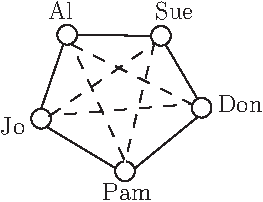
\includegraphics[width=0.33\linewidth]{images/NonRamsey5}
\end{figure}
\hyperref[R_3_3_]{Activity~\ref{R_3_3_}} says you can't do this with six people's names. This problem says that the conclusion of \hyperref[R_3_3_]{Activity~\ref{R_3_3_}} does not hold when you have five people.%
\end{activity}
\typeout{************************************************}
\typeout{Subsection  Ramsey Numbers}
\typeout{************************************************}
\subsection[{Ramsey Numbers}]{Ramsey Numbers}\label{Ramseysection}
Activity~\hyperref[R_3_3_]{\ref{R_3_3_}}--\hyperref[notR_3_3_]{\ref{notR_3_3_}} together show that six is the smallest number \(R\) with the property that if we have \(R\) people in a room, then there is either a set of (at least) three mutual acquaintances or a set of (at least) three mutual strangers. Another way to say the same thing is to say that six is the smallest number so that no matter how we connect 6 points in the plane (no three on a line) with red and green lines, we can find either a red triangle or a green triangle. There is a name for this property. The \terminology{Ramsey Number} \(R(m,n)\) is the smallest number \(R\) so that if we have \(R\) people in a room, then there is a set of at least \(m\) mutual acquaintances or at least \(n\) mutual strangers. There is also a geometric description of Ramsey Numbers; it uses the idea of a \emph{complete graph} on \(R\) vertices. A \emph{complete graph}\index{graph!complete} on \(R\) vertices consists of \(R\) points in the plane together with line segments (or curves) connecting each two of the \(R\) vertices.\footnote{As you may have guessed, a complete graph is a special case of something called a graph.  The word graph will be defined in \hyperref[graphsection]{Subsection~}.\label{fn-2}} The points are called \terminology{vertices}\index{vertex!of a complete graph}\index{vertex} and the line segments are called \terminology{edges}\index{edge!of a complete graph}\index{edge}. In \hyperref[completegraph]{Figure~\ref{completegraph}} we show three different ways to draw a complete graph on four vertices. We use \(K_n\) to stand for a complete graph on \(n\) vertices.%
\begin{figure}
\centering
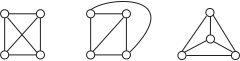
\includegraphics[width=0.33\linewidth]{images/threeK4s}
\caption{Three ways to draw a complete graph on four vertices\label{completegraph}}
\end{figure}
Our geometric description of \(R(3,3)\) may be translated into the language of graph theory (which is the subject that includes complete graphs) by saying \(R(3,3)\) is the smallest number \(R\) so that if we color the edges of a \(K_R\) with two colors, then we can find in our picture a \(K_3\) all of whose edges have the same color.  The graph theory description of \(R(m,n)\) is that \(R(m,n)\) is the smallest number \(R\) so that if we color the edges of a \(K_R\) with red and green, then we can find in our picture either a \(K_m\) all of whose edges are red or a \(K_n\) all of whose edges are green. Because we could have said our colors in the opposite order, we may conclude that \(R(m,n) = R(n,m)\). In particular \(R(n,n)\) is the smallest number \(R\) such that if we color the edges of a \(K_R\) with two colors, then our picture contains a \(K_n\) all of whose edges have the same color.%
\begin{activity}[]\label{activity-20}
Since \(R(3,3)=6\), an uneducated guess might be that \(R(4,4)=8\). Show that this is not the case.%
\par\medskip\noindent%
\textbf{Solution.}\quad In the graph of \hyperref[NonRamsey8]{Figure~\ref{NonRamsey8}}, each vertex has three dashed lines emanating from it, and there are no dashed lines connecting any of the three vertices adjacent to it by dashed lines. Each vertex has four solid lines emanating from it, and no three of the four vertices adjacent to it by solid lines are all adjacent by solid lines. Thus there is no solid line \(K_4\) and there is no dashed line \(K_4\).%
\begin{figure}
\centering
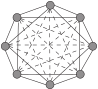
\includegraphics[width=0.33\linewidth]{images/NonRamsey8}
\caption{A graph showing \(R(4,4) \gt 8\)\label{NonRamsey8}}
\end{figure}
\end{activity}
\begin{activity}[]\label{activity-21}
Show that among ten people, there are either four mutual acquaintances or three mutual strangers. What does this say about \(R(4,3)\)?%
\par\medskip\noindent%
\textbf{Solution.}\quad Take a person, say person 1. If person has six acquaintances, then by \hyperref[R_3_3_]{Activity~\ref{R_3_3_}} among them there are either three mutual strangers, in which case we are done, or three mutual acquaintances. These three acquaintances together with person 1 form a set of 4 mutual acquaintances in which case we are again done. Thus we may assume Person 1 has at most 5 acquaintances, and so has four non-acquaintances. Now either all four of these people are acquainted, in which case we are done, or else two of them are not acquainted. Then these two people, together with person 1 make three mutual nonacquaintances. Therefore in every possible case, we have either four mutual acquaintances or three mutual strangers. This means that \(R(4,3) \le 10\).%
\end{activity}
\begin{activity}[]\label{OddNoPeople}
Show that among an odd number of people there is at least one person who is an acquaintance of an even number of people and therefore also a stranger to an even number of people.%
\par\medskip\noindent%
\textbf{Solution.}\quad Suppose we add, for each person, the number of people with whom he or she is acquainted. Then we get twice the number of acquaintance edges in the graph of acquaintance and non-acquaintance relationships. Thus the sum must be even. But if each person among an odd number of people were acquainted with an odd number of people, then the sum would be odd. Since this is a contradiction, among an odd number of people, there must be at least one who is acquainted with an even number of people. Since the number of people different from this person is even, the number of people with whom this person is not acquainted is also even.%
\end{activity}
\begin{activity}[]\label{R_4_3_not8}
Find a way to color the edges of a \(K_8\) with red and green so that there is no red \(K_4\) and no green \(K_3\).%
\par\medskip\noindent%
\textbf{Solution.}\quad In the graph shown in \hyperref[NonRamsey8]{Figure~\ref{NonRamsey8}}, there is no \(K_3\) whose edges are dashed, and no \(K_4\) whose edges are solid. By symmetry, to verify this you need only look at vertex 1 and vertices connected to it by either dashed lines or by solid lines.%
\end{activity}
\begin{activity}[]\label{activity-24}
Find \(R(4,3)\).%
\par\medskip\noindent%
\textbf{Solution.}\quad \(R(4,3)=9\). In \hyperref[R_4_3_not8]{Activity~\ref{R_4_3_not8}} we showed that \(R(4,3)\) is more than 8. So we must show that if we have nine people, we either have 4 mutual acquaintances or three mutual strangers. By \hyperref[OddNoPeople]{Activity~\ref{OddNoPeople}} there is at least one person (say person A) who is acquainted with an even number of people. If person A is acquainted with six or more people, then among these six people, there are either three mutual acquaintances or three mutual strangers. If there are three mutual strangers, we are done; if there are three mutual acquaintances, they, together with Person A are four mutual acquaintances. Thus we may assume Person A is acquainted with at most four people. Thus person A is a stranger to at least four people. If two of these people are strangers, then they, together with person A form three mutual strangers and we are done. Otherwise all of these people know each other and we have at least four mutual acquaintances, and so in every possible situation, we have either four mutual acquaintances or three mutual strangers.%
\end{activity}
As of this writing, relatively few Ramsey Numbers are known. \(R(3,n)\) is known for \(n\lt 10\), \(R(4,4) = 18\), and \(R(5,4)=R(4,5)=25\).%
\typeout{************************************************}
\typeout{Section 0.3 Supplementary Chapter Problems}
\typeout{************************************************}
\section[{Supplementary Chapter Problems}]{Supplementary Chapter Problems}\label{section-3}
\leavevmode%
\begin{enumerate}
\item\hypertarget{compositiondefinition}{}(interesting) Remember that we can write \(n\) as a sum of \(n\) ones.  How many plus signs do we use?  In how many ways may we write \(n\) as a sum of a list of \(k\) positive numbers?  Such a list is called a \emph{composition}\index{composition} of \(n\) into \(k\) parts.\index{composition!\(k\) parts}\index{composition!\(k\) parts!number of} We use \(n-1\) plus signs. Write down such a sum and choose \(k-1\) of the plus signs. Then each string of ones and plusses between two chosen plus signs, before the first chosen plus sign or after the last chosen one corresponds to a part of a composition of \(n\). Thus the number of compositions of \(n\) with \(k\) parts is the number of ways to choose the \(k-1\) places, which is \(n-1\choose k-1\).%
%
\item\hypertarget{composition_numberof}{}In \hyperlink{compositiondefinition}{Problem~1} we defined a composition of \(n\) into \(k\) parts.  What is the total number of compositions of \(n\) (into any number of parts). \index{compositions!number of} The total number of compositions is the number of ways to choose a subset of the plus signs which is \(2^{n-1}\).%
%
\item\hypertarget{GreyCode}{}(essential for this or the next section) Write down a list of all 16 0-1 sequences of length four starting with 0000 in such a way that each entry differs from the precious one by changing just one digit.  This is called a Grey Code.\index{Grey Code}  That is, a \emph{Grey Code} for 0-1 sequences of length \(n\) is a list of the sequences so that each entry differs from the previous one in exactly one place.  Can you describe how to get a Grey Code for 0-1 sequences of length five from the one you found for sequences of length 4?  Can you describe how to prove that there is a Grey code for sequences of length \(n\)? (One of many) 0000, 0001, 0011, 0010, 0110, 0111, 0101, 0100, 1100, 1101, 1111, 1110, 1010, 1011, 1001, 1000. To get a code for sequences of length 5, put a zero at the end of each of the sequences we have. Follow that revised sequence by 10001, and write the remainder of the sequence in reverse order with a 1 at the end of each term. (Don't reverse the individual length four sequences, just the sequence of sequences!) We just, in essence, described the inductive step of an inductive proof that Grey Codes exist for sequences of any length.%
%
\item\hypertarget{li-4}{}(interesting) Use the idea of a Grey Code from \hyperlink{GreyCode}{Problem~3} to prove bijectively that the number of even-sized subsets of an \(n\)-element set equals the number of odd-sized subsets of an \(n\)-element set. Each sequence in the Grey Code is the characteristic function of a set, and the number of elements of the set is the number of ones in the sequence. Since each sequence differs in just one place from the preceding one, the sequences alternate between having an even number of ones and an odd number of ones. Since the first sequence is all zeros and there are \(2^n\) sequences, the last one has an odd number of zeros. Thus the map that takes each sequence except the last to the next one, and takes the last to the first is a bijection between the characteristic functions of sets with an even number of elements and sets with an odd number of elements.%
%
\item\hypertarget{li-5}{}(interesting) A list of parentheses is said to be balanced if there are the same number of left parentheses as right, and as we count from left to right we always find at least as many left parentheses as right parentheses.  For example, (((()()))()) is balanced and ((()) and (()()))(() are not.  How many balanced lists of \(n\) left and \(n\)  right parentheses are there? The number is the Catalan number: we get a bijection between balanced lists of parentheses and Catalan paths by sending each left paren to an upstep and each right paren to a downstep. The condition that there are always as many left parentheses as right ensures we never go below the \(x\) axis.%
%
\item\hypertarget{li-6}{}(difficult) Suppose we plan to put six distinct computers in a network as shown in \hyperref[hexagonalnetwork]{Figure~\ref{hexagonalnetwork}}.  The lines show which computers can communicate directly with which others.  Consider two ways of assigning computers to the nodes of the network different if there are two computers that communicate directly in one assignment and that don't communicate directly in the other.  In how many different ways can we assign computers to the network? \begin{figure}
\centering
\includegraphics[width=0.73\linewidth]{images/}
\caption{A computer network.\label{hexagonalnetwork}}
\end{figure}
 We consider two assignments of computers to be equivalent if in both assignments, each computer communicates directly with exactly the same computers. This partitions the set of all \(6!\) computer assignments into blocks of \(48\) computers each. Thus we have \(720/48=15\) ways to assign the computers to the network.%
%
\item\hypertarget{li-7}{}(interesting) In a circular ice cream dish we are going to put four distinct scoops of ice cream chosen from among twelve flavors.  Assuming we place four scoops of the same size as if they were at the corners of a square, and recognizing that moving the dish doesn't change the way in which we have put the ice cream into the dish, in how many ways may we choose the ice cream and put it into the dish? Each ice cream arrangement is equivalent to three others, the ones we get by rotating the dish. This divides the arrangements of four flavors of ice cream into blocks of size 4. Thus we may arrange the ice cream we have chosen in the dish in \(4!/4=6\) ways. We may choose the ice cream in \({12\choose 4}=495\) ways, and so we may choose it and put it into the dish in 2970 ways.%
%
\item\hypertarget{li-8}{}(interesting) In as many ways as you can, show that \({n\choose k}{n-k\choose m} =
{n\choose m}{n-m\choose k}\). You can prove this by plugging in the formula for \(n\choose k\) on both sides and cancelling stuff until you get the same thing on both sides. However a much more interesting proof is that the right hand side counts the number of ways to choose a \(k\)-element set form an \(n\)-element set and then choose an \(m\)-element set from what remains. The left hand side counts the number of ways to first chose a \(k\)-element subset from the \(n\)-element set and then choose an \(m\)-element subset from what remains. Thus in both cases you are counting the number of ways to choose an ordered pair consisting of an \(m\)-element subset and a disjoint \(k\)-element subset from an \(n\)-element set. You can also base a proof on the observation that \((x+y+x)^n=
\sum_{k=0}^n{n\choose k}(x+y)^kz^{n-k}\) and \((x+y+z)^n=\sum_{m=0}^n{n\choose m}x^m(y+z)^{n-m}\) and asking for the coefficient of \(x^my^{n-m-k}z^k\). You do have to use the binomial theorem with an eye to the result you are looking for, however.%
%
\item\hypertarget{li-9}{}(interesting) A tennis club has \(4n\) members.  To specify a doubles match, we choose two teams of two people.  In how many ways may we arrange the members into doubles matches so that each player is in one doubles match?  In how many ways may we do it if we specify in addition who serves first on each team? We now have many methods for solving this problem. Perhaps the easiest is to list all \((4n)\) people and take them in groups of four for doubles matches, with the first two in a group of four as one team and the second two as another team. We note that interchanging the \(n\) blocks of 4 does not change the matches, nor does interchanging the two people on a team nor interchanging the two teams. Thus we have \((4n)!/n!2^{3n}\) ways to arrange the matches. If we are to say who serves first on each team, we might as well say it is the first of the two listed, so now we have \((4n)!/n!2^n\) ways to arrange the matches.%
%
\item\hypertarget{li-10}{}A town has \(n\) streetlights running along the north side of main street.  The poles on which they are mounted need to be painted so that they do not rust.  In how many ways may they be painted with red, white, blue, and green if an even number of them are to be painted green? We can think of first choosing the set of even size of poles to be painted green, and the painting the remaining poles red, white, and blue. We may do this in \(\sum_{k=0}^{\lfloor n/2\rfloor}{n\choose 2k}3^{n-2k}\) ways.%
%
\item\hypertarget{pingpongpaint}{}We have \(n\) identical ping-pong balls.  In how many ways may we paint them red, white, blue, and green? We can line up the identical ping-pong balls and break them into four groups, those of each color, by inserting dividers. If we want to paint at least one in each color, we can choose three of the spaces between the balls in which to insert dividers, so we can paint them in \(n-1\choose k\). But the problem didn't require us to use each color, so we can put two dividers adjacent to each other. Thus there are \(n+1\) places where we can put the first divider (putting it before all the balls means we use no red, and putting it after all of them means we use no green. Now there are \(n+2\) places where we can put the second divider, including before or after the first, and \(n+3\) places where we can put the third divider. However if we interchange two dividers we still paint the balls before the first divider red, those between then next two white, and so on. Thus \(3!=6\) of these arrangements of balls and dividers correspond to the same paint job, so the number of ways to paint the balls is \({(n+1)(n+2)(n+3)\over6} ={n+3\choose
3}\). This suggests that another way to think of the problem is to consider \(n+3\) slots in a row, and fill \(n\) of them with balls and \(3\) of them with dividers; since the balls are identical and the dividers might as well be identical, the number of ways to do this is the number of ways to choose the slots that get dividers.%
%
\item\hypertarget{li-12}{}We have \(n\) identical ping-pong balls.  In how many ways may we paint them red, white, blue, and green if we use green paint on an even number of them? We first decide how many balls to paint green, then paint the remainder with the other three colors as in \hyperlink{pingpongpaint}{Problem~11} This gives us%
\begin{equation*}
\sum_{k=0}^{\lfloor n/2\rfloor}{n-2k+2\choose 2}
\end{equation*}
ways to paint the balls.%
%
\end{enumerate}
\typeout{************************************************}
\typeout{Chapter 1 Applications of Induction and Recursion in Combinatorics and Graph Theory}
\typeout{************************************************}
\chapter[{Applications of Induction and Recursion in Combinatorics and Graph Theory}]{Applications of Induction and Recursion in Combinatorics and Graph Theory}\label{InductionRecursion}
\typeout{************************************************}
\typeout{Section 1.1 Some Examples of Mathematical Induction}
\typeout{************************************************}
\section[{Some Examples of Mathematical Induction}]{Some Examples of Mathematical Induction}\label{sec_induction-examples}
\typeout{************************************************}
\typeout{Introduction  }
\typeout{************************************************}
In Chapter 1 ({$\langle\langle$Unresolved xref, reference "SubsetsByInduction"; check spelling or use "provisional" attribute$\rangle\rangle$}), we used the principle of mathematical induction to prove that a set of size \(n\) has \(2^n\) subsets. If you were unable to do that problem and you haven't yet read {$\langle\langle$Unresolved xref, reference "Induction"; check spelling or use "provisional" attribute$\rangle\rangle$} (a portion of which is repeated here), you should do so now.%
\typeout{************************************************}
\typeout{Subsection  Mathematical induction}
\typeout{************************************************}
\subsection[{Mathematical induction}]{Mathematical induction}\label{subsection-5}
\typeout{************************************************}
\typeout{Introduction  }
\typeout{************************************************}
The \emph{principle of mathematical induction}\index{mathematical induction!principle of}\index{principle of mathematical induction}\index{induction!mathematical, the principle of} states that%
\begin{quote}In order to prove a statement about an integer \(n\), if we can \leavevmode%
\begin{enumerate}
\item\hypertarget{li-13}{}Prove the statement when \(n=b\), for some fixed integer \(b\)%
\item\hypertarget{li-14}{}Show that the truth of the statement for \(n=k-1\) implies the truth of the statement for \(n=k\) whenever \(k>b\),%
\end{enumerate}
 then we can conclude the statement is true for all integers \(n\ge
b\).\end{quote}
As an example, let us return to {$\langle\langle$Unresolved xref, reference "SubsetsByInduction"; check spelling or use "provisional" attribute$\rangle\rangle$}. The statement we wish to prove is the statement that ``A set of size \(n\) has \(2^n\) subsets.''%
\begin{quote}Our statement is true when \(n=0\), because a set of size 0 is the empty set and the empty set has \(1=2^0\) subsets. (This step of our proof is called a \emph{base step}.) Now suppose that \(k>0\) and every set with \(k-1\) elements has \(2^{k-1}\) subsets.  Suppose \(S=\{a_1,a_2,\ldots a_k\}\) is a set with \(k\) elements. We partition the subsets of \(S\) into two blocks.  Block \(B_1\) consists of the subsets that do not contain \(a_n\) and block \(B_2\) consists of the subsets that do contain \(a_n\).  Each set in \(B_1\) is a subset of \(\{a_1,a_2,\ldots a_{k-1}\}\), and each subset of \(\{a_1,a_2, \ldots
a_{k-1}\}\) is in \(B_1\).  Thus \(B_1\) is the set of all subsets of \(\{a_1,a_2,\ldots a_{k-1}\}\).  Therefore by our assumption in the first sentence of this paragraph, the size of \(B_1\) is \(2^{k-1}\).  Consider the function from \(B_2\) to \(B_1\) which takes a subset of \(S\) including \(a_k\) and removes \(a_k\) from it.  This function is defined on \(B_2\), because every set in \(B_2\) contains \(a_k\).  This function is onto, because if \(T\) is a set in \(B_1\), then \(T\cup \{a_k\}\) is a set in \(B_2\) which the function sends to \(T\).  This function is one-to-one because if \(V\) and \(W\) are two different sets in \(B_2\), then removing \(a_k\) from them gives two different sets in \(B_1\).  Thus we have a bijection between \(B_1\) and \(B_2\), so \(B_1\) and \(B_2\) have the same size.  Therefore by the sum principle the size of \(B_1\cup B_2\) is \(2^{k-1} +2^{k-1}=2^k\).  Therefore \(S\) has \(2^k\) subsets.  This shows that if a set of size \(k-1\) has \(2^{k-1}\) subsets, then a set of size \(k\) has \(2^k\) subsets.  Therefore by the principle of mathematical induction, a set of size \(n\) has \(2^n\) subsets for every nonnegative integer \(n\).\end{quote}
The first sentence of the last paragraph is called the \emph{inductive hypothesis}. In an inductive proof we always make an inductive hypothesis as part of proving that the truth of our statement when \(n=k-1\) implies the truth of our statement when \(n=k\). The last paragraph itself is called the \emph{inductive step} of our proof. In an inductive step we derive the statement for \(n=k\) from the statement for \(n=k-1\), thus proving that the truth of our statement when \(n=k-1\) implies the truth of our statement when \(n=k\). The last sentence in the last paragraph is called the \emph{inductive conclusion}. All inductive proofs should have a base step, an inductive hypothesis, an inductive step, and an inductive conclusion.%
\par
There are a couple details worth noticing. First, in this problem, our base step was the case \(n=0\), or in other words, we had \(b=0\). However, in other proofs, \(b\) could be any integer, positive, negative, or 0. Second, our proof that the truth of our statement for \(n=k-1\) implies the truth of our statement for \(n=k\) required that \(k\) be at least 1, so that there would be an element \(a_k\) we could take away in order to describe our bijection. However, condition (2) of the principle of mathematical induction only requires that we be able to prove the implication for \(k>0\), so we were allowed to assume \(k>0\).%
\typeout{************************************************}
\typeout{Subsubsection  Strong Mathematical Induction}
\typeout{************************************************}
\subsubsection[{Strong Mathematical Induction}]{Strong Mathematical Induction}\label{subsubsection-1}
One way of looking at the principle of mathematical induction is that it tells us that if we know the ``first'' case of a theorem and we can derive each other case of the theorem from a smaller case, then the theorem is true in all cases. However the particular way in which we stated the theorem is rather restrictive in that it requires us to derive each case from the immediately preceding case. This restriction is not necessary, and removing it leads us to a more general statement of the principal of mathematical induction which people often call the \emph{strong principle of mathematical induction}. It states:%
\begin{quote}In order to prove a statement about an integer \(n\) if we can \leavevmode%
\begin{enumerate}
\item\hypertarget{li-15}{}prove our statement when \(n=b\) and%
\item\hypertarget{li-16}{}prove that the statements we get with \(n=b\), \(n=b+1\), \dots{} \(n=k-1\) imply the statement with \(n=k\),%
\end{enumerate}
 then our statement is true for all integers \(n\ge b\).\end{quote}
You will find some explicit examples of the use of the strong principle of mathematical induction in {$\langle\langle$Unresolved xref, reference "Induction"; check spelling or use "provisional" attribute$\rangle\rangle$} and will find some uses for it in this chapter.%
\typeout{************************************************}
\typeout{Subsection  Binomial Coefficients and the Binomial Theorem}
\typeout{************************************************}
\subsection[{Binomial Coefficients and the Binomial Theorem}]{Binomial Coefficients and the Binomial Theorem}\label{subsection-6}
\begin{activity}[]\label{activity-25}
When we studied the Pascal Equation and subsets in Chapter 1, it may have appeared that there is no connection between the Pascal relation \({n\choose k} = {n-1\choose k-1} +{n-1\choose k}\) and the formula \({n\choose k}={n!\over k!(n-k)!}\). Of course you probably realize you can prove the Pascal relation by substituting the values the formula gives you into the right-hand side of the equation and simplifying to give you the left hand side. In fact, from the Pascal Relation and the facts that \({n\choose 0}=1\) and \({n\choose n}=1\), you can actually prove the formula for \(n\choose k\) by induction on \(n\). Do so.%
\par\medskip\noindent%
\textbf{Solution.}\quad We wish to prove that \({n\choose i} ={n!\over i!(n-i)!}\). We note that since \({n\choose 0}=1\) and \({n\choose n} =1\) are in agreement with this formula, we only have to consider the cases in which \(0\lt i\lt n\), which by the way, requires that \(n\ge 2\). We will prove that our formula holds by induction on \(n\) for \(n\ge 2\). If \(n=2\), the only \(i\) we need to consider is \(i=1\), and we know that \({2\choose1}=2\), the number of one-element subsets of a two-element set. But \(2!\over1!(2-1)!\) is 2 also, so our formula holds when \(n=2\). Now suppose our formula holds when \(n=k-1\), so that for every \(i\) with \(0\lt i\lt n-1\), \({k-1\choose i} =
{(k-1)!\over i!(k-1-i)!}\). Then by the Pascal Equation%
\begin{align*}
{k\choose i}\amp =\amp {k-1\choose i-1}+{k-1\choose i}\\
\amp =\amp
{(k-1)!\over (i-1)!(k-1-i+1)!} + {(k-1)!\over
i!(k-1-i)!}\\
\amp =\amp {(k-1)!i+(k-1)!(k-i)\over i!(k-i)!} \ =\  {k!\over
i!(k-i)!}.
\end{align*}
%
\par
Thus the truth of our formula for \(n=k-1\) implies its truth for \(n=k\). Therefore by the principle of mathematical induction, our formula is true for all integers \(n\ge 2\). We have already seen is is true when \(i=0\) or \(i=1\), so it is true for all nonnegative \(n\) and all numbers \(i\) with \(0\le i\le n\).%
\end{activity}
\begin{activity}[]\label{activity-26}
~\par
\begin{enumerate}[label=(\alph*)]
 \item Use the fact that \((x+y)^n = (x+y)(x+y)^{n-1}\) to give an inductive proof of the binomial theorem.%
\par\medskip\noindent%
\textbf{Solution.}\quad We prove the binomial theorem by induction on \(n\). When \(n=0\), \((x+y)^n=(x+y)^0=1=\sum_{i=0}^0 {n\choose i}x^{0-i}y^i\) since that last summation consists of the one term \({0\choose 0}x^0y^0\).%
\par
Now suppose that when \(n=k-1\), \((x+y)^n=\sum_{i=0}^n {n\choose
i}x^{n-i}y^i.\) This gives us%
\begin{align*}
(x+y)^k\amp =\amp (x+y)(x+y)^{k-1}=(x+y)\sum_{i=0}^{k-1}{k-1\choose
i}x^{k-1-i}y^i\\
\amp =\amp \sum_{i=0}^{k-1}{k-1\choose i}x^{k-i}y^i+\sum_{i=0}^{k-1} {k-1\choose
i}x^{k-1-i}y^{i+1}\\
\amp =\amp \sum_{i=0}^{k-1}{k-1\choose i}x^{k-i}y^i+\sum_{i=1}^{k} {k-1\choose
i-1}x^{k-i}y^{i}\\
\amp =\amp  x^k+\left(\sum_{i=1}^{k-1}{k-1\choose i}x^{k-i}y^i+{k-1\choose
i-1}x^{k-i}y^i\right) +y^k\\
\amp =\amp  x^k+\left(\sum_{i=1}^{k-1} {k\choose i}x^{k-i}y^i\right) +y^k\ =\
\sum_{i=0}^k {k\choose i}x^{k-i}y^i.
\end{align*}
%
\par
Thus the truth of the binomial theorem for \(n=k-1\) implies its truth for \(n=k\). Then by the principle of mathematical induction, the binomial theorem must be true for all integers \(n\ge 0\).%

~\par
\item Suppose that \(f\) is a function defined on the nonnegative integers such that \(f(0)=3\) and \(f(n)=2f(n-1)\). Find a formula for \(f(n)\) and prove your formula is correct.%
\par\medskip\noindent%
\textbf{Solution.}\quad \(f(n)=3\cdot2^n\). We prove our formula is correct by induction. When \(n=0\) our formula gives \(f(0)=3\), which is what we were given. Now suppose that when \(n=k-1\), \(f(n) =3\cdot2^n\). Then \(f(k)=2\cdot  f(k-1) =2\cdot 3\cdot2^{k-1}=3\cdot2^k\). Therefore the truth of our formula when \(n=k-1\) implies its truth when \(n=k\) and so by the principle of mathematical induction, \(f(n)=3\cdot 2^n\) for all nonnegative integers \(n\).%

\end{enumerate}
\end{activity}
\typeout{************************************************}
\typeout{Subsection  Inductive definition}
\typeout{************************************************}
\subsection[{Inductive definition}]{Inductive definition}\label{subsection-7}
You may have seen \(n!\)\index{factorial} described by the two equations \(0!=1\) and \(n!=n(n-1)!\) for \(n>0\). By the principle of mathematical induction we know that this pair of equations defines \(n!\) for all nonnegative numbers \(n\). For this reason we call such a definition an \emph{inductive definition}\index{inductive definition}\index{definition!inductive}. An inductive definition is sometimes called a \emph{recursive definition}\index{recursive definition}\index{definition!recursive}. Often we can get very easy proofs of useful facts by using inductive definitions.%
\begin{activity}[]\label{activity-27}
An inductive definition of \(a^n\) for nonnegative \(n\) is given by \(a^0=1\) and \(a^n=aa^{n-1}\). (Notice the similarity to the inductive definition of \(n!\).) We remarked above that inductive definitions often give us easy proofs of useful facts. Here we apply this inductive definition to prove two useful facts about exponents that you have been using almost since you learned the meaning of exponents.%
~\par
\begin{enumerate}[label=(\alph*)]
 \item Use this definition to prove the rule of exponents \(a^{m+n}=a^ma^n\) for nonnegative \(m\) and \(n\).%
\par\medskip\noindent%
\textbf{Solution.}\quad We use induction on \(n\) to prove this. When \(n=0\), the formula gives us \(a^{m+0} =a^ma^0=a^m\cdot 1=a^m\), so the rule of exponents holds when \(n=0\). Now assume it holds when \(n=k-1\) so that \(a^{m+k-1}=a^ma^{k-1}\). Then, starting and ending with our inductive definition, we may write%
\begin{equation*}
a^{m+n}=aa^{m+n-1}=aa^ma^{k-1}=a^m\cdot a\cdot a^{k-1}=a^ma^k.
\end{equation*}
%
\par
Thus the truth of our law for \(n=k-1\) implies its truth for \(n=k\). Therefore, by the principle of mathematical induction, \(a^{m+n}=a^ma^n\) for all nonnegative integers \(n\).%

~\par
\item Use this definition to prove the rule of exponents \(a^{mn} =
(a^m)^n\).%
\par\medskip\noindent%
\textbf{Solution.}\quad We will use induction on \(n\) and part (a) of this problem to prove that \(a^{mn}=(a^m)^n\). First, when \(n=0\) the left and right hand sides of the equation are both 1, so \(a^{mn}=(a^m)^n\) holds when \(n=0\). Now assume that \(a^{m(k-1)} =(a^m)^{k-1}\). This may be rewritten as \(a^{mk-m}=(a^m)^{k-1}\) Multiply both sides by \(a^m\) and apply part (a) of the problem and then the inductive definition (with \(a^m\) replacing \(a\)) to get%
\begin{align*}
a^{mk-m}a^m\amp =\amp (a^m)^{k-1}a^m\\
a^{mk}\amp =\amp (a^m)^{k-1}a^m\\
a^{mk}\amp =\amp (a^m)^k.
\end{align*}
%
\par
Thus the truth of our formula when \(n=k-1\) implies its truth when \(n=k\). Therefore by the principle of mathematical induction, the formula is true for all nonnegative integers \(n\).%

\end{enumerate}
\end{activity}
\begin{activity}[]\label{activity-28}
Suppose that \(f\) is a function on the nonnegative integers such that \(f(0)=0\) and \(f(n) = n+f(n-1)\). Prove that \(f(n) = n(n+1)/2\). Notice that this gives a third proof that \(1+2+\cdots+n=n(n+1)/2\), because this sum satisfies the two conditions for \(f\). (The sum has no terms and is thus 0 when \(n=0\).)%
\par\medskip\noindent%
\textbf{Solution.}\quad We prove the formula for \(f\) by induction on \(n\). If \(n=0\), then \(n(n+1)/2=0\) which is what we were given. Now assume that \(f(k-1)=
(k-1)k/2\). Then \(f(k)= k+f(k-1)= k+(k-1)k/2=(k^2+2k-k)/2=k(k+1)/2\). Therefore the truth of the formula for \(n=k-1\) implies its truth for \(n=k\), and thus by the principle of mathematical induction, the formula for \(f\) holds for all nonnegative integers \(n\).%
\end{activity}
\begin{activity}[]\label{activity-29}
Give an inductive definition of the summation notation \(\sum_{i=1}^n a_i\). Use it and the distributive law \(b(a+c) = ba+bc\) to prove the distributive law%
\begin{equation*}
b\sum_{i=1}^n a_i = \sum_{i=1}^n ba_i.
\end{equation*}
%
\par\medskip\noindent%
\textbf{Solution.}\quad We define \(\sum_{i=1}^1a_i = a_1\) and for \(n>1\), \(\sum_{i=1}^n
a_i =  \left(\sum_{i=1}^{n-1}a_i\right) +a_n\). When \(n=1\), \(b\sum_{i=1}^1a_i =ba_1\) by the base step of our inductive definition. Assume that \(k>1\) and \(b\sum_{i=1}^{k-1}a_i=\sum_{i=1}^{k-1}ba_i\). Now we can write%
\begin{equation*}
b\sum_{i=1}^k a_i\!=\! b\left[\left(\sum_{i=1}^{k-1}a_i\right)+a_k\right]
\!=\!
\left(b\sum_{i=1}^{k-1}a_i\right) +ba_k \!=\! \left(\sum_{i=1}^{k-1}ba_i\right)
+ ba_k \!=\! \sum_{i=1}^k ba_i,
\end{equation*}
where the last step is justified by the inductive step of our inductive definition with \(a_i\) replaced by \(ba_i\). Thus the truth of our statement for \(k-1\) implies its truth for \(i=k\), and therefore by the principle of mathematical induction, for all positive integers \(n\), \(b\sum_{i=1}^na_i= \sum_{i=1}^nba_i\).%
\end{activity}
\typeout{************************************************}
\typeout{Subsection  Proving the general product principle (Optional)}
\typeout{************************************************}
\subsection[{Proving the general product principle (Optional)}]{Proving the general product principle (Optional)}\label{subsection-8}
We stated the sum principle as%
\begin{quote}If we have a partition of a set \(S\), then the size of \(S\) is the sum of the sizes of the blocks of the partition.\end{quote}
In fact, the simplest form of the sum principle says that the size of the sum of two disjoint (finite) sets is the sum of their sizes.%
\begin{activity}[]\label{activity-30}
Prove the sum principle we stated for partitions of a set from the simplest form of the sum principle.%
\par\medskip\noindent%
\textbf{Solution.}\quad We prove by induction on \(n\) that the size of the union of \(n\) disjoint sets is the sum of their sizes. We assume that the size of the union of two disjoint sets is the sum of their sizes. Now assume \(k>2\) and the size of the union of \(k-1\) disjoint sets is the sum of their sizes. Then we may write%
\begin{equation*}
|\cup_{i=1}^k S_i|=|\left(\cup_{i=1}^{k-1}S_i\right)\cup
S_k|=\left(\sum_{i=1}^{k-1}|S_i|\right) +|S_k|=\sum_{i=1}^k|S_i|.
\end{equation*}
%
\par
Thus whenever the size of the union of \(k-1\) disjoint sets is the sum of their sizes, then the size of a union of \(k\) disjoint sets is the sum of their sizes. Thus by the principle of mathematical induction, the size of the union of \(n\) disjoint sets is the sum of their sizes for all \(n>1\). The statement holds trivially when \(n=1\) as well.%
\end{activity}
We stated the simplest form of the product principle as%
\begin{quote}If we have a partition of a set \(S\) into \(m\) blocks, each of size \(n\), then \(S\) has size \(mn\).\end{quote}
In {$\langle\langle$Unresolved xref, reference "generalproductprinciple"; check spelling or use "provisional" attribute$\rangle\rangle$} we gave a more general form of the product principle which can be stated as \index{product principle!general}\index{general product principle}%
\begin{quote}Let \(S\) be a set of functions \(f\) from \([n]\) to some set \(X\).  Suppose that \leavevmode%
\begin{itemize}[label=\textbullet]
\item{}there are \(k_1\) choices for \(f(1)\), and%
\item{}suppose that for each choice of \(f(1)\), \(f(2)\), \dots{} \(f(i-1)\), there are \(k_i\) choices for \(f(i)\).%
\end{itemize}
 Then the number of functions in the set \(S\) is \(k_1k_2\cdots k_n\).\end{quote}
\begin{activity}[]\label{generalproductprincipleproof}
Prove the general form of the product principle from the simplest form of the product principle.%
\par\medskip\noindent%
\textbf{Solution.}\quad We prove by induction that if \(S\) is a set of functions defined on \([m]\) such that%
\par
-+ There are \(k_1\) choices for \(f(1)\) and%
\par
-+ when \(2\le i\le m\), for each choice of \(f(1)\), \(f(2)\), \dots{} \(f(i-1)\), there are \(k_i\) choices for \(f(i)\),%
\par
then there are \(\prod_{i=1}^m k_i\) functions in \(S\). When \(m=1\), the product is \(k_1\) and there are \(k_1\) functions in \(S\). Now assume inductively that when \(S'\) is a set of functions defined on \([m-1]\) such that%
\par
-+ There are \(k_1\) choices for \(f(1)\) and%
\par
-+ when \(2\le i\le m-1\), for each choice of \(f(1)\), \(f(2)\), \dots{} \(f(i-1)\), there are \(k_i\) choices for \(f(i)\),%
\par
then there are \(\prod_{i=1}^{m-1} k_i\) functions in \(S'\). Now partition \(S\) into \(k_1\) sets \(S_j\), where \(S_j\) is the set of functions \(f\) in \(S\) with \(f(n) = y_j\) for each of the \(k_n\) values \(y_j\) that are possible for \(f(1)\). Thus \(S\) is a union of \(k_n\) sets \(S_j\) each of size \(\prod_{i=1}^{m-1} k_i\) (by the inductive hypothesis), and so by the product principle for unions of sets, \(S\) has size \(\prod_{i=1}^{m} k_i\). Therefore, by the principle of mathematical induction, we have proved the general product principle.%
\end{activity}
\typeout{************************************************}
\typeout{Subsection  Double Induction and Ramsey Numbers}
\typeout{************************************************}
\subsection[{Double Induction and Ramsey Numbers}]{Double Induction and Ramsey Numbers}\label{subsection-9}
In \hyperref[Ramseysection]{Section~} we gave two different descriptions of the Ramsey number \(R(m,n)\). However if you look carefully, you will see that we never showed that Ramsey numbers actually exist; we merely described what they were and showed that \(R(3,3)\) and \(R(3,4)\) exist by computing them directly. As long as we can show that there is some number \(R\) such that when there are \(R\) people together, there are either \(m\) mutual acquaintances or \(n\) mutual strangers, this shows that the Ramsey Number \(R(m,n)\) exists, because it is the smallest such \(R\). Mathematical induction allows us to show that one such \(R\) is \(m+n-2\choose m-1\). The question is, what should we induct on, \(m\) or \(n\)? In other words, do we use the fact that with \(m+n-3\choose m-2\) people in a room there are at least \(m-1\) mutual acquaintances or \(n\) mutual strangers, or do we use the fact that with at least \(m+n-3\choose n-2\) people in a room there are at least \(m\) mutual acquaintances or at least \(n-1\) mutual strangers? It turns out that we use both. Thus we want to be able to simultaneously induct on \(m\) and \(n\). One way to do that is to use yet another variation on the principle of mathematical induction, the \emph{Principle of Double Mathematical Induction}\index{double induction}\index{induction!double}\index{mathematical induction!double}. This principle (which can be derived from one of our earlier ones) states that%
\begin{quote}In order to prove a statement about  integers \(m\) and \(n\), if we can \leavevmode%
\begin{enumerate}
\item\hypertarget{li-19}{}Prove the statement when \(m=a\) and \(n=b\), for  fixed integers \(a\) and \(b\)%
\item\hypertarget{li-20}{}Prove the statement when \(m=a\) and \(n>b\) and when \(m>a\)  and \(n=b\) (for the same fixed integers \(a\) and \(b\)),%
\item\hypertarget{li-21}{}Show that the truth of the statement for \(m=j\) and \(n=k-1\) (with \(j\ge a\) and \(k>j\)) and the truth of the statement for \(m=j-1\) and \(n=k\) (with \(j>a\) and \(k\ge b\)) imply the truth of the statement for \(m=j\) and \(n=k\),%
\end{enumerate}
 then we can conclude the statement is true for all pairs of integers \(m\ge
a\) and \(n\ge b\).\end{quote}
\begin{activity}[]\label{Ramseybound}
Prove that \(R(m,n)\) exists by proving that if there are \(m+n-2\choose m-1\) people in a room, then there are either at least \(m\) mutual acquaintances or at least \(n\) mutual strangers.%
\par\medskip\noindent%
\textbf{Solution.}\quad We use double induction on \(m\) and \(n\) to prove this for \(m,n\ge 2\). Note first that \(R(m,2)=m={m+2-2\choose m-1}\) and \(R(2,n)
=n={2+n-2\choose 1}\). (In words, if there are \(m\) people in a room, then either all \(m\) people know each other or there are two mutual nonacquaintances, and if there are \(n\) people in a room, then either there are two people who know each other or they are all mutual strangers.)\footnote{Note that we have covered both steps 1 and 2 of a double induction proof now.\label{fn-3}} Now assume that whenever there are \(m+n-3\choose m-1\) people in a room there are either at least \(m\) mutual acquaintances or \(n-1\) mutual strangers, and that whenever there are at least \(m+n-3\choose m-2\) people in a room there are either at least \(m-1\) mutual acquaintances or \(n\) mutual strangers. Suppose that we have \(m+n-2\choose m-1\) people in a room. Choose a person, say \(P\). Then since \({m+n-2\choose m-1} = {m-n-3\choose m-1} +{m+n-3\choose m-2}\), person \(P\) is, by the generalized pigeonhole principle, either acquainted with \(m+n-3\choose m-2\) people or unacquainted with \(m+n-3\choose m-1\) people. In the first case, among the people with whom \(P\) is acquainted, either \(m-1\) are mutual acquaintances or \(n\) are mutual strangers. If \(m\) are mutual strangers, we are done, while if \(m-1\) are mutual acquaintances, these \(m-1\) people, together with person \(P\), are \(m\) mutual acquaintances, in which case we are done as well. In the second case, among the \(m+n-3\choose m-1\) people with whom person \(P\) is unacquainted, there are either \(m\) mutual acquaintances, in which case we are done, or there are \(n-1\) mutual strangers. In this event, these \(n-1\) mutual strangers, along with person \(P\) make up \(n\) mutual strangers. Thus in every case, if we know that with \(m+n-3\choose m-2\) people in a room there are either \(m-1\) mutual acquaintances or \(n\) mutual strangers, and we know that with \(m+n-3\choose m-1\) people in a room there are either \(m\) mutual acquaintances or \(n-1\) mutual strangers, we can conclude that with \(m+n-2\choose m-1\) people in a room there are either \(m\) mutual acquaintances or \(n\) mutual strangers. Therefore by the principle of double mathematical induction we know that for all \(m\) and \(n\) greater than or equal to 2, if there are \(m+n-2\choose m-1\) people in a room, then there are either \(m\) mutual acquaintances of \(n\) mutual strangers. This shows that \(R(m,n)\) exists and is no more than \(m+n-2\choose m-1\).%
\end{activity}
\begin{activity}[]\label{Ramseyrecurrence}
Prove that \(R(m,n)\le R(m-1,n) + R(m,n-1)\).%
\par\medskip\noindent%
\textbf{Solution.}\quad If there are \(R(m-1,n) +R(m,n-1)\) people in a room, choose one person, say person \(P\). By the generalized pigeonhole principle, there are either \(R(m-1,n)\) people with whom \(P\) is acquainted or \(R(m,n-1)\) people with whom person \(P\) is unacquainted. In the first case, among the people with whom person \(P\) is acquainted, there are either \(n\) mutual strangers, in which case we are done, or there are \(m-1\) people with whom person \(P\) is acquainted. These \(m-1\) people and person \(P\) form \(m\) people who are mutually acquainted, and so we have \(m\) mutual acquaintances. On the other hand, if \(P\) is unacquainted with \(R(m,n-1)\) people, then among these people, there are either \(m\) mutually acquainted people, in which case we are done, or among these people there are \(m-1\) mutually unacquainted people, and these \(m-1\) people together with \(P\) make \(m\) mutual strangers. Thus in every case, if there are \(R(m-1,n)+R(m,n-1)\) people in a room, there are either at least \(m\) mutual acquaintances or at least \(n\) mutual strangers. Therefore \(R(m,n)\le
R(m-1,n)+R(m,n-1)\).%
\end{activity}
\begin{activity}[]\label{Ramseybound2}
~\par
\begin{enumerate}[label=(\alph*)]
 \item What does the equation in \hyperref[Ramseyrecurrence]{Problem~\ref{Ramseyrecurrence}} tell us about \(R(4,4)\)?%
\par\medskip\noindent%
\textbf{Solution.}\quad \(R(4,4)\le R(3,4) + R(4,3) =9+9 = 18\).%

~\par
\item Consider 17 people arranged in a circle such that each person is acquainted with the first, second, fourth, and eighth person to the right and the first, second, fourth, and eighth person to the left.  can you find a set of four mutual acquaintances?  Can you find a set of four mutual strangers?%
\par\medskip\noindent%
\textbf{Solution.}\quad You cannot find either. If there were a set of four mutual acquaintances, you could assume by symmetry that it includes person 1, and two people from among those one, two, four, and eight places to the right. Thus you can assume your set of four acquaintances contains person 1 and two from among persons 2, 3, 5, and 9. However persons 2 and 5, 2 and 9 and 3 and 9 are not acquainted. Thus three of the mutually acquainted people are either persons 1, 2, and 3, persons 1, 5 and 9 or persons 1, 3, and 5. However person 5 is not acquainted with the person one, two, or eight places to the left of person 1, so if person 5 is in the set of mutual acquaintances, then person 14 must be as well. However person 3 and person 9 are not acquainted with person 14. Thus our set must contain persons 1, 2, and 3. However person 3 is not acquainted with the person one, two, four, or eight persons to the left of person 1, so there is no set of four mutual acquaintances. A similar argument holds for nonacquaintances.%

~\par
\item What is \(R(4,4)\)?%
\par\medskip\noindent%
\textbf{Solution.}\quad 
~\par
\item (Optional) Prove the inequality of \hyperref[Ramseybound]{Problem~\ref{Ramseybound}} by induction on \(m+n\).%
\par\medskip\noindent%
\textbf{Solution.}\quad We want to prove that if \(m\ge 2\) and \(n\ge 2\), then when there are \(m+n-2\choose m-1\) people in a room, there are either \(m\) mutual acquaintances or \(n\) mutual strangers. If \(m+n=4\), then \(m=2\) and \(n=2\), and if there are \({2+2-2\choose1}=2\) people in a room, there are either two who know each other or two who don't.%
\par
Now assume that when \(m+n=k-1\), it is the case that if there are \(m+n-2\choose
m-1\) people in a room, then there are either \(m\) mutual acquaintances or \(n\) mutual strangers. Suppose that \(m'+n'=k\) and there are \(m'+n'-2\choose m'-1\) people in a room. If \(n'=2\), then we know that with \({m'+2-2\choose m'-1}=m'\) people in a room, there are either \(m'\) mutual acquaintances or two mutual strangers, and similarly if \(m'=2\) there are either two mutual acquaintances or \(n\) mutual strangers among \(m'+n'-2\choose m-1\) people. Thus we may assume that both \(m'\) and \(n'\) are greater than two. Since \({m'+n'-2\choose m-1}=
{(m'-1)+n-2\choose m'-2} +{m+(n-1) -2\choose m-1}\), if there are \(m'+n'-2\choose m'-1\) people in a room, then a given person, say person \(P\), is either acquainted with \((m'-1)+n'-2\choose m'-1\) of them (call this case 1) or is a stranger with \(m'+(n-1)-2\choose m-1\) of them (call this case 2). Notice that \(m'-1+n'=k-1\) and \(m'+n'-1=k-1\). Thus in case 1, our inductive hypothesis tells us that either \(m'-1\) of person \(P\)'s acquaintances are mutually acquainted, in which case they and person \(P\) form \(m'\) mutual acquaintances, or \(n'\) of \(P\)'s acquaintances are mutual strangers, in which case we have \(n'\) mutual strangers. Similarly in case 2 we have either \(m'\) mutual acquaintances or \(n'\) mutual strangers. Thus by the principle of mathematical induction, for all values of \(m+n\) greater than or equal to 4, if we have \(m+n-2\choose m-1\) people in a room, then we have either \(m\) mutual acquaintances or \(n\) mutual strangers, so that \(R(m,n)\) exists and is no more than \(m+n-2\choose m-1\).%

~\par
\item Use Stirling's approximation ({$\langle\langle$Unresolved xref, reference "Stirling\_sapproximation"; check spelling or use "provisional" attribute$\rangle\rangle$}) to convert the upper bound for \(R(n,n)\) that you get from \hyperref[Ramseybound]{Problem~\ref{Ramseybound}} to a multiple of a power of an integer.%
\par\medskip\noindent%
\textbf{Solution.}\quad \(R(n,n)\le {n+n-2\choose m-1}={(2n-2)!\over (n-1)!^2}\). For \(n\) sufficiently large, this is approximately%
\begin{align*}
\amp \amp \sqrt{2\pi (2n-2)}(2n-2)^{2n-2}/e^{2n-2}\over
\sqrt{2 \pi (n-1)}(n-1)^{n-1}\sqrt{2 \pi
(n-1)}(n-1)^{n-1}/e^{n-1}e^{n-1}\\
\amp =\amp {2^{2n-2}(n-1)^{2n-2}\over\sqrt{\pi
(n-1)}(n-1)^{2n-2}}\\
\amp =\amp {1\over \sqrt{\pi
(n-1)}}2^{2n-2}
\end{align*}
%

\end{enumerate}
\end{activity}
\typeout{************************************************}
\typeout{Subsection  A bit of asymptotic combinatorics}
\typeout{************************************************}
\subsection[{A bit of asymptotic combinatorics}]{A bit of asymptotic combinatorics}\label{subsection-10}
\hyperref[Ramseybound2]{Problem~\ref{Ramseybound2}} gives us an upper bound on \(R(n,n)\). A very clever technique due to Paul Erdös, called the ``probabilistic method,'' will give a lower bound. Since both bounds are exponential in \(n\), they show that \(R(n,n)\) grows exponentially as \(n\) gets large. An analysis of what happens to a function of \(n\) as \(n\) gets large is usually called an \emph{asymptotic analysis}.\index{asymptotic combinatorics} The \emph{probabilistic method}\index{probabilistic method}\index{method!probabilistic}, at least in its simpler forms, can be expressed in terms of averages, so one does not need to know the language of probability in order to understand it. We will apply it to Ramsey numbers in the next problem. Combined with the result of \hyperref[Ramseybound2]{Problem~\ref{Ramseybound2}}, this problem will give us that \(\sqrt{2}^{\rangle n}\lt R(n,n)\lt 2^{2n-2}\), so that we know that the Ramsey number \(R(n,n)\) grows exponentially with~\(n\).%
\begin{activity}[]\label{activity-35}
Suppose we have two numbers \(n\) and \(m\). We consider all possible ways to color the edges of the complete graph \(K_m\) with two colors, say red and blue. For each coloring, we look at each \(n\)-element subset \(N\) of the vertex set \(M\) of \(K_m\). Then \(N\) together with the edges of of \(K_m\) connecting vertices in \(N\) forms a complete graph on \(n\) vertices. This graph, which we denote by \(K_N\), has its edges colored by the original coloring of the edges of \(K_m\).%
~\par
\begin{enumerate}[label=(\alph*)]
 \item Why is it that if there is no subset \(N\subseteq M\) so that all the edges of \(K_N\) are colored the same color, then \(R(n,n)>m\)?%
\par\medskip\noindent%
\textbf{Solution.}\quad Another way to say there is no such subset is to say that it is not possible to find a \(K_n\) all of whose edges are red or a \(K_n\) all of whose edges are blue. This means that \(R(n,n)>n\).%

~\par
\item To apply the probabilistic method, we are going to compute the average, over all colorings of \(K_m\), of the number of sets \(N\subseteq M\) with \(|N|=n\) such that \(K_N\) \emph{does} have all its edges the same color. Explain why it is that if the average is less than 1, then for some coloring there is no set \(N\) such that \(K_N\) has all its edges colored the same color.  Why does this mean that \(R(n,n)>m\)?%
\par\medskip\noindent%
\textbf{Solution.}\quad If the average of \(n\) nonnegative integers is less than one, they cannot all be one or more, so one has to be zero. Thus in this context there must be some coloring that has no set \(N\) so that \(K_N\) has all its edges colored the same color.%

~\par
\item We call a \(K_N\) \emph{monochromatic}\index{monochromatic subgraph} for a coloring \(c\) of \(K_m\) if the color \(c(e)\) assigned to edge \(e\) is the same for every edge \(e\) of \(K_N\).  Let us define \({ mono}(c,N)\) to be 1 if \(N\) is monochromatic for \(c\) and to be 0 otherwise.  Find a formula for the average number of monochromatic \(K_N\)s over all colorings of \(K_m\) that involves a double sum first over all edge colorings \(c\) of \(K_m\) and then over all \(n\)-element subsets \(N\subseteq M\) of \({
mono}(c,N)\).%
\par\medskip\noindent%
\textbf{Solution.}\quad %
\begin{equation*}
{1\over 2^{^{m\choose 2}}}\sum_{c:c\mbox{~is a coloring
of~} K_m}\sum_{N:N\subseteq M,~|N|=n}{ mono}(c,N).
\end{equation*}

~\par
\item Show that your formula for the average reduces to \(2{m\choose
n}\cdot2^{-{n\choose 2}}\)%
\par\medskip\noindent%
\textbf{Solution.}\quad %
\begin{align*}
\amp \amp {1\over 2^{^{m\choose 2}}}\sum_{c:c\mbox{~is a coloring
of~} K_m}\sum_{N:N\subseteq M,~|N|=n}{ mono}(c,N)\\
\amp =\amp {1\over 2^{^{m\choose 2}}} \sum_{N:N\subseteq
M,~|N|=n}\sum_{c:c\mbox{~is a coloring of~} K_m}{ mono}(c,N)\\
\amp =\amp
2^{-{m\choose2}}\sum_{N:N\subseteq
M,~|N|=n}2\cdot2^{{m\choose2}-{n\choose2}}\\
\amp =\amp  2{m\choose n}2^{-{n\choose 2}}
\end{align*}

~\par
\item Explain why \(R(n,n)>m\) if \({m\choose n}\le 2^{{n\choose 2} -1}\).%
\par\medskip\noindent%
\textbf{Solution.}\quad \(R(n,n)>m\) if the average above is less than 1. Thus \(R(n,n)>m\) if \(2{m\choose 2}2^{-{n\choose 2}}\lt 1\), which is equivalent to \({m\choose n}\lt 2^{{n\choose 2}-1}\).%

~\par
\item Explain why \(R(n,n)>\root n \of {n!2^{{n\choose 2}-1}}\).%
\par\medskip\noindent%
\textbf{Solution.}\quad \({m\choose n} \lt 2^{{n\choose 2}-1}\) is the same as \({m^{\underline{n}}\over n!}\lt 2^{{n\choose 2}-1}\). And since \(m^{\underline{n}}\lt m^n\), the inequality \({m^{\underline{n}}\over
n!}\lt  2^{{n\choose 2}-1}\) holds if the inequality \({m^n\over
n!}\le2^{{n\choose2}-1}\) holds. And this last inequality holds if \(m\le\root n
\of {n!2^{{n\choose2}-1}}\) holds. Thus \(R(n,n)>m\) for any \(m\) such that \(m\le\root n
\of {n!2^{{n\choose2}-1}}\), which implies that \(R(n,n)> \root n
\of {n!2^{{n\choose2}-1}}\).%

~\par
\item By using Stirling's formula, show that if \(n\) is large enough, then \(R(n,n) > \sqrt{2^n} = \sqrt{2}^{\rangle n}\)%
\par\medskip\noindent%
\textbf{Solution.}\quad Using Stirling's approximation to \(n!\) we get%
\begin{equation*}
R(n,n)>\root n \of
{{n^n\over e^n}\sqrt{2\pi n}2^{^{n^2-n-2\over 2}}}={n\over
e}2^{^{n^2-n-2\over 2n}}\root 2n \of{2\pi
n}>2^n/2=\sqrt{2}^{\rangle n}.
\end{equation*}
%

\end{enumerate}
\end{activity}
\typeout{************************************************}
\typeout{Section 1.2 Recurrence Relations}
\typeout{************************************************}
\section[{Recurrence Relations}]{Recurrence Relations}\label{sec_induction-recurrence}
\typeout{************************************************}
\typeout{Introduction  }
\typeout{************************************************}
We have seen in {$\langle\langle$Unresolved xref, reference "SubsetsByInduction"; check spelling or use "provisional" attribute$\rangle\rangle$} (or {$\langle\langle$Unresolved xref, reference "subsetsbysmallestcounterexample"; check spelling or use "provisional" attribute$\rangle\rangle$} in the Appendix on Induction) that the number of subsets of an \(n\)-element set is twice the number of subsets of an \((n-1)\)-element set.%
\begin{activity}[]\label{activity-36}
Explain why it is that the number of bijections from an \(n\)-element set to an \(n\)-element set is equal to \(n\) times the number of bijections from an \((n-1)\)-element subset to an \((n-1)\)-element set. What does this have to do with {$\langle\langle$Unresolved xref, reference "permutationasbijection"; check spelling or use "provisional" attribute$\rangle\rangle$}?%
\par\medskip\noindent%
\textbf{Solution.}\quad To specify a bijection \(f\) from an \(n\)-element set \(\{a_1,a_2,
\ldots a_n\}\) to an \(n\)-element set, we have \(n\) choices for \(f(a_1)\), and then \(b_{n-1}\) choices for how to define \(f\) from the elements \(\{a_2,a_3, \ldots,a_n\}\) to the remaining \(n-1\) elements of our range. By the product principle this gives us \(b_n=nb_{n-1}\) for the number \(b_n\) of bijections from an \(n\)-element set to an \(n\)-element set.%
\end{activity}
We can summarize these observations as follows. If \(s_n\) stands for the number of subsets of an \(n\)-element set, then%
\begin{equation}
s_n =2s_{n-1},\label{subsetequation}
\end{equation}
and if \(b_n\) stands for the number of bijections from an \(n\)-element set to an \(n\)-element set, then%
\begin{equation}
b_n =
nb_{n-1}.\label{bijectionequation}
\end{equation}
%
\par
\hyperref[subsetequation]{Equations~(\ref{subsetequation})} and \hyperref[bijectionequation]{Equation~(\ref{bijectionequation})} are examples of \emph{recurrence equations} or \emph{recurrence relations}. A \emph{recurrence relation}\index{relation!recurrence}\index{recurrence relation} or simply a \emph{recurrence}\index{recurrence} is an equation that expresses the \(n\)th term of a sequence \(a_n\) in terms of values of \(a_i\) for \(i\lt n\). Thus \hyperref[subsetequation]{Equations~(\ref{subsetequation})} and \hyperref[bijectionequation]{Equation~(\ref{bijectionequation})} are examples of recurrences.%
\typeout{************************************************}
\typeout{Subsection  Examples of recurrence relations}
\typeout{************************************************}
\subsection[{Examples of recurrence relations}]{Examples of recurrence relations}\label{subsection-11}
Other examples of recurrences are%
\begin{equation}
a_n = a_{n-1} +
7,\label{arithmeticexample}
\end{equation}
%
\begin{equation}
a_n =3a_{n-1} + 2^n,\label{geometricdriven}
\end{equation}
%
\begin{equation}
a_n = a_{n-1} + 3a_{n-2},\mbox{
and}\label{secondorderlinear}
\end{equation}
%
\begin{equation}
a_n= a_1a_{n-1} + a_2a_{n-2}+\cdots +
a_{n-1}a_1.\label{Catalanrecurrence}
\end{equation}
%
\par
A \emph{solution}\index{recurrence!solution to} to a recurrence relation is a sequence that satisfies the recurrence relation. Thus a solution to \hyperref[subsetequation]{Recurrence~(\ref{subsetequation})} is \(s_n =2^n\). Note that \(s_n=17\cdot2^n\) and \(s_n=-13\cdot2^n\) are also solutions to \hyperref[subsetequation]{Recurrence~(\ref{subsetequation})}. What this shows is that a recurrence can have infinitely many solutions. In a given problem, there is generally one solution that is of interest to us. For example, if we are interested in the number of subsets of a set, then the solution to \hyperref[subsetequation]{Recurrence~(\ref{subsetequation})} that we care about is \(s_n=2^n\). Notice this is the only solution we have mentioned that satisfies \(s_0=1\).%
\begin{activity}[]\label{activity-37}
Show that there is only one solution to \hyperref[subsetequation]{Recurrence~(\ref{subsetequation})} that satisfies \(s_0=1\).%
\par\medskip\noindent%
\textbf{Solution.}\quad We prove by induction on \(n\) that there is one and only one value \(s_n\) that satisfies both \(s_n=2s_{n-1}\) for \(n>0\) and \(s_0=1\). First, there is clearly one and only one value \(s_0\) that satisfies \(s_0=1\). Now assume that \(k>0\) and there is one and only one value \(s_{k-1}\) that satisfies the two equations. Then \(s_k=2s_{k-1}\) is the one and only one value that satisfies the two equations. Therefore by the principle of mathematical induction, for all nonnegative integers \(n\) there is one and only one value \(s_n\) that satisfies the equations \(s_0=1\) and \(s_k=2s_{k-1}\) for all \(k>0\). (Note that since we were making a statement about \(s_n\) for all nonnegative integers \(n\) it was not appropriate to use \(n\) as the dummy variable in the recursive equation \(s_k=2s_{k-1}\).)%
\end{activity}
\begin{activity}[]\label{activity-38}
A first-order recurrence relation is one which expresses \(a_n\) in terms of \(a_{n-1}\) and other functions of \(n\), but which does not include any of the terms \(a_i\) for \(i\lt n-1\) in the equation.%
~\par
\begin{enumerate}[label=(\alph*)]
 \item Which of the \hyperref[subsetequation]{recurrences~(\ref{subsetequation})} through \hyperref[Catalanrecurrence]{Equation~(\ref{Catalanrecurrence})} are first order recurrences?%
\par\medskip\noindent%
\textbf{Solution.}\quad The \hyperref[subsetequation]{recurrences~(\ref{subsetequation})}, \hyperref[bijectionequation]{Equation~(\ref{bijectionequation})}, \hyperref[arithmeticexample]{Equation~(\ref{arithmeticexample})}, and \hyperref[geometricdriven]{Equation~(\ref{geometricdriven})} are all examples of first order recurrences. The \hyperref[secondorderlinear]{recurrences~(\ref{secondorderlinear})} and \hyperref[Catalanrecurrence]{Equation~(\ref{Catalanrecurrence})} are not.%

~\par
\item Show that there is one and only one sequence \(a_n\) that is defined for every nonnegative integer \(n\), satisfies a given first order recurrence, and satisfies \(a_0=a\) for some fixed constant \(a\).%
\par\medskip\noindent%
\textbf{Solution.}\quad A first order recurrence will give \(a_n\) in terms of \(a_{n-1}\), that is, there will be a function \(f\) such that \(a_n=f(a_{n-1})\) for all \(n>0\). We prove by induction that there is one and only one solution to a first order recurrence that satisfies \(a_0=a\) for some fixed constant \(a\). First, there is one and only one value for \(a_0\). Now suppose that when \(n=k-1\), there is one and only one value possible for \(a_{n-1}\). Then \(a_k\) is uniquely determined by \(a_k=f(a_{k-1}\). Thus the truth of the statement that \(a_{k-1}\) is uniquely determined by the equations \(a_0=a\) and \(a_n=f(a_{n-1})\) implies the truth of the statement that \(a_k\) is determined uniquely by the equations \(a_0=a\) and \(a_n=f(a_{n-1})\). Therefore by the principle of mathematical induction, \(a_k\) is uniquely determined by the equations \(a_0=a\) and \(a_n=f(a_{n-1})\) for all nonnegative integers \(k\).%

\end{enumerate}
\end{activity}
\begin{figure}
\centering
\includegraphics[width=0.73\linewidth]{images/}
\caption{The Towers of Hanoi Puzzle\label{Hanoi}}
\end{figure}
\begin{activity}[]\label{HanoiProblem}
The ``Towers of Hanoi'' puzzle has three rods rising from a rectangular base with \(n\) rings of different sizes stacked in decreasing order of size on one rod. A legal move consists of moving a ring from one rod to another so that it does not land on top of a smaller ring. If \(m_n\) is the number of moves required to move all the rings from the initial rod to another rod that you choose, give a recurrence for \(m_n\). (Hint: suppose you already knew the number of moves needed to solve the puzzle with \(n-1\) rings.)%
\par\medskip\noindent%
\textbf{Solution.}\quad We can solve the puzzle in one step if there is one ring, so \(m_1=1\). If \(n>0\) and we want to move all the rings from the initial rod to rod 3, then first we solve the problem of moving all but the bottom ring to rod 2; this takes \(m_{n-1}\) steps, then we move the bottom ring to rod 3, then we solve the problem of moving all the remaining rings from rod 2 to rod 3. Thus we have \(m_n=2m_{n-1}+1\).%
\end{activity}
\begin{activity}[]\label{circlesinplane}
We draw \(n\) mutually intersecting circles in the plane so that each one crosses each other one exactly twice and no three intersect in the same point. (As examples, think of Venn diagrams with two or three mutually intersecting sets.) Find a recurrence for the number \(r_n\) of regions into which the plane is divided by \(n\) circles. (One circle divides the plane into two regions, the inside and the outside.) Find the number of regions with \(n\) circles. For what values of \(n\) can you draw a Venn diagram showing all the possible intersections of \(n\) sets using circles to represent each of the sets?%
\par\medskip\noindent%
\textbf{Solution.}\quad One circle defines two regions, the inside and outside. When we draw a second circle that intersects the first, we can start at one of the intersection points and go inside the first circle, cutting its region into two pieces, and then when we leave it we cut the outside region into two pieces. This suggests the general pattern. If we have drawn \(n-1\) circles and start a new one, each time we enter a circle, we start dividing a region into two pieces. Each time we leave a circle, we also start dividing a region into two pieces. Thus if we have \(r_n\) regions with \(n\) circles, to get the number of regions, we note that in going from \(n-1\) circles to \(n\) circles, we start with \(r_{n-1}\) regions, and divide \(2(n-1)\) of them in half, so we get \(2n-2\) new regions. This gives us \(r_n=r_{n-1}+2(n-1)\). Notice that by substitution of the formula \(r_{n-1}=r_{n-2} +2(n-2)\), we get \(r_n=r_{n-2}+ 2(n-2)
+2(n-1)\), and would guess that \(r_n=r_{n-3}+2(n-3)+2(n-2) +2(n-1)\). This leads to the conjecture%
\begin{equation*}
r_n=r_1  +2\cdot1+2\cdot2+\cdots+2\cdot(n-1)=r_1+2\sum_{i=1}^{n-1}
i=2+n(n-1).
\end{equation*}
%
\par
We can prove this formula by induction. When \(n=1\) we have \(2+1\cdot0\) regions. Assuming that \(n-1\) circles give us \(2+(n-1)(n-2)\) regions, for \(n\) circles we have \(2+(n-1)(n-2) +2(n-1)=2+n(n-1)\) regions. Thus the correctness of our formula for \(n-1\) circles implies its correctness when we have \(n\) circles, so for all positive integers \(n\), we get \(2+n(n-1)\) regions determined by \(n\) mutually intersecting circles. Two circles cannot touch more than twice, and if we let some of our \(n\) circles touch just once, or not at all, that would reduce the number of regions we would get. Similarly, allowing a circle to go through the intersection point of two other circles could only reduce the number of regions. So with \(n\) circles we could never have more than \(2+n(n-1)\) regions. In particular with 4 circles we get just 14 regions, rather than the 16 that would be required in a Venn diagram for four sets. We could prove, again by induction, that \(2+n(n-1)\lt 2^n\) for all \(n>3\), so it is not possible to draw a Venn diagram using circles to illustrate the intersections of four or more sets.%
\end{activity}
\typeout{************************************************}
\typeout{Subsection  Arithmetic Series (optional)}
\typeout{************************************************}
\subsection[{Arithmetic Series (optional)}]{Arithmetic Series (optional)}\label{subsection-12}
\begin{activity}[]\label{childsaving}
~\par
\begin{enumerate}[label=(\alph*)]
 \item A child puts away two dollars from her allowance each week. If she starts with twenty dollars, give a recurrence for the amount \(a_n\) of money she has after \(n\) weeks and find out how much money she has at the end of \(n\) weeks.%
\par\medskip\noindent%
\textbf{Solution.}\quad \(a_n=a_{n-1} +2\). Then by substitution \(a_n=a_{n-2}+2+2\), and so we conjecture that \(a_n = 20 +2n\). Since she adds two dollars to her savings each week for \(n\) weeks, she has adds 2n dollars to her original 20, which proves the formula. We could have used induction to prove it as well.%

~\par
\item A sequence that satisfies a recurrence of the form \(a_n=a_{n-1} +c\) is called an \emph{arithmetic progression}\index{arithmetic progression}\index{progression!arithmetic}. Find a formula in terms of the initial value \(a_0\) and the common difference \(c\) for the term \(a_n\) in an arithmetic progression and prove you are right.%
\par\medskip\noindent%
\textbf{Solution.}\quad \(a_n =a_o+cn\). The formula is valid with \(n=0\), and if \(a_{n-1}=a_0
+c(n-1)\), then \(a_n = a_0 +c(n-1) +c =a_0+cn\). Therefore the fact that \(a_{n-1}=a_0+ca_{n-1}\) implies the fact that \(a_n=a_0+cn\). Therefore by the principle of mathematical induction, \(a_n=a_0+cn\) for all nonnegative integers \(n\).%

~\par
\item A person who is earning \textdollar{}50,000 per year gets a raise of \textdollar{}3000 a year for \(n\) years in a row. Find a recurrence for the amount \(a_n\) of money the person earns over \(n+1\) years. What is the total amount of money that the person earns over a period of \(n+1\) years? (In \(n+1\) years, there are \(n\) raises.)%
\par\medskip\noindent%
\textbf{Solution.}\quad By {$\langle\langle$Unresolved xref, reference "arithmeticprogression"; check spelling or use "provisional" attribute$\rangle\rangle$} we saw that if \(b_n\) is the salary in year \(n\), then \(b_n=50,000 + 3000n\). If \(a_n\) is the total amount earned over the period of from year 0 through the end of year \(n\), a period of \(n+1\) years, then \(a_n=a_{n-1}+b_n=a_{n-1}+ 50,000+3000n\). Further, \(a_n=\sum_{i=0}^n b_i=\sum_{i=0}^n50,000 +3000i = 50,000(n+1)+3000\sum_{i=0}^n
i= 50,000(n+1) + 1500(n(n+1)\).%

~\par
\item An \emph{arithmetic series}\index{series!arithmetic}\index{arithmetic series} is a sequence \(s_n\) equal to the sum of the terms \(a_0\) through \(a_n\) of of an arithmetic progression. Find a recurrence for the sum \(s_n\) of an arithmetic progression with initial value \(a_0\) and common difference \(c\) (using the language of {$\langle\langle$Unresolved xref, reference "arithmeticprogression"; check spelling or use "provisional" attribute$\rangle\rangle$}). Find a formula for general term \(s_n\) of an arithmetic series.%
\par\medskip\noindent%
\textbf{Solution.}\quad \(s_n=\sum_{i=0}^n a_0 +ci =(n+1)a_0+c\sum_{i=0}^n i = (n+1)a_0
+cn(n+1)/2\).%

\end{enumerate}
\end{activity}
\typeout{************************************************}
\typeout{Subsection  First order linear recurrences}
\typeout{************************************************}
\subsection[{First order linear recurrences}]{First order linear recurrences}\label{subsection-13}
Recurrences such as those in \hyperref[subsetequation]{Equations~(\ref{subsetequation})} through \hyperref[secondorderlinear]{Equation~(\ref{secondorderlinear})} are called \emph{linear recurrences}, as are the recurrences of \hyperref[HanoiProblem]{Problems~\ref{HanoiProblem}} and \hyperref[circlesinplane]{Activity~\ref{circlesinplane}}. A \emph{linear recurrence}\index{recurrence!linear}\index{linear recurrence} is one in which \(a_n\) is expressed as a sum of functions of \(n\) times values of (some of the terms) \(a_i\) for \(i\lt n\) plus (perhaps) another function (called the \emph{driving function}\index{driving function}\index{function!driving}) of \(n\). A linear equation is called \emph{homogeneous}\index{homogeneous linear recurrence}\index{linear recurrence!homogeneous}\index{recurrence!linear homogeneous} if the driving function is zero (or, in other words, there is no driving function). It is called a \emph{constant coefficient linear recurrence}\index{linear recurrence!constant coefficient}\index{constant coefficient linear recurrence} if the functions that are multiplied by the \(a_i\) terms are all constants (but the driving function need not be constant).%
\begin{activity}[]\label{classifyrecurrences}
Classify the recurrences in \hyperref[subsetequation]{Equations~(\ref{subsetequation})} through \hyperref[secondorderlinear]{Equation~(\ref{secondorderlinear})} and \hyperref[HanoiProblem]{Problems~\ref{HanoiProblem}} and \hyperref[circlesinplane]{Activity~\ref{circlesinplane}} according to whether or not they are constant coefficient, and whether or not they are homogeneous.%
\par\medskip\noindent%
\textbf{Solution.}\quad \hyperref[subsetequation]{Recurrence~(\ref{subsetequation})} is first order, linear, constant coefficient, and homogeneous. \hyperref[bijectionequation]{Recurrence~(\ref{bijectionequation})} is first order, linear, and homogeneous, but not constant coefficient. \hyperref[arithmeticexample]{Recurrence~(\ref{arithmeticexample})} is first order, linear, constant coefficient but not homogeneous. \hyperref[geometricdriven]{Recurrence~(\ref{geometricdriven})} is first order, linear, constant coefficient but not homogeneous. \hyperref[secondorderlinear]{Recurrence~(\ref{secondorderlinear})} is not first order (it is second order), is linear, constant coefficient and homogeneous. The recurrence of \hyperref[HanoiProblem]{Problem~\ref{HanoiProblem}} is first order, linear, and constant coefficient, and that of \hyperref[circlesinplane]{Problem~\ref{circlesinplane}} is first order, linear, and constant coefficient.%
\end{activity}
\begin{activity}[]\label{firstordlinconst}
As you can see from \hyperref[classifyrecurrences]{Problem~\ref{classifyrecurrences}} some interesting sequences satisfy first order linear recurrences, including many that have constant coefficients, have constant driving term, or are homogeneous. Find a formula in terms of \(b\), \(d\), \(a_0\) and \(n\) for the general term \(a_n\) of a sequence that satisfies a constant coefficient first order linear recurrence \(a_n = ba_{n-1} + d\) and prove you are correct. If your formula involves a summation, try to replace the summation by a more compact expression.%
\par\medskip\noindent%
\textbf{Solution.}\quad Note that by the formula, \(a_{n-1}=ba_{n-2} +d\). Substituting this into the original equation for \(a_n\) gives \(a_n=b^2a_{n-2}+bd +d\). Repeating this kind of substitution gives us \(a_n=b^3a_{n-3} +b^2d +bd +d\). This suggests that \(a_n = a_0b^n +\sum_{i=0}^{n-1}db^i\). We would guess the same formula by writing out the first few values of \(a_i\), namely, \(a_0\), \(a_0b+d\), \(a_0b^2+db+d\), \(a_0b^3+b^2d+bd+d\), and so on. We prove our general formula by induction on \(n\). It is clearly true when \(n=0\) as there are no terms in the sum and \(b^0=1\). If we assume the formula is true when \(n=k-1\), we may write%
\begin{align*}
a_k \amp =\amp  ba_{k-1}+d\\
\amp =\amp b(a_0b^{k-1}+ b\left(\sum_{i=0}^{n-2}db^i\right) +d\\
\amp =\amp a_0b^n +\sum_{i=0}^{n-1}db^i
\end{align*}
%
\par
Thus the truth of our formula for \(n=k-1\) implies its truth for \(n=k\) and therefore by the principle of mathematical induction, it is true for all nonnegative integers \(n\).%
\par
We can give a more compact expression for the sum \(\sum_{i=0}^{n-1}db^i=d\sum_{i=0}^{n-1}b^i\). Recall from algebra that \((1+x)(1-x)= 1-x^2\), \((1+x+x^2)(1-x) = 1-x^3\), and in general \((1+x+x^2+\cdots
x^{n-1}))(1-x) = 1-x^n\). If you do not recall this formula, you can prove it by induction, or observe that%
\begin{align*}
\amp \amp (1+x+x^2+\cdots
x^{n-1}))(1-x)\\
\amp =\amp  (1+x+x^2+\cdots
x^{n-1})\cdot 1-(1+x+x^2+\cdots
x^{n-1})\cdot x\\
\amp =\amp  1+x+x^2+\cdots x^{n-1}-(x+x^2+\cdots+x^n)\rangle =\rangle  1-x^n.
\end{align*}
%
\par
Dividing the first and last terms by \(1-x\) gives us%
\begin{equation*}
\sum_{i=1}^{n-1}x^i={1-x^n\over 1-x}.
\end{equation*}
%
\par
Using this in our formula for \(a_n\) gives us \(a_n =a_ob^n+d{1-b^n\over 1-b}.\) This is valid except in the case \(b=1\) (in our computation with \(x\) above, we would be dividing by 0.) If \(b=1\) we get \(a_n =a_0 +nd\) for the sum.%
\end{activity}
\typeout{************************************************}
\typeout{Subsection  Geometric Series}
\typeout{************************************************}
\subsection[{Geometric Series}]{Geometric Series}\label{subsection-14}
A sequence that satisfies a recurrence of the form \(a_n=ba_{n-1}\) is called a \emph{geometric progression}\index{geometric progression}\index{progression!geometric}. Thus the sequence satisfying \hyperref[subsetequation]{Equation~(\ref{subsetequation})}, the recurrence for the number of subsets of an \(n\)-element set, is an example of a geometric progression. From your solution to \hyperref[firstordlinconst]{Problem~\ref{firstordlinconst}}, a geometric progression has the form \(a_n=a_0b^n\). In your solution to \hyperref[firstordlinconst]{Problem~\ref{firstordlinconst}} you may have had to deal with the sum of a geometric progression in just slightly different notation, namely \(\sum_{i=0}^{n-1}db^i\). A sum of this form is called a \emph{(finite) geometric series}.\index{geometric series}\index{series!geometric}%
\begin{activity}[]\label{sumgeometricseries}
Do this problem only if your final answer (so far) to \hyperref[firstordlinconst]{Problem~\ref{firstordlinconst}} contained the sum \(\sum_{i=0}^{n-1}db^i\).%
~\par
\begin{enumerate}[label=(\alph*)]
 \item Expand \((1-x)(1+x)\).  Expand \((1-x)(1+x+x^2)\). Expand \((1-x)(1+x+x^2+x^3)\).%
\par\medskip\noindent%
\textbf{Solution.}\quad \((1-x)(1+x)=1-x^2\). \((1-x)(1+x+x^2)=1-x^3\). \((1-x)(1+x+x^2+x^3)=1-x^4\).%

~\par
\item What do you expect \((1-b)\sum_{i=0}^{n-1} db^i\) to be?  What formula for \(\sum_{i=0}^{n-1}db^i\) does this give you?  Prove that you are correct.%
\par\medskip\noindent%
\textbf{Solution.}\quad We expect \((1-b)\sum_{i=0}^{n-1} db^i\) to be \(d(1-b^n)\). If \(b\not=1\), this gives us \(\sum_{i=0}^{n-1}db^i=d{1-b^n\over 1-b}.\) We can prove this by induction on \(n\). If \(n=0\) we get 0 for \(1-b^n\over 1-b\), and also for the sum \(\sum_{i=0}^{-1}db^i\), since that sum has no terms. Assuming the formula holds when \(n=k-1\), we may write%
\begin{align*}
\amp \amp \sum_{i=0}^{k-1} db^i\\
\amp =\amp \sum_{i=0}^{k-2}db^i+db^{k-1}\\
\amp =\amp d{1-b^{k-1}\over 1-b}+db^{k-1}\\
\amp =\amp { d-db^{k-1}  +db^{k-1}-db^k\over 1-b}\rangle =\rangle  d{1-b^k\over 1-b}.
\end{align*}
%
\par
Since the truth of the formula for \(n=k-1\) implies its truth for \(n=k\), by the principle of mathematical induction the formula is true for all nonnegative integers \(n\). If \(b=1\) we get the formula \(\sum_{i=0}^{n-1}db^i=dn\).%

\end{enumerate}
\end{activity}
In \hyperref[firstordlinconst]{Problem~\ref{firstordlinconst}} and \hyperref[sumgeometricseries]{perhaps~\ref{sumgeometricseries}} you proved an important theorem.%
\begin{theorem}[{}]\label{theorem-1}
If \(b\not=1\) and \(a_n=ba_{n-1} +d\), then \(\displaystyle a_n =
a_0b^n + d{1-b^n\over 1-b}\). If \(b=1\), then, \(\displaystyle a_n =
a_0 +nd\)%
\end{theorem}
\begin{corollary}[{}]\label{corollary-1}
If \(b\not=1\), then \(\displaystyle \sum_{i=0}^{n-1}b^i =
{1-b^n\over 1-b}\). If \(b=1\), \(\displaystyle \sum_{i=0}^{n-1}b^i =n\).%
\end{corollary}
\typeout{************************************************}
\typeout{Section 1.3 Graphs and Trees}
\typeout{************************************************}
\section[{Graphs and Trees}]{Graphs and Trees}\label{sec_induction-graphstrees}
\typeout{************************************************}
\typeout{Subsection  Undirected graphs}
\typeout{************************************************}
\subsection[{Undirected graphs}]{Undirected graphs}\label{graphsection}
In \hyperref[Ramseysection]{Section~} we introduced the idea of a directed graph. Graphs consist of vertices and edges. We describe vertices and edges in much the same way as we describe points and lines in geometry: we don't really say what vertices and edges are, but we say what they do. We just don't have a complicated axiom system the way we do in geometry. A \emph{graph}\index{graph} consists of a set \(V\) called a vertex set and a set \(E\) called an edge set. Each member of \(V\) is called a \emph{vertex}\index{vertex} and each member of \(E\) is called an \emph{edge}.\index{edge} Associated with each edge are two (not necessarily different) vertices called its endpoints. We draw pictures of graphs by drawing points to represent the vertices and line segments (curved if we choose) whose endpoints are at vertices to represent the edges. In \hyperref[Threegraphs]{Figure~\ref{Threegraphs}} we show three pictures of graphs.%
\begin{figure}
\centering
\includegraphics[width=0.73\linewidth]{images/}
\caption{Three different graphs\label{Threegraphs}}
\end{figure}
Each grey circle in the figure represents a vertex; each line segment represents an edge. You will note that we labelled the vertices; these labels are names we chose to give the vertices. We can choose names or not as we please. The third graph also shows that it is possible to have an edge that connects a vertex (like the one labelled \(y\)) to itself or it is possible to have two or more edges (like those between vertices \(v\) and \(y\)) between two vertices. The \emph{degree}\index{vertex!degree of}\index{degree of a vertex} of a vertex is the number of times it appears as the endpoint of edges; thus the degree of \(y\) in the third graph in the figure is four.%
\begin{activity}[]\label{activity-45}
In the graph on the left in \hyperref[Threegraphs]{Figure~\ref{Threegraphs}}, what is the degree of each vertex?%
\par\medskip\noindent%
\textbf{Solution.}\quad The degree of vertex 1 is one, of vertex 2 is two, of vertex 3 is three, of vertex 4 is three, of vertex 5 is one, of vertex 6 is one, of vertex 7 is two, of vertex 8 is one.%
\end{activity}
\begin{activity}[]\label{activity-46}
For each graph in \hyperref[Threegraphs]{Figure~\ref{Threegraphs}} is the number of vertices of odd degree even or odd?%
\par\medskip\noindent%
\textbf{Solution.}\quad In all three cases it is even.%
\end{activity}
\begin{activity}[]\label{activity-47}
The sum of the degrees of the vertices of a (finite) graph is related in a natural way to the number of edges.%
~\par
\begin{enumerate}[label=(\alph*)]
 \item What is the relationship?%
\par\medskip\noindent%
\textbf{Solution.}\quad The sum of the degrees of the vertices is twice the number of edges.%

~\par
\item Find a proof that what you say is correct that uses induction on the number of edges.  Hint:  To make your inductive step, think about what happens to a graph if you delete an edge.%
\par\medskip\noindent%
\textbf{Solution.}\quad If a graph has no edges, then the sum of the degrees of the vertices is 0, which is twice the number of edges. Now suppose that whenever a graph has \(n-1\) edges, the sum of the degrees of the vertices is twice the number of edges. Let \(G\) be a graph with \(n\) edges, and delete an edge from \(G\) to get \(G'\). The the sum of the degrees of \(G'\) is \(2(n-1)\), and adding the edge back into \(G'\) to get \(G\) either increases the degrees of exactly two vertices by one each or increases the degree of one vertex by 2. Thus the sum of the degrees of the vertices of \(G\) is \(2n\), which is twice the number of edges. Thus by the principle of mathematical induction, for all nonnegative integers \(n\), if a graph has \(n\) edges, then the sum of the degrees of the vertices is twice the number of edges.%

~\par
\item Find a proof that what you say is correct that uses induction on the number of vertices.%
\par\medskip\noindent%
\textbf{Solution.}\quad If a graph has no vertices, then the sum of the degrees of the vertices is 0, which is twice the number of edges. Now suppose that whenever a graph has \(n-1\) vertices, the sum of the degrees is twice the number of edges. Let \(G\) be a graph with \(n\) vertices. Delete one vertex \(x\) and all edges it is incident with. By our inductive hypothesis the sum of the degrees of the vertices of the resulting graph is twice the number of edges. Now replace the vertex \(x\) and add in the edges connecting it to other vertices in the graph. Each time you add in an edge, you increase the degree of \(x\) by one and of one other vertex by one. Finally add in any edges connecting \(x\) to itself. Each of these increases the degree of \(x\) by two. Thus for each edge we added, the sum of the degrees of the vertices increased by two, so the sum of the degrees of the vertices of \(G\) is still twice the number of edges. Therefore by the principle of mathematical induction, for all nonnegative integers \(n\), if a graph has \(n\) vertices, then the sum of the degrees of its vertices is even.%

~\par
\item Find a proof that what you say is correct that does not use induction.%
\par\medskip\noindent%
\textbf{Solution.}\quad The sum of the degrees of the vertices is the sum over all edges of the number of times that edge touches a vertex, which is twice the number of edges.%

\end{enumerate}
\end{activity}
\begin{activity}[]\label{activity-48}
What can you say about the number of vertices of odd degree in a graph?%
\par\medskip\noindent%
\textbf{Solution.}\quad The number of vertices of odd degree must be even, because otherwise the sum of the degrees of the vertices would be odd.%
\end{activity}
\typeout{************************************************}
\typeout{Subsection  Walks and paths in graphs}
\typeout{************************************************}
\subsection[{Walks and paths in graphs}]{Walks and paths in graphs}\label{subsection-16}
A \emph{walk} in a graph is an alternating sequence \(v_0e_1v_1\ldots
e_iv_i\) of vertices and edges such that edge \(e_i\) connects vertices \(v_{i-1}\) and \(v_i\). A graph is called connected if, for any pair of vertices, there is a walk starting at one and ending at the other. \leavevmode%
\begin{enumerate}
{\setcounter{enumi}{\value{problemnumber}}} \item\hypertarget{connectedanddisconnected}{}Which of the graphs in \hyperref[Threegraphs]{Figure~\ref{Threegraphs}} is connected? They first two connected; the third is not.%
%
\item\hypertarget{li-23}{}(motivation) A \emph{path} in a graph is a walk with no repeated vertices.  Find the longest path you can in the third graph of \hyperref[Threegraphs]{Figure~\ref{Threegraphs}}. The path from \(y\) to \(v\) to \(x\) to \(w\) is a typical longest path. There are quite a few others. Notice you have two choices for the edge to use to get from \(y\) to \(v\).%
%
\item\hypertarget{li-24}{}(motivation) A \emph{cycle} in a graph is a walk whose first and last vertex are equal but which has no other repeated vertices.  Which graphs in \hyperref[Threegraphs]{Figure~\ref{Threegraphs}} have cycles?  What is the largest number of edges in a cycle in the second graph in \hyperref[Threegraphs]{Figure~\ref{Threegraphs}}?  What is the smallest number of edges in a cycle in the third graph in \hyperref[Threegraphs]{Figure~\ref{Threegraphs}}? The second and third graphs have cycles. The largest number of edges in a cycle in the second graph is six; the smallest number of edges in a cycle in the third graph is one.%
%
\item\hypertarget{li-25}{}(motivation) A connected graph with no cycles is called a \emph{tree}\index{tree}.  Which graphs, if any, in \hyperref[Threegraphs]{Figure~\ref{Threegraphs}} are trees? The first graph is a tree.%
 \setcounter{problemnumber}{\value{enumi}}%
\end{enumerate}
%
\typeout{************************************************}
\typeout{Subsection  Counting vertices, edges, and paths in trees}
\typeout{************************************************}
\subsection[{Counting vertices, edges, and paths in trees}]{Counting vertices, edges, and paths in trees}\label{subsection-17}
\begin{activity}[]\label{Noverticesandedgesoftree}
Draw some trees and on the basis of your examples, make a conjecture about the relationship between the number of vertices and edges in a tree. Prove your conjecture. (Hint: what happens if you choose an edge and delete it, but not its endpoints?)%
\par\medskip\noindent%
\textbf{Solution.}\quad The number of edges of a tree is one less than the number of vertices. We prove this by strong induction on the number of edges. First, if a tree has no edges, it can have only one vertex (otherwise it is not connected). Thus the number of edges is one less than the number of vertices. Now suppose that if a tree has fewer than \(n\) edges, it the number of edges is one less than the number of vertices. Choose an edge \(e\) with endpoints \(x\) and \(y\) in the tree and remove it. The resulting graph is not connected, for if it were, the path remaining between the endpoints of \(e\), together with \(e\), would form a cycle. Every vertex in the tree is connected to \(x\) by a path; those connected by a path not using \(e\) still remain connected to \(x\). Similarly those connected to \(y\) by a path in the tree that does not use the edge \(e\) remain connected to \(y\) after \(e\) is deleted. Every vertex is connected to \(x\) by a path in the tree and every vertex is connected to \(y\) by a path in the tree. If a vertex \(v\) were connected to \(x\) by a path using the edge \(e\) and to \(y\) by a path using the edge \(e\), that would mean that we have a path from \(v\) to \(x\) and then through \(e\) to \(y\) and also a path from \(v\) to \(y\) and then through \(e\) to \(x\). Thus taking \(e\) out of these two paths would give us a path from \(v\) to \(x\) and a path from \(v\) to \(y\), neither of which used \(e\). Thus when we removed the edge \(e\), there would still be a path from \(x\) to \(y\), and adding \(e\) to this path would give a cycle. Therefore each vertex is connected to either \(x\) or \(y\), but not both, by a path that does not use \(e\). Therefore when we remove \(e\), the graph that remains consists of two trees, the tree of all vertices connected to \(x\) and the tree of all vertices connected to \(y\). Each of these trees has fewer edges than the original tree, so if they have \(m_1\) and \(m_2\) vertices respectively, they have, by the inductive hypothesis, \(m_1-1\) and \(m_2-1\) edges respectively. But together they have all the vertices of the original tree, so the original tree has \(m_1+m_2\) vertices, and has \(m_1-1+m_2-1 +1=m)_1+m_2-1\) edges, the edges of each of the two smaller trees as well as the edge \(e\). Therefore the number of edges of the original tree is one less than the number of vertices. Therefore by the strong principle of mathematical induction, the number of edges of a tree is one less than the number of vertices.%
\end{activity}
\begin{activity}[]\label{activity-50}
What is the minimum number of vertices of degree one in a finite tree? What is it if the number of vertices is bigger than one? Prove that you are correct.%
\par\medskip\noindent%
\textbf{Solution.}\quad The minimum is zero, which happens with a tree with one vertex. If the tree has more than one vertex, the minimum number of vertices of degree one is two. To prove this, we prove that every tree with two or more vertices has at least two vertices of degree two. Note that a tree with two vertices has exactly two vertices of degree 2. Now take a tree with more than two vertices. Remove an edge \(e\) without removing its endpoints. As in the solution to \hyperref[Noverticesandedgesoftree]{Problem~\ref{Noverticesandedgesoftree}} this gives two trees. We may assume inductively that each has at least two vertices of degree 1, or else is a single vertex. When we put \(e\) back in, it connects one vertex in one tree to one in the other. If both these vertices have degree 1 in their trees, there will be at least one vertex of degree 1 remaining in each tree, so there will be at least two vertices of degree 1 in the tree we get. If exactly one of these vertices is a tree with one vertex after the removal of \(e\), when we connect it to the other tree, we will remove at most one increase the degree of at most one vertex of degree 1 and will create a new vertex of degree 1, so the tree that results still has at least two vertices of degree 1. Therefore by the strong principle of mathematical induction, every tree with more than two vertices has at least two vertices of degree 1. Since a two-vertex tree has two vertices of degree 1, the minimum number of vertices of degree 1 in a tree with two or more vertices is two. (In fact a path with \(n\) vertices is a tree and it has exactly two vertices of degree one also.)%
\end{activity}
\begin{activity}[]\label{activity-51}
In a tree, given two vertices, how many paths can you find between them? Prove that you are correct.%
\par\medskip\noindent%
\textbf{Solution.}\quad Exactly one. Suppose there were two distinct paths \(P_1\) and \(P_2\) from \(x\) to \(y\). As they leave \(x\), they might leave on the same edge or on different edges. However, since they are different, there must be some first vertex \(x'\) on both paths so that when leave \(x'\) (as we go from \(x\) to \(y\)), they leave on different edges. Then since they must both enter \(y\), there must be some first vertex \(y'\), following \(x'\) on both paths as we go from \(x\) to \(y\), such that the two paths enter \(y'\) on two different edges. Then the portion of path 1 from \(x'\) to \(y'\) followed by the portion of path 2 from \(y'\) to \(x'\) will be a cycle. This is impossible in a tree, so the supposition that there were two distinct paths is impossible.%
\end{activity}
\begin{activity}[]\label{Prufer}
How many trees are there on the vertex set \(\{1,2\}\)? On the vertex set \(\{1,2,3\}\)? When we label the vertices of our tree, we consider the tree which has edges between vertices 1 and 2 and between vertices 2 and 3 different from the tree that has edges between vertices 1 and 3 and between 2 and 3. See \hyperref[differenttrees]{Figure~\ref{differenttrees}}.%
\begin{figure}
\centering
\includegraphics[width=0.73\linewidth]{images/}
\caption{The three labelled trees on three vertices\label{differenttrees}}
\end{figure}
How many (labelled) trees are there on four vertices? You don't have a lot of data to guess from, but try to guess a formula for the number of labelled trees with vertex set \(\{1,2,\cdots,n\}\). (If you organize carefully, you can figure out how many labelled trees there are with vertex set \(\{1,2,3,4,5\}\) to help you make your conjecture.) Given a tree with two or more vertices, labelled with positive integers, we define a sequence \(b_1,b_2,\ldots\) of integers inductively as follows: If the tree has two vertices, the sequence consists of one entry, namely the label of the vertex with the larger label. Otherwise, let \(a_1\) be the lowest numbered vertex of degree 1 in the tree. Let \(b_1\) be the label of the unique vertex in the tree adjacent to \(a_1\) and write down \(b_1\). Given \(a_{i-1}\) and \(b_{i-1}\), let \(a_i\) be the lowest numbered vertex of degree 1 in the tree you get by deleting \(a_1\) through \(a_{i-1}\) and let \(b_i\) be the unique vertex in this new tree adjacent to \(a_i\). We use \(b\) to stand for the sequence of \(b_i\)s we get in this way. For example in the tree (the first graph) in \hyperref[Threegraphs]{Figure~\ref{Threegraphs}}, \(a_1\) is 1 and the sequence \(b\) is 234478. (If you are unfamiliar with inductive (recursive) definition, you might want to write down some other labelled trees on eight vertices and construct the sequence of \(b_i\)s.) How long will the sequence \(b\) be if it is applied to a tree with \(n\) vertices (labelled with 1 through \(n\))? What can you say about the last member of the sequence of \(b_i\)s? Can you tell from the sequence of \(b_i\)s what \(a_1\) is? Find a bijection between labelled trees and something you can ``count'' that will tell you how many labelled trees there are on \(n\) labelled vertices.%
\par\medskip\noindent%
\textbf{Solution.}\quad There is one labelled tree on two vertices. We know there are three labelled trees on three vertices, and they all are paths. The difference among them is which vertex is the central vertex on the path. On four vertices a tree either has a vertex of degree 3 (there are four such trees) or it is a path, in which case there are six choices for the two vertices of degree 2, and for each choice of these two vertices, there are two different ways to attach the remaining vertices to them as vertices of degree 1. Thus there are \(12+4=16\) trees on four vertices. Assuming this is not enough data for a good guess, note that on five vertices, we either have a vertex of degree 4 (there are five such trees), or we have a vertex of degree three which must be adjacent to a vertex of degree two in order to have five vertices. There are \(5\cdot4=20\) ways to choose these two vertices; then three more choices we can make for the degree one vertex attached to the degree 2 vertex. Thus we have 60 trees with a vertex of degree three. If we have neither a vertex of degree four nor a vertex of degree three, then the tree is a path. We have \({5\choose2}=10\) ways to choose the two vertices of degree one, and then there are \(3!=6\) ways to arrange the remaining vertices along the path, so we have 60 paths. Thus we have \(125\) trees on five vertices. These computations suggest there are \(n^{n-2}\) labelled trees on \(n\) vertices, which is what we shall prove with the sequences of \(a\)\/s and \(b\)\/s.%
\par
On a tree with \(n\) vertices, the sequence \(b\) will have length \(n-1\). The last member of the sequence \(b\) will be \(n\). Vertex \(n\) can not be in the sequence \(a\), because the tree that remains after we delete an \(a_i\) will have at least two vertices of degree 1, so the one of smaller degree will be \(a_{i+1}\). Thus we never delete the vertex \(n\) from the tree. Therefore when we choose the last \(b\), we have vertex \(n\) and one other vertex, so the other vertex is our \(a\)-vertex and \(n\) is the vertex adjacent to it. \(a_1\) will be the smallest number that is not in the sequence of \(b\)'s. This tells us one edge of the tree, namely the edge between \(a_1\) and \(b_1\). The vertex \(a_2\) will be the smallest number different from \(a_1\) not in the sequence \(b_2\) through \(b_{n-1}\). In general, \(a_i\) will be the smallest vertex different from \(a_1\) through \(a_{i-1}\) not in the sequence \(b_i\) through \(b_{n-1}\), which gives us all \(n-1\) edges of the tree (edge \(i\) goes from \(a_i\) to \(b_i\)). Thus there is a bijection between trees and the sequences \(b_1\) through \(b_{n-1}\). But since \(b_{n-1}=n\), there is also a bijection between trees and the sequences \(b_1\) through \(b_{n-2}\). But given a sequence of numbers \(c_1,c_2,\ldots,c_{n-2},c_{n-1}\), all between 1 and \(n\) and with \(c_{n-1}=n\), there is always a smallest number \(a_1\) not in the sequence, and given \(a_1,
a_2, \ldots a_{i-1}\), there is always a smallest number not in the sequence \(c_i\) through \(c_{n-1}\) and different from the \(a_i\)s already chosen, so we can construct the edges from \(a_i\) to \(c_i\). Further, if we start with the edge from \(a_{n-1}\) to \(c_{n-1}\) and work backwards, we will always have a connected graph and will always be adding a vertex of degree 1 to it, so we will have no cycles. Therefore we will get a tree. Thus we have a bijection between labelled trees on \(n\) vertices and sequences of length \(n-2\) consisting of members of \([n]\). There are \(n^{n-2}\) such sequences, and thus \(n^{n-2}\) labelled trees on \(n\) vertices.%
\end{activity}
The sequence \(b_1,b_2,\ldots, b_{n-2}\) in \hyperref[Prufer]{Problem~\ref{Prufer}} is called a \emph{Prüfer coding} or \emph{Prüfer code} for the tree. There is a good bit of interesting information encoded into the Prüfer code for a tree.%
\begin{activity}[]\label{activity-53}
What can you say about the Prüfer code for a tree with exactly two vertices of degree 1? Does this characterize such trees?%
\par\medskip\noindent%
\textbf{Solution.}\quad It consists of \(n-2\) distinct numbers between 1 and \(n\). Any such Prüfer code is the code of a tree with exactly two vertices of degree one.%
\end{activity}
\begin{activity}[]\label{activity-54}
What can you determine about the degree of the vertex labelled \(i\) from the Prufer code of the tree?%
\par\medskip\noindent%
\textbf{Solution.}\quad The degree of a vertex in a tree is one more than the number of times the vertex appears in the Prüfer code of the tree.%
\end{activity}
\begin{activity}[]\label{activity-55}
What is the number of (labelled) trees on \(n\) vertices with three vertices of degree 1? (Assume they are labelled with the integers 1 through \(n\).)%
\par\medskip\noindent%
\textbf{Solution.}\quad There are \(n\choose 3\) ways to choose the three vertices of degree one. Each of the other \(n-3\) vertices must appear in the Prüfer Code, so one must appear twice. We have \(n-3\) ways to choose that one vertex and \({n-2\choose 2}{n-4\choose1}{n-5\choose1}\cdots{1\choose1} ={(n-2)!\over 2!}\) ways to choose which of the \(n-2\) places to use for which vertices in the Prüfer code. Thus there are \({n\choose3}(n-3){(n-2)!\over 2}= {n!(n-2)(n-3)\over 12}\) labelled trees with three vertices of degree one.%
\end{activity}
\typeout{************************************************}
\typeout{Subsection  Spanning trees}
\typeout{************************************************}
\subsection[{Spanning trees}]{Spanning trees}\label{subsection-18}
Many of the applications of trees arise from trying to find an efficient way to connect all the vertices of a graph. For example, in a telephone network, at any given time we have a certain number of wires (or microwave channels, or cellular channels) available for use. These wires or channels go from a specific place to a specific place. Thus the wires or channels may be thought of as edges of a graph and the places the wires connect may be thought of as vertices of that graph. A tree whose edges are some of the edges of a graph \(G\) and whose vertices are all of the vertices of the graph \(G\) is called a \emph{spanning tree}\index{spanning tree}\index{tree!spanning} of \(G\). A spanning tree for a telephone network will give us a way to route calls between any two vertices in the network. In \hyperref[spanningtrees]{Figure~\ref{spanningtrees}} we show a graph and all its spanning trees.%
\begin{figure}
\centering
\includegraphics[width=0.73\linewidth]{images/}
\caption{A graph and all its spanning trees.\label{spanningtrees}}
\end{figure}
\begin{activity}[]\label{activity-56}
Show that every connected graph has a spanning tree. It is possible to find a proof that starts with the graph and works ``down'' towards the spanning tree and to find a proof that starts with just the vertices and works ``up'' towards the spanning tree. Can you find both kinds of proof?%
\par\medskip\noindent%
\textbf{Solution.}\quad Here are three proofs:%
\par
Start with a connected graph, and if you can find a cycle, remove one edge of that cycle. Repeat this process until you get a tree. You will get a tree, because removing an edge of a cycle reduces the number of cycles but leaves the graph connected. This tree will be a spanning tree of the original graph.%
\par
Start with the original vertex set and no edges for a graph \(H\). Go through the edges of the original graph \(G\) one at a time, and if you can add an edge of \(G\) to the graph \(H\) without creating a cycle, do so. Otherwise discard the edge and go on to the next one. This will give you a graph \(H\) with no cycles, and if it were not connected, there would be an edge in \(G\) between two vertices not yet connected in \(H\). (If there weren't, the graph you just constructed would be connected.) Thus you get a spanning tree.%
\par
Start with vertex 1 and no edges as a graph \(H\). Take an edge from it to another vertex. Add that edge and vertex to \(H\). Now take an edge from one of the vertices you currently have to yet another vertex of the original graph. Add that vertex and edge to \(H\). Repeat this process until you can find no such edge. You will get a tree because each edge you add connects a vertex of degree 1 to a tree you have already constructed. Since the original graph is connected, there must always be an edge from the current set of vertices you are considering to something not in that set.%
\end{activity}
\typeout{************************************************}
\typeout{Subsection  Minimum cost spanning trees}
\typeout{************************************************}
\subsection[{Minimum cost spanning trees}]{Minimum cost spanning trees}\label{subsection-19}
Our motivation for talking about spanning trees was the idea of finding a minimum number of edges we need to connect all the edges of a communication network together. In many cases edges of a communication network come with costs associated with them. For example, one cell-phone operator charges another one when a customer of the first uses an antenna of the other. Suppose a company has offices in a number of cities and wants to put together a communication network connecting its various locations with high-speed computer communications, but to do so at minimum cost. Then it wants to take a graph whose vertices are the cities in which it has offices and whose edges represent possible communications lines between the cities. Of course there will not necessarily be lines between each pair of cities, and the company will not want to pay for a line connecting city \(i\) and city \(j\) if it can already connect them indirectly by using other lines it has chosen. Thus it will want to choose a spanning tree of minimum cost among all spanning trees of the communications graph. For reasons of this application, if we have a graph with numbers assigned to its edges, the sum of the numbers on the edges of a spanning tree of \(G\) will be called the \emph{cost}\index{spanning tree!cost of}\index{tree!spanning!cost of}\index{cost of a spanning tree} of the spanning tree.%
\begin{activity}[]\label{mincostspantree}
Describe a method (or better, two methods different in at least one aspect) for finding a spanning tree of minimum cost in a graph whose edges are labelled with costs, the cost on an edge being the cost for including that edge in a spanning tree. Prove that your method(s) work.\index{minimum cost spanning tree}\index{spanning tree!minimum cost}\index{tree!spanning!minimum cost}%
\par\medskip\noindent%
\textbf{Solution.}\quad Start with vertex, number it vertex 1, and choose the least costly edge leaving it. Number the new vertex 2. Given your current set of vertices and edges, choose the least costly edge leaving that set, and if your set has \(i-1\) vertices, label the new vertex \(i\). You will always have a tree as you go along since you are adding a vertex of degree 1 to a tree you already have. You will get a spanning tree because the graph you start with is connected. If your tree did not have the lowest cost among all spanning trees, there would be some smallest \(i\) such that there is an edge from vertex \(i\) in a least cost spanning tree that is not in your tree. Since we chose the least \(i\), the edge we just chose from vertex \(i\) goes to a higher-numbered vertex. Thus you could have chosen that edge as you were constructing your tree, so there cannot be a tree of lower total cost than the one you chose.%
\par
Alternatively, start with the vertex set of the graph and no edges. Choose an edge of least cost. Repeat the following until it cannot be repeated. Given the set of edges you have so far, choose an edge of least cost among all edges that do not form a cycle with edges you already have. The graph you get will have no cycles, and it will have to be connected, because otherwise there would be an edge in the original graph that connects two vertices in the graph you just constructed. Thus you will have a tree. Suppose there is another tree with lower total cost. Choose such a tree with as many edges as common with your tree as possible. Then there is some edge \(e\) of this tree of lowest cost among all edges connecting two vertices that are not connected by an edge in your tree. Suppose the cost of this edge is \(c\). Since these vertices are connected by some path in your tree, when you were considering edges of cost \(c\), these two vertices were already connected by a path in your tree. There must be some edge \(f\) on that path not in the least cost tree. The edge \(f\) was already in your tree while you were considering edges of cost \(c\), so its cost is no more than \(c\). Adding \(f\) to the tree of least cost gives a cycle. All edges on that cycle that are not in your tree have cost at least \(c\) by our choice of \(e\). But since \(f\) was from your tree, there must be some edge \(g\) of the cycle that is in the least cost tree that but not in your tree. Removing \(g\) from the least cost tree and adding \(f\) cannot increase the cost of the tree, but it gives a tree that has one more edge in common with your tree. This contradicts the choice of the least cost tree, so there must have been no tree of lower total cost than the one you constructed.%
\end{activity}
The method you used in \hyperref[mincostspantree]{Problem~\ref{mincostspantree}} is called a \emph{greedy method}\index{greedy method}, because each time you made a choice of an edge, you chose the least costly edge available to you.%
\typeout{************************************************}
\typeout{Subsection  The deletion/contraction recurrence for spanning trees}
\typeout{************************************************}
\subsection[{The deletion/contraction recurrence for spanning trees}]{The deletion/contraction recurrence for spanning trees}\label{subsection-20}
There are two operations on graphs that we can apply to get a recurrence (though a more general kind than those we have studied for sequences) which will let us compute the number of spanning trees of a graph. The operations each apply to an edge \(e\) of a graph \(G\). The first is called \emph{deletion};\index{deletion} we \emph{delete} the edge \(e\) from the graph by removing it from the edge set. \hyperref[twodeletions]{Figure~\ref{twodeletions}} shows how we can delete edges from a graph to get a spanning tree.%
\begin{figure}
\centering
\includegraphics[width=0.73\linewidth]{images/}
\caption{Deleting two appropriate edges from this graph gives a spanning tree.\label{twodeletions}}
\end{figure}
The second operation is called \emph{contraction}.%
\begin{figure}
\centering
\includegraphics[width=0.73\linewidth]{images/}
\caption{The results of contracting three different edges in a graph.\label{threecontractions}}
\end{figure}
Contractions of three different edges in the same graph are shown in \hyperref[threecontractions]{Figure~\ref{threecontractions}}. Intuitively, we contract an edge by shrinking it in length until its endpoints coincide; we let the rest of the graph ``go along for the ride.'' To be more precise, we \emph{contract}\index{contraction} the edge \(e\) with endpoints \(v\) and \(w\) as follows: \leavevmode%
\begin{enumerate}
\item\hypertarget{li-26}{}remove all edges having either \(v\) or \(w\) or both as an endpoint from the edge set,%
\item\hypertarget{li-27}{}remove \(v\) and \(w\) from the vertex set,%
\item\hypertarget{li-28}{}add a new vertex \(E\) to the vertex set,%
\item\hypertarget{li-29}{}add an edge from \(E\) to each remaining vertex that used to be an endpoint of an edge whose other endpoint was \(v\) or \(w\), and add an edge from \(E\) to \(E\) for any edge other than \(e\) whose endpoints were in the set \(\{v,w\}\).%
\end{enumerate}
%
\par
We use \(G-e\) (read as \(G\) minus \(e\)) to stand for the result of deleting \(e\) from \(G\), and we use \(G/e\) (read as \(G\) contract \(e\)) to stand for the result of contracting \(e\) from \(G\).%
\begin{activity}[]\label{activity-58}
How do the number of spanning trees of \(G\) not containing the edge \(e\) and the number of spanning trees of \(G\) containing \(e\) relate to the number of spanning trees of \(G-e\) and \(G/e\)? Use \(\#(G)\) to stand for the number of spanning trees of \(G\) (so that, for example, \(\#(G/e)\) stands for the number of spanning trees of \(G/e\)). Find an expression for \(\#(G)\) in terms of \(\#(G/e)\) and \(\#(G-e)\). This expression is called the \emph{deletion-contraction recurrence}\index{deletion-contraction recurrence}\index{recurrence!deletion-contraction}. Use it to compute the number of spanning trees of the graph in \hyperref[spantreeexercise]{Figure~\ref{spantreeexercise}}.%
\begin{figure}
\centering
\includegraphics[width=0.73\linewidth]{images/}
\caption{A graph.\label{spantreeexercise}}
\end{figure}
\par\medskip\noindent%
\textbf{Solution.}\quad The number of spanning trees of \(G\) not containing \(e\) is the number of spanning trees of \(G-e\). The number of spanning trees of \(G\) containing the edge \(e\) is the number of spanning trees of \(G/e\). Therefore \(\#(G) =\#(G-e)
+\#(G/e)\). Applying the formula twice to \(G\) gives%
\begin{align*}
\#(G)
\amp =\amp \#(G-\{1,2\}-\{2,3\}) + \#((G-\{1,2\})/\{2,3\})\\
\amp +\amp
\#((G/\{1,2\})-\{2,3\}) +
\#(G/\{1,2\}/\{2,3\}).
\end{align*}
%
\par
We now show the four graphs on the right hand side of the equation. \mbox{ \includegraphics[width=0.73\linewidth]{images/}
 } We could now convert each of these graphs to trees with multiple edges by deleting and contracting one more edge, say edge \(\{1,5\}\), which would make the analysis easier but the picture twice as big. Since we can easily count spanning trees of a triangle, we can also stop here, noting that the first graph has three spanning trees, the second has six, the third has five, and the fourth has seven, so the total number of spanning trees is \(3+6+5+7=21\).%
\end{activity}
\typeout{************************************************}
\typeout{Subsection  Shortest paths in graphs}
\typeout{************************************************}
\subsection[{Shortest paths in graphs}]{Shortest paths in graphs}\label{subsection-21}
Suppose that a company has a main office in one city and regional offices in other cities. Most of the communication in the company is between the main office and the regional offices, so the company wants to find a spanning tree that minimizes not the total cost of all the edges, but rather the cost of communication between the main office and each of the regional offices. It is not clear that such a spanning tree even exists. This problem is a special case of the following. We have a connected graph with nonnegative numbers assigned to its edges. (In this situation these numbers are often called weights.) The \emph{(weighted) length}\index{path!length of}\index{length (of a path)} of a path in the graph is the sum of the weights of its edges. The \emph{distance}\index{distance in a weighted graph}\index{graph!distance in} between two vertices is the least (weighted) length of any path between the two vertices. Given a vertex \(v\), we would like to know the distance between \(v\) and each other vertex, and we would like to know if there is a spanning tree in \(G\) such that the length of the path in the spanning tree from \(v\) to each vertex \(x\) is the distance from \(v\) to \(x\) in \(G\).%
\leavevmode%
\begin{enumerate}
{\setcounter{enumi}{\value{problemnumber}}} \item\hypertarget{Dijkstra}{}Show that the following algorithm (known as Dijkstra's\index{Dijkstra's algorithm}\index{distance in a graph} algorithm) applied to a weighted graph whose vertices are labelled 1 to \(n\) gives, for each \(i\), the distance from vertex 1 to i as \(d(i)\).%
%
\begin{enumerate}
\item\hypertarget{li-31}{}Let \(d(1) = 0\). Let \(d(i) = \infty\) for all other \(i\).  Let \(v(1)\)=1. Let \(v(j) = 0\) for all other \(j\).  For each \(i\) and \(j\), let \(w(i,j)\) be the minimum weight of an edge between \(i\) and \(j\), or \(\infty\) if there are no such edges.  Let \(k=1\).  Let \(t=1\).%
\item\hypertarget{li-32}{}For each \(i\), if \(d(i)>d(k) + w(k,i)\) let \(d(i)= d(k) +w(k,i)\).%
\item\hypertarget{li-33}{}Among those \(i\) with \(v(i)=0\), choose one with \(d(i)\) a minimum, and let \(k=i\).  Increase \(t\) by 1. Let \(v(i) =1.\)%
\item\hypertarget{li-34}{}Repeat the previous two steps until \(t=n\)%
\end{enumerate}
We prove that the distance from vertex 1 of a vertex \(i\) with \(v(i)=1\) is \(d(i)\). We use induction on the number \(t\) of vertices with \(v(i)=1\). If \(t=1\), then \(d(1)=0\) is the distance from vertex 1 to vertex 1. Now when \(t=s-1\), we have vertices \(i_1\), \(i_2\), \dots{} \(i_{s-1}\) such that \(v(i_p)=1\). Suppose inductively that \(d(i_p)\) is the distance from vertex \(i_p\) to vertex 1 for \(p=1,2,\ldots,s-1\). When \(t=s\), we choose a vertex \(i\) with \(d(i)\) a minimum. Suppose \(u_1,u_2,\ldots, u_r\) is the sequence of vertices of a shortest (least total weight) path from vertex \(u_1=1\) to vertex \(u_r=i\) and that the length (total weight) of this path is less than \(d(i)\). Suppose that some vertex \(u_p\) has \(v(u_p)=0\), and choose the smallest \(p\) such that this is so. Then \(d(u_{p-1})\) is the distance from vertex \(1\) to vertex \(u_{p-1}\), and \(d(u_{p-1}) + w(u_{p-1},u_p)\) is less than \(d(i)\) because the length of the path from \(u_1\) to \(u_r\) is less than \(d(i)\). Then we would not have chosen the vertex \(i\) after all, but rather the vertex \(u_p\), which is a contradiction, so all the vertices \(u_p\) with \(p\lt r\) must have \(v(u_p)=1\), and, by our inductive hypothesis, \(d(u_p)\) must be the distance from vertex 1 to vertex \(u_p\) for \(p\lt r\). Thus when we were computing \(d(i)\), we would have found that \(d(i)\le d(u_{r-1}) +w(u_{r-1},i)\). Thus \(d(i)\) must be the distance from vertex 1 to vertex \(i\) after all. Therefore the fact that Dijkstra's algorithm works when \(t=s-1\) implies that it works when \(t=s\), so that, by the principle of mathematical induction, it works for all nonnegative integers \(t\).%
\item\hypertarget{li-35}{}Is there a spanning tree such that the distance from vertex \(1\) to vertex \(i\) given by the algorithm in \hyperlink{Dijkstra}{Problem~1} is the distance for vertex 1 to vertex \(i\) in the tree (using the same weights on the edges, of course)? Yes, when we choose the \(i\) with \(d(i)\) a minimum, before we change \(k\) to \(i\), we add an edge from vertex \(k\) to vertex \(i\) to the edge set of a graph on the vertex set \([n]\). We get a tree each time we do this step, because we are adding a vertex of degree 1 to a smaller tree. We essentially proved in the solution to \hyperlink{Dijkstra}{Problem~1} that the path from vertex 1 to vertex \(i\) in this tree has length (total weight) \(d(i)\). Using the same approach we could prove it directly by induction on the number of vertices in our tree.%
 \setcounter{problemnumber}{\value{enumi}}%
\end{enumerate}
\vfilneg%
\typeout{************************************************}
\typeout{Section 1.4 Supplementary Problems}
\typeout{************************************************}
\section[{Supplementary Problems}]{Supplementary Problems}\label{sec_induction-suppprobs}
\leavevmode%
\begin{enumerate}
\item\hypertarget{li-36}{}Use the inductive definition of \(a^n\) to prove that \((ab)^n=a^nb^n\) for all nonnegative integers \(n\). If \(n=0\) we get \((ab)^0=1\) and \(a^0b^0=1\). Assume inductively that \((ab)^{n-1}=a^{n-1}b^{n-1}\). Then by the inductive definition, inductive hypothesis, and commutative law,%
\begin{equation*}
(ab)^n= (ab)^{n-1}ab=a^{n-1}b^{n-1}ab=a^{n-1}ab^{n-1}b=a^nb^n.
\end{equation*}
%
\par
Thus the fact that \((ab)^{n-1}=a^{n-1}b^{n-1}\) implies the fact that \((ab)^n=
a^nb^n\). Therefore by the principle of mathematical induction, \((ab)^n=a^nb^n\) for all nonnegative integers \(n\).%
%
\item\hypertarget{li-37}{}Give an inductive definition of \(\displaystyle \bigcup_{i=1}^nS_i\) and use it and the two set distributive law to prove the distributive law \(\displaystyle{A\cap \bigcup_{i=1}^n S_i=\bigcup_{i=1}^n A\cap S_i}\). We define \(\displaystyle\bigcup_{i=1}^1S_i= S_i\) and \(\displaystyle
\bigcup_{i=1}^n S_i =
\bigcup_{i=1}^{n-1}S_i
\cup S_n\). Then%
\begin{equation*}
\displaystyle A\cap\bigcup_{i=1}^1S_i=
A\cap S_1=\bigcup_{i=1}^1 A\cap S_i.
\end{equation*}
%
\par
Assume that \(n>1\) and \(\displaystyle A\cap\bigcup_{i=1}^{n-1}=\bigcup_{i=1}^{n-1}A\cap S_i\). Now%
\begin{align*}
A\cap\bigcup_{i=1}^nS_i \amp =\amp  A\cap\left(\bigcup_{i=1}^{n-1}S_i
\cup S_n\right)=\left(A\cap\bigcup_{i=1}^{n-1}S_i\right) \cup\left( A\cap
S_n\right)\\
\amp =\amp \left(\bigcup_{i=1}^{n-1}A\cap
S_i\right)\cup\left(A\cap S_n\right)=\bigcup_{i=1}^n A\cap S_i.
\end{align*}
%
\par
Thus the truth of the distributive law for distributing an intersection over a union of \(n-1\) sets implies its truth for distributing an intersection over a union of \(n\) sets. Therefore by the principle of mathematical induction, the distributive law \(\displaystyle A\cap\bigcup_{i=1}^nS_i=
\bigcup_{i=1}^nA\cap S_i\) holds for all positive integers \(n\).%
%
\item\hypertarget{li-38}{}(interesting) A hydrocarbon molecule is a molecule whose only atoms are either carbon atoms or hydrogen atoms.  In a simple molecular model of a hydrocarbon, a carbon atom will bond to exactly four other atoms and hydrogen atom will bond to exactly one other atom.  We represent a hydrocarbon compound with a graph whose vertices are labelled with C's and H's so that each C vertex has degree four and each H vertex has degree one.  A hydrocarbon is called an ``alkane'' (common examples are methane (natural gas), propane, hexane (ordinary gasoline), octane (to make gasoline burn more slowly), etc.) if the graph is a tree.  How many vertices are labelled \(H\) in the graph of an alkane with exactly \(n\) vertices labelled \(C\)? We have \(n\) vertices of degree four, and so if we have \(m\) vertices of degree 1, we get \(4n+m=2(m+n-1)\) from the fact that the sum of the degrees of the vertices must be twice the number of edges. Thus we have \(m=2n+2\) hydrogen atoms.%
%
\item\hypertarget{li-39}{}%
\begin{enumerate}
\item\hypertarget{li-40}{}Give a recurrence for the number of ways to divide \(2n\) people into sets of two for tennis games.  (Don't worry about who serves first.) \(t_{2n}=(2n-1)t_{2n-2}\)%
%
\item\hypertarget{li-41}{}(interesting) Give a recurrence for the number of ways to divide \(4n\) people into sets of four for games of bridge.  (Don't worry about how they sit around the bridge table or who is the first dealer.) \(b_{4n}={4n-1\choose 3}b_{4n-4}\).%
%
\end{enumerate}
%
\item\hypertarget{li-42}{}Use induction to prove your result in Supplementary \hyperlink{composition_numberof}{Problem~2} at the end of Chapter 1. A composition of \(n\) is an ordered list of positive numbers that adds to \(n\). We wish to show that there are \(2^{n-1}\) compositions of \(n\). There is one composition of the number 1, and \(2^{1-1}=1\). Now assume inductively that there are \(2^{n-2}\) compositions of the number \({n-1}\). From a composition of \(n-1\), we can get a composition of \(n\) either by making a new last part of size 1, or by adding one to the last part. Clearly these two operations give different partitions of \(n\); what is not so clear is that they give all partitions of \(n\), but they do: Either the last part of a partition of \(n\) is 1, in which case it comes from the first kind of operation, or it is larger than one, in which case it comes from the second operation. Thus the number of compositions of \(n\) is twice the number of compositions of \(n-1\), and so is \(2\cdot2^{n-2}=2^{n-1}\). Therefore the statement that there are \(2^{n-2}\) compositions of \(n-1\) implies the statement that there are \(2^{n-1}\) compositions of \(n\). Thus by the principle of mathematical induction, there are \(2^{n-1}\) compositions of \(n\) for every positive integer \(n\).%
%
\item\hypertarget{inductiveprodnotation}{}Give an inductive definition of the product notation \(\displaystyle
\prod_{i=1}^n a_i\). \(\displaystyle\prod_{i=1}^1a_i=a_1\), and \(\displaystyle\prod_{i=1}^n
a_i= \left(\prod_{i=1}^{n-1}a_i\right)\cdot a_n\).%
%
\item\hypertarget{li-44}{}Using the fact that \((ab)^k =a^kb^k\), use your inductive definition of product notation in \hyperlink{inductiveprodnotation}{Problem~6} to prove that \(\displaystyle \left(\prod_{i=1}^n a_i\right)^k=\prod_{i=1}^n a_i^k\). When \(n=1\) we get \(\displaystyle\left(\prod_{i=1}^1 a_i\right)^k=
a_i^k =\prod_{i=1}^1a_i^k\). Now assume inductively that \(\displaystyle\left(\prod_{i=1}^{m-1}a_i\right)^k=\prod_{i=1}^{m-1}a_i^k\). Then we may write%
\begin{equation*}
\left(\prod_{i=1}^ma_i\right)^k=\left(\left(\prod_{i=1}^{m-1}
a_i\right)\cdot a_m\right)^k=\left(\prod_{i=1}^{m-1}
a_i^k\right)\cdot a_m^k=\prod_{i=1}^m a_i^k.
\end{equation*}
%
\par
Thus the correctness of the formula for \(n=m-1\) implies its correctness for \(n=m\). Therefore by the principle of mathematical induction, the formula holds for all positive integers \(n\).%
%
\item\hypertarget{li-45}{}(interesting) How many labelled trees on \(n\) vertices have exactly four vertices of degree 1? The vertices of degree 1 are the vertices that do not appear in the Grey code for the tree. So we first choose four vertices out of \(n\) in \(n\choose 4\) ways to be our vertices of degree 1, and then we use the remaining \(n-4\) vertices to fill in our list of \(n-2\) vertices, using each of the \(n-4\) at least once. Thus we either use one of them 3 times and the rest once, or two of them twice and the rest once. There are \(n-4\) ways to choose the one we use three times and \({n-2\choose 3}{n-5\choose
1}{n-6\choose1}\cdots{1\choose1}={(n-2)!\over3!}\) ways to label the \(n-2\) places with the chosen vertices. There are \(n-4\choose 2\) ways to choose the vertices we would use twice, and \({n-2\choose
2}{n-4\choose2}{n-6\choose1}{n-7\choose1}\cdots {1\choose1}={(n-2)!\over 2!2!}\) ways to assign the chosen vertices to the \(n-2\) places in the Prüfer Code. Thus we have%
\begin{align*}
\amp \amp {n\choose 4}\left((n-4){(n-2)!\over 3!} +{(n-4)(n-3)\over
2}{(n-2)!\over 4}\right)\\
\amp =\amp {n!\over 48}(n-2)^{\underline{3}}\left({1\over3} +{n-3\over 4}\right)
\end{align*}
possible Prüfer codes and therefore the same number of labelled trees.%
%
\item\hypertarget{li-46}{}(interesting and difficult) The degree sequence of a tree is a list of the degrees of the vertices in nonincreasing order.  For example the degree sequence of the first graph in \hyperref[spanningtrees]{Figure~\ref{spanningtrees}} is 43221.  How many labelled trees are there on \(n\) vertices with degree sequence \(d_1,d_2,\ldots d_n\), or, equivalently, with the degree sequence in which the degree \(d\) appears \(i_d\) times? We first solve the simpler problem in which we assume \(d_i\) is the degree of vertex \(i\). The number of times \(i\) appears in the Prüfer code of a tree is one less than the degree of \(i\), so vertex \(i\) appears \(d_i-1\) times. Thus the sum of the \(d_i-1\) should be \(2n-2-n=n-2\). Of the \(n-2\) places in the Prüfer code, we want to label \(d_1-1\) of them with 1, \(d_2-1\) of them with 2 and in general \(d_i-1\) of them with \(i\). There are%
\begin{equation*}
{n-2\choose
d_1-1}{n-2-(d_1-1)\choose d_2-1}{n-2-(d_1-1+d_2-1)\choose
d_3-1}\cdots{d_n-1\choose d_n-1}
\end{equation*}
ways to do this, so the number of trees in which vertex \(i\) has degree \(d_i\) is \({(n-2)!\over
(d_1-1)!(d_2-1)!\cdots(d_n-1)!}\).%
\par
Now we modify the solution by observing that to count all graphs with a given degree sequence, the actual vertices which have the given degrees is irrelevant, so we must multiply the result of the easier problem by the number of ways to assign the degrees to the vertices. To assign the degrees, we can list the vertices in \(n!\) ways, choose the first \(i_1\) of these vertices to have degree 1, then next \(i_2\) to have degree 2, and so on. But the order in which we list the vertices of a given degree is irrelevant. Thus the number of ways to assign the degrees is \(n!\over i_1!i_2!\cdots i_n!\). Once the degrees are assigned, there are \((n-2)!\over
\prod_{d=1}^n (d-1)!^{i_d}\), by translating our easier result. Thus the total number of trees with the degree sequence in which there are \(i_d\) vertices of degree \(d\) is%
\begin{equation*}
n!(n-2)!\over\prod_{j=1}^n i_j!(j-1)!^{i_j}.
\end{equation*}
%
%
\end{enumerate}
\typeout{************************************************}
\typeout{Chapter 2 Distribution Problems}
\typeout{************************************************}
\chapter[{Distribution Problems}]{Distribution Problems}\label{chapter-3}
\typeout{************************************************}
\typeout{Section 2.1 The idea of a distribution}
\typeout{************************************************}
\section[{The idea of a distribution}]{The idea of a distribution}\label{section-8}
\typeout{************************************************}
\typeout{Introduction  }
\typeout{************************************************}
Many of the problems we solved in Chapter 1 may be thought of as problems of distributing objects (such as pieces of fruit or ping-pong balls) to recipients (such as children). Some of the ways of viewing counting problems as distribution problems are somewhat indirect. For example, in {$\langle\langle$Unresolved xref, reference "ping-pong"; check spelling or use "provisional" attribute$\rangle\rangle$} you probably noticed that the number of ways to pass out \(k\) ping-pong balls to \(n\) children so that no child gets more than one is the number of ways that we may choose a \(k\)-element subset of an \(n\)-element set. We think of the children as recipients and objects we are distributing as the identical ping-pong balls, distributed so that each recipient gets at most one ball. Those children who receive an object are in our set. It is helpful to have more than one way to think of solutions to problems. In the case of distribution problems, another popular model for distributions is to think of putting balls in boxes rather than distributing objects to recipients. Passing out identical objects is modeled by putting identical balls into boxes. Passing out distinct objects is modeled by putting distinct balls into boxes.%
\typeout{************************************************}
\typeout{Subsection  The twenty-fold way}
\typeout{************************************************}
\subsection[{The twenty-fold way}]{The twenty-fold way}\label{subsection-22}
When we are passing out objects to recipients, we may think of the objects as being either identical or distinct. We may also think of the recipients as being either identical (as in the case of putting fruit into plastic bags in the grocery store) or distinct (as in the case of passing fruit out to children). We may restrict the distributions to those that give at least one object to each recipient, or those that give exactly one object to each recipient, or those that give at most one object to each recipient, or we may have no such restrictions. If the objects are distinct, it may be that the order in which the objects are received is relevant (think about putting books onto the shelves in a bookcase) or that the order in which the objects are received is irrelevant (think about dropping a handful of candy into a child's trick or treat bag). If we ignore the possibility that the order in which objects are received matters, we have created \(2\cdot2\cdot4=16\) distribution problems. In the cases where a recipient can receive more than one distinct object, we also have four more problems when the order objects are received matters. Thus we have 20 possible distribution problems.%
\begin{table}
\centering
\begin{tabular}{lll}
&&\tabularnewline\hrulethin
The Twentyfold Way: A Table of Distribution Problems\tabularnewline[0pt]
&&\tabularnewline\hrulemedium
\(k\) objects and conditions&\(n\) recipients and mathematical model for distribution\tabularnewline[0pt]
on how they are received&Distinct&Identical\tabularnewline[0pt]
&&\tabularnewline\hrulemedium
1.  Distinct&\(n^k\)&?\tabularnewline[0pt]
no conditions&functions&set partitions (\(\le n\) parts)\tabularnewline[0pt]
&&\tabularnewline\hrulethin
2.  Distinct&\(n^{\underline{k}}\)&1 if \(k\le n\); 0 otherwise\tabularnewline[0pt]
Each gets at most one&\kern -2pt \(k\)-element permutations\kern -2 pt&\tabularnewline[0pt]
&&\tabularnewline\hrulethin
3.  Distinct&?&?\tabularnewline[0pt]
Each gets at least one&onto functions&set partitions (\(n\) parts)\tabularnewline[0pt]
&&\tabularnewline\hrulethin
4. Distinct&\(k!=n!\)&1 if \(k=n\); 0 otherwise\tabularnewline[0pt]
Each gets exactly one&bijections&\tabularnewline[0pt]
&&\tabularnewline\hrulethin
5.  Distinct, order matters&?&?\tabularnewline[0pt]
&?&?\tabularnewline[0pt]
&&\tabularnewline\hrulethin
6.  Distinct, order matters&?&?\tabularnewline[0pt]
Each gets at least one&?&?\tabularnewline[0pt]
&&\tabularnewline\hrulethin
7.  Identical&?&?\tabularnewline[0pt]
no conditions&?&?\tabularnewline[0pt]
&&\tabularnewline\hrulethin
8.  Identical&\(n\choose k\)&1 if \(k\le n\); 0 otherwise\tabularnewline[0pt]
Each gets at most one&subsets&\tabularnewline[0pt]
&&\tabularnewline\hrulethin
9.  Identical&?&?\tabularnewline[0pt]
Each gets at least one&?&?\tabularnewline[0pt]
&&\tabularnewline\hrulethin
10.  Identical&1 if \(k=n\); 0 otherwise&1 if \(k=n\); 0 otherwise\tabularnewline[0pt]
Each gets exactly one&&\tabularnewline[0pt]
&&\tabularnewline\hrulethin
\end{tabular}
\caption{An incomplete table of the number of ways to distribute \(k\) objects to \(n\) recipients, with restrictions on how the objects are received\label{firstdistributiontable}}
\end{table}
We describe these problems in \hyperref[firstdistributiontable]{Table~\ref{firstdistributiontable}}. Since there are twenty possible distribution problems, we call the table the ``Twentyfold Way,''\index{Twentyfold Way} adapting terminology suggested by Joel Spencer for a more restricted class of distribution problems. In the first column of the table we state whether the objects are distinct (like people) or identical (like ping-pong balls) and then give any conditions on how the objects may be received. The conditions we consider are whether each recipient gets at most one object, whether each recipient gets at least one object, whether each recipient gets exactly one object, and whether the order in which the objects are received matters. In the second column we give the solution to the problem and the name of the mathematical model for this kind of distribution problem when the recipients are distinct, and in the third column we give the same information when the recipients are identical. We use question marks as the answers to problems we have not yet solved and models we have not yet studied. We give explicit answers to problems we solved in {$\langle\langle$Unresolved xref, reference "whatis"; check spelling or use "provisional" attribute$\rangle\rangle$} and problems whose answers are immediate. The goal of this chapter is to develop methods that will allow us to fill in the table with formulas or at least quantities we know how to compute, and we will give a completed table at the end of the chapter. We will now justify the answers that are not question marks and replace some question marks with answers as we cover relevant material.%
\par
If we pass out \(k\) distinct objects (say pieces of fruit) to \(n\) distinct recipients (say children), we are saying for each object which recipient it goes to. Thus we are defining a function from the set of objects to the recipients. We saw the following theorem in {$\langle\langle$Unresolved xref, reference "numberoffunctionsconjecture"; check spelling or use "provisional" attribute$\rangle\rangle$}.%
\begin{theorem}[{}]\label{theorem-2}
There are \(n^k\)\index{functions!number of} functions from a \(k\)-element set to an \(n\)-element set.%
\end{theorem}
We proved it in {$\langle\langle$Unresolved xref, reference "provenumberoffunctionsconjecture"; check spelling or use "provisional" attribute$\rangle\rangle$}. If we pass out \(k\) distinct objects (say pieces of fruit) to \(n\) indistinguishable recipients (say identical paper bags) then we are dividing the objects up into disjoint sets; that is we are forming a partition of the objects into some number, certainly no more than the number \(k\) of objects, of parts. Later in this chapter (and again in the next chapter) we shall discuss how to compute the number of partitions of a \(k\)-element set into \(n\) parts. This explains the entries in row one of our table.%
\par
If we pass out \(k\) distinct objects to \(n\) recipients so that each gets at most one, we still determine a function, but the function must be one-to-one. The number of one-to-one functions from a \(k\)-element set to an \(n\) element set is the same as the number of one-to-one functions from the set \([k] =\{1,2,\ldots,k\}\) to an \(n\)-element set. In {$\langle\langle$Unresolved xref, reference "kelementpermutation"; check spelling or use "provisional" attribute$\rangle\rangle$} we proved the following theorem.%
\begin{theorem}[{}]\label{numberofinjections}
If \(0\le k\le n\), then the number of \(k\)-element permutations of an \(n\)-element set is%
\begin{equation*}
n^{\underline{k}} = n(n-1)\cdots(n-k+1) =
n!/(n-k)!.
\end{equation*}
%
\par
\index{functions!one-to-one!number of}%
\end{theorem}
If \(k>n\) there are no one-to-one functions from a \(k\) element set to an \(n\) element, so we define \(n^{\underline{k}}\) to be zero in this case. Notice that this is what the indicated product in the middle term of our formula gives us. If we are supposed to distribute \(k\) distinct objects to \(n\) identical recipients so that each gets at most one, we cannot do so if \(k>n\), so there are 0 ways to do so. On the other hand, if \(k\le n\), then it doesn't matter which recipient gets which object, so there is only one way to do so. This explains the entries in row two of our table.%
\par
If we distribute \(k\) distinct objects to \(n\) distinct recipients so that each recipient gets at least one, then we are counting functions again, but this time functions from a \(k\)-element set \emph{onto} an \(n\)-element set. At present we do not know how to compute the number of such functions, but we will discuss how to do so later in this chapter and in the next chapter. If we distribute \(k\) identical objects to \(n\) recipients, we are again simply partitioning the objects, but the condition that each recipient gets at least one means that we are partitioning the objects into exactly \(n\) blocks. Again, we will discuss how compute the number of ways of partitioning a set of \(k\) objects into \(n\) blocks later in this chapter. This explains the entries in row three of our table.%
\par
If we pass out \(k\) distinct objects to \(n\) recipients so that each gets exactly one, then \(k=n\) and the function that our distribution gives us is a bijection. The number of bijections from an \(n\)-element set to an \(n\)-element set is \(n!\) by \hyperref[numberofinjections]{Theorem~\ref{numberofinjections}}. If we pass out \(k\) distinct objects of \(n\) identical recipients so that each gets exactly 1, then in this case it doesn't matter which recipient gets which object, so the number of ways to do so is 1 if \(k=n\). If \(k\not=n\), then the number of such distributions is zero. This explains the entries in row four of our table.%
\par
We now jump to row eight of our table. We saw in {$\langle\langle$Unresolved xref, reference "ping-pong"; check spelling or use "provisional" attribute$\rangle\rangle$} that the number of ways to pass out \(k\) identical ping-pong balls to \(n\) children is simply the number of \(k\)-element subsets of an \(n\)-element set. In {$\langle\langle$Unresolved xref, reference "formulanchoosek"; check spelling or use "provisional" attribute$\rangle\rangle$} we proved the following theorem.%
\begin{theorem}[{}]\label{theorem-4}
If \(0\le k \le n\), the number of \(k\)-element subsets of an \(n\)-element set is given by%
\begin{equation*}
{n\choose k} = {n^{\underline{k}}\over k!}
= {n!\over k!(n-k)!}.
\end{equation*}
%
\end{theorem}
We define \(n \choose k\) to be 0 if \(k>n\), because then there are no \(k\)-element subsets of an \(n\)-element set. Notice that this is what the middle term of the formula in the theorem gives us. This explains the entries of row 8 of our table. For now we jump over row 9.%
\par
In row 10 of our table, if we are passing out \(k\) identical objects to \(n\) recipients so that each gets exactly one, it doesn't matter whether the recipients are identical or not; there is only one way to pass out the objects if \(k=n\) and otherwise it is impossible to make the distribution, so there are no ways of distributing the objects. This explains the entries of row 10 of our table. Several other rows of our table can be computed using the methods of Chapter 1.%
\typeout{************************************************}
\typeout{Subsection  Ordered functions}
\typeout{************************************************}
\subsection[{Ordered functions}]{Ordered functions}\label{orderedfunctionsection}
\begin{activity}[]\label{bookcase}
~\par
\begin{enumerate}[label=(\alph*)]
 \item Suppose we wish to place \(k\) distinct books onto the shelves of a bookcase with \(n\) shelves. For simplicity, assume for now that all of the books would fit on any of the shelves. Also, let's imagine pushing the books on a shelf as far to the left as we can, so that we are only thinking about how the books sit relative to each other, not about the exact places where we put the books. Since the books are distinct, we can think of a the first book, the second book and so on. How many places are there where we can place the first book? When we place the second book, if we decide to place it on the shelf that already has a book, does it matter if we place it to the left or right of the book that is already there? How many places are there where we can place the second book? Once we have \(i-1\) books placed, if we want to place book \(i\) on a shelf that already has some books, is sliding it in to the left of all the books already there different from placing it to the right of all the books already or between two books already there? In how many ways may we place the \(i\)th book into the bookcase? In how many ways may we place all the books?%
\par\medskip\noindent%
\textbf{Solution.}\quad There are \(n\) places where we can place the first book. Once we have placed it, there are \(n+1\) places where we can place the second book, because on the shelf that has one book, we could put the second book to the left or to the right of the book already there. Once we have \(i-1\) books on the shelves the \(i\)th book could go on any shelf to the left of all books there, if any, giving us \(n\) places, or it could go to the immediate right of any book already there, giving us another \(i-1\) places. Thus there are \(n+i-1\) places where we could place book \(i\). From this, we can see that the number of ways to place all the books is%
\begin{equation*}
\prod_{i=1}^k (n+i-1).
\end{equation*}
%

~\par
\item Suppose we wish to place the books in \hyperref[bookcase]{Problem~\ref{bookcase}} (satisfying the assumptions we made there) so that each shelf gets at least one book. Now in how many ways may we place the books? (Hint: how can you make sure that each shelf gets at least one book before you start the process described in \hyperref[bookcase]{Problem~\ref{bookcase}}?)%
\par\medskip\noindent%
\textbf{Solution.}\quad Choose \(n\) books from the \(k\) books in \(k\choose n\) ways, and assign them to the \(n\) places shelves in \(n!\) ways, giving us \(k!/(k-n)!\) ways to put a book on each shelf. Now leaving these books at the far left of each shelf, place the remaining books in%
\begin{equation*}
\prod_{i=1}^{k-n}
(n+i-1)={(n+(k-n)-1)!\over (n-1)!}={(k-1)!\over (n-1)!}
\end{equation*}
ways. Thus we have%
\begin{equation*}
{k!(k-1)!\over(k-n)!(n-1)!}=k!{k-1\choose n-1}
\end{equation*}
ways to place the books. Of course the right hand side of that equation cries out for a combinatorial explanation. Here it is. Imagine lining up the \(k\) books in a row. Then there are \(k-1\) places in between them. Choose \(n-1\) of these places, and slide a piece of paper in there as a divider. Now put the books before the first divider on shelf one, and the books after divider \(i\) on shelf \(i+1\). This gives an arrangement of the books on the shelves so that every shelf has a book!%

\end{enumerate}
\end{activity}
The assignment of which books go to which shelves of a bookcase is simply a function from the books to the shelves. But a function doesn't determine which book sits to the left of which others on the shelf, and this information is part of how the books are arranged on the shelves. In other words, the order in which the shelves receive their books matters.  Our function must thus assign an ordered list of books to each shelf. We will call such a function an ordered function. More precisely, an \terminology{ordered function}\index{ordered function}\index{function!ordered} from a set \(S\) to a set \(T\) is a function that assigns an (ordered) list of elements of \(S\) to some, but not necessarily all, elements of \(T\) in such a way that each element of \(S\) appears on one and only one of the lists.\footnote{The phrase ordered function is not a standard one, because there is as yet no standard name for the result of an ordered distribution problem.\label{fn-4}} (Notice that although it is not the usual definition of a function from \(S\) to \(T\), a function\index{function!alternate definition} can be described as an assignment of subsets of \(S\) to some, but not necessarily all, elements of \(T\) so that each element of \(S\) is in one and only one of these subsets.) Thus the number of ways to place the books into the bookcase is the entry in the middle column of row 5 of our table. If in addition we require each shelf to get at least one book, we are discussing the entry in the middle column of row 6 of our table. An \terminology{ordered onto function}\index{function!ordered!onto}\index{ordered onto function}\index{onto function!ordered} is one which assigns a list to each element of \(T\). In \hyperref[bookcase]{Problem~\ref{bookcase}} you showed that the number of ordered functions from a \(k\)-element set to an \(n\)-element set is \(\displaystyle \prod_{i=1}^n (n+i-1)\). This product occurs frequently enough that it has a name; it is called the \(k\)\/th \terminology{rising factorial power}\index{factorial power!rising}\index{rising factorial power} of \(n\) and is denoted by \(n^{\overline{k}}\).\index{\(n^{\overline{k}}\)} It is read as ``\(n\) to the \(k\) rising." (This notation is due to Don Knuth, who also suggested the notation for falling factorial powers.)\index{factorial} We can summarize with a theorem that adds two more formulas for the number of ordered functions.\index{factorial!falling}\index{falling factorial power}%
\begin{theorem}[{}]\label{theorem-5}
The number of ordered functions from a \(k\)-element set to an \(n\)-element set is%
\begin{equation*}
n^{\overline{k}}=\prod_{i=1}^n (n+i-1) = {(n+i-1)!\over (n-1)!} =
(n+k-1)^{\underline{k}}.
\end{equation*}
%
\end{theorem}
\typeout{************************************************}
\typeout{Subsection  Broken permutations and Lah numbers}
\typeout{************************************************}
\subsection[{Broken permutations and Lah numbers}]{Broken permutations and Lah numbers}\label{subsection-24}
\begin{activity}[]\label{brokenpermutation}
In how many ways may we stack \(k\) distinct books into \(n\) identical boxes so that there is a stack in every box? The hints may suggest that you can do this problem in more than one way!%
\par\medskip\noindent%
\textbf{Hint.}\quad Imagine taking a stack of \(k\) books, and breaking it up into stacks to put into the boxes in the same order they were originally stacked. If you are going to use \(n\) boxes, in how many places will you have to break the stack up into smaller stacks, and how many ways can you do this?%
\par\medskip\noindent%
\textbf{Hint.}\quad How many different bookcase arrangements correspond to the same way of stacking \(k\) books into \(n\) boxes so that each box has at least one book?%
\par\medskip\noindent%
\textbf{Solution.}\quad We can make a list of the \(k\) distinct books in \(k!\) ways. Then we have to choose \(n-1\) of the \(k-1\) places between the lists as the places where we will break the list. However the order in which we list the boxes is irrelevant, so we have equivalence classes of \(n!\) arrangements for each way of putting the books into boxes. Thus we can put the books in boxes in \(k!{k-1\choose n-1}/n!\) ways.%
\par
Alternately, we can take the number of ways to put \(k\) books onto \(n\) bookshelves so that each shelf gets at least one, and then divide by the number of shelves factorial. That gives us \(k!{k-1\choose n-1}/n!\) ways to arrange the books.%
\end{activity}
We can think of stacking books into identical boxes as partitioning the books and then ordering the blocks of the partition. This turns out not to be a useful computational way of visualizing the problem because the number of ways to order the books in the various stacks depends on the sizes of the stacks and not just the number of stacks. However this way of thinking actually led to the first hint in \hyperref[brokenpermutation]{Problem~\ref{brokenpermutation}}. Instead of dividing a set up into nonoverlapping parts, we may think of dividing a \emph{permutation} (thought of as a list) of our \(k\) objects up into \(n\) ordered blocks. We will say that a set of ordered lists of elements of a set \(S\) is a \terminology{broken permutation}\index{broken permutation}\index{permutation!broken} of \(S\) if each element of \(S\) is in one and only one of these lists.\footnote{The phrase broken permutation is not standard, because there is no standard name for the solution to this kind  of distribution problem.\label{fn-5}} The number of broken permutations of a \(k\)-element set with \(n\) blocks is denoted by \(L(k,n)\). The number \(L(k,n)\) is called a \terminology{Lah Number} and, from our solution to \hyperref[brokenpermutation]{Problem~\ref{brokenpermutation}}, is equal to \(k!{k-1\choose n-1}/n!\).\index{Lah number}%
\par
The Lah numbers are the solution to the question ``In how many ways may we distribute \(k\) distinct objects to \(n\) identical recipients if order matters and each recipient must get at least one?" Thus they give the entry in row 6 and column 6 of our table. The entry in row 5 and column 6 of our table will be the number of broken permutations with less than or equal to \(n\) parts. Thus it is a sum of Lah numbers.%
\par
We have seen that ordered functions and broken permutations explain the entries in rows 5 and 6 of our table.%
\typeout{************************************************}
\typeout{Subsection  Compositions of integers}
\typeout{************************************************}
\subsection[{Compositions of integers}]{Compositions of integers}\label{subsection-25}
\begin{activity}[]\label{activity-61}
In how many ways may we put \(k\) identical books onto \(n\) shelves if each shelf must get at least one book?%
\par\medskip\noindent%
\textbf{Solution.}\quad In {$\langle\langle$Unresolved xref, reference "bookcaseeveryshelf"; check spelling or use "provisional" attribute$\rangle\rangle$} we showed that with \(k\) distinct books we could place the books in \(k!{k-1\choose n-1}\) ways. We can partition these arangements of distinct books into blocks, where each block consists of all arrangements that we get just by permuting the books among themselves. Thus each block has \(k!\) arrangements in it, and each arrangement corresponds to an arrangement of identical books. Thus there are \(k-1\choose n-1\) ways to arrange identical books.%
\end{activity}
\begin{activity}[]\label{compositionagian}
A \terminology{composition} of the integer \(k\) into \(n\) parts is a list of \(n\) positive integers that add to \(k\).  How many compositions are there of an integer \(k\) into \(n\) parts?%
\par\medskip\noindent%
\textbf{Solution.}\quad There is a bijection between compositions of \(k\) into \(n\) parts and arrangements of \(k\) identical books on \(n\) shelves so that each shelf gets a book. Namely, the number of books on shelf \(i\) is the \(i\)th element of the list. Thus the number of compositions of \(k\) into \(n\) parts is \(k-1 \choose n-1\).%
\end{activity}
\begin{activity}[]\label{activity-63}
Your answer in \hyperref[compositionagian]{Problem~\ref{compositionagian}} can be expressed as a binomial coefficient. This means it should be possible to interpret a composition as a subset of some set. Find a bijection between compositions of \(k\) into \(n\) parts and certain subsets of some set.  Explain explicitly how to get the composition from the subset and the subset from the composition.%
\par\medskip\noindent%
\textbf{Solution.}\quad If we line up \(k\) identical books, there are \(k-1\) places in between two books. If we choose \(n-1\) of these places and slip dividers into those places, then we have a first clump of books, a second clump of books, and so on. The \(i\)th element of our list is the number of books in the \(i\)th clump. Clearly using books is irrelevant; we could line up any \(k\) identical objects and make the same argument. Our bijection is between compositions and \((n-1)\)-element subsets of the set of \(k-1\) spaces between our objects.%
\end{activity}
\begin{activity}[]\label{activity-64}
Explain the connection between compositions of \(k\) into \(n\) parts and the problem of distributing \(k\) identical objects to \(n\) recipients so that each recipient gets at least one.%
\par\medskip\noindent%
\textbf{Solution.}\quad Since the recipients are distinct, we can think of them as a first recipient, a second, and so on. Given a composition of \(k\) into \(n\) parts, let the \(i\)th element of the list be the number of objects given to recipient number \(i\).%
\end{activity}
The sequence of problems you just completed should explain the entry in the middle column of row 9 of our table of distribution problems.%
\typeout{************************************************}
\typeout{Subsection  Multisets}
\typeout{************************************************}
\subsection[{Multisets}]{Multisets}\label{subsection-26}
In the middle column of row 7 of our table, we are asking for the number of ways to distribute \(k\) identical objects (say ping-pong balls) to \(n\) distinct recipients (say children).%
\begin{activity}[]\label{identicalbooks}
In how many ways may we distribute \(k\) identical books on the shelves of a bookcase with \(n\) shelves, assuming that any shelf can hold all the books?%
\par\medskip\noindent%
\textbf{Solution.}\quad We saw that we could arrange \(k\) distinct books on \(n\) shelves in \(\prod_{i=1}^k (n+i-1)\) ways. We partition these arrangements into blocks by putting two arrangements in the same block if we can get one from the other by permuting the books among themselves. Then the number of blocks is the number of ways to place identical books on the shelves. However, there are \(k!\) arrangements per block, so there are%
\begin{equation*}
{\prod_{i=1}^k (n+i-1)\over k!}=(n+k-1)^{\underline{k}}= {n+k-1\choose
k}
\end{equation*}
ways to arrange identical books.%
\end{activity}
\begin{activity}[]\label{multiset}
A \terminology{multiset}\index{multiset} chosen from a set \(S\) may be thought of as a subset with repeated elements allowed. For example the multiset of letters of the word Mississippi is \(\{i,i,i,i,m,p,p,s,s,s,s\}\). To determine a multiset we must say how many times (including, perhaps, zero) each member of \(S\) appears in the multiset. The number of times an element appears is called its \terminology{multiplicity}.\index{multiplicity in a multiset} The size of a multiset chosen from \(S\) is the total number of times any member of \(S\) appears. For example, the size of the multiset of letters of Mississippi is 11. What is the number of multisets of size \(k\) that can be chosen from an \(n\)-element set?%
\par\medskip\noindent%
\textbf{Solution.}\quad There is a bijection between arrangements of identical books on \(n\) shelves and multisets chosen from an \(n\)-element set: the multiplicity of element \(i\) is the number of books on shelf \(i\). Thus we have \(n+k-1\choose k\) ways to choose a \(k\)-element multiset from an \(n\)-element set by \hyperref[identicalbooks]{Problem~\ref{identicalbooks}}.%
\end{activity}
\begin{activity}[]\label{activity-67}
~\par
\begin{enumerate}[label=(\alph*)]
 \item Your answer in the previous problem should be expressible as a binomial coefficient. Since a binomial coefficient counts subsets, find a bijection between subsets of something and multisets chosen from a set \(S\).%
\par\medskip\noindent%
\textbf{Solution.}\quad Note that \({n+k-1\choose k} = {n+k-1 \choose n-1}\). We will show a bijection between ways of choosing \(n-1\) things our of \(n+k-1\) things and multisets. Namely, take \(n+k-1\) objects and line them up in a row. Choose \(n-1\) of them. Now let the multiplicity of element 1 of our multiset be the number of objects before the first thing we chose.  if \(1\lt i\lt n\), let the multiplicity of element \(i\) of our multiset be the number of things between the \(i-1\)th thing we chose and the \(i\)th thing we choose. Let the multiplicity of the \(n\)th element of our multiset be the number of objects after the last one we chose. Another way to say the essentially same thing is to make a list of \(n+k-1\) blank spaces. We choose \(k\) of them in which we put ones and \(n-1\) of them in which we put plus signs. Then the multiplicity of element 1 is the number of ones before the first plus sign, the multiplicity of element \(n\) is the number of ones after the last plus sign and if \(1\lt i\lt n\), the multiplicity of element \(i\) is the number of ones between the \((i-1)\)th plus sign and the \(i\)th plus sign.%

~\par
\item How many solutions are there in nonnegative integers to the equation \(x_1+x_2+ \cdots +x_m = r\), where \(m\) and \(r\) are constants?%
\par\medskip\noindent%
\textbf{Solution.}\quad We can think of \(x_i\) as the multiplicity of element \(i\) of a multiset chosen from among \(m\) things. The total number of elements of the multiset will be \(r\). Thus we have \(m+r-1\choose r\) solutions.%

\end{enumerate}
\end{activity}
A more precise definition of a \terminology{multiset}\index{multiset} chosen from a set \(S\) is that it is a function \(m\), called a \terminology{multiplicity function}\index{multiplicity function}, from \(S\) to the nonnegative integers. For each \(x\) in \(S\), \(m(x)\) specifies how many times \(x\) appears in the multiset. In our example of the word Mississippi above, our set \(S\) can be taken to be the set of alphabet letters and the multiplicity function \(m\) is given by \(m({ i})=4\), \(m({ m}) =1\), \(m({ p})=2\), \(m({ s}) =4\), and \(m\) of any other member of \(S\) is 0. When we list the members of a multiset in braces, it will be clear from context that we are thinking of a multiset. However when we use braces in another way, it may not be clear what we mean. For example, when we write%
\begin{equation*}
\{x|x \mbox{~is a letter of Mississippi} \},
\end{equation*}
do we mean the set \(\{i,m,p,s\}\) or the multiset \(\{i,i,i,i,m,p,p,s,s,s,s\}\)? To resolve this, whenever it is not clear from context whether we are talking about a set or multiset we will use the subscript multi on the right brace enclosing the multiset to distinguish a multiset. Thus we write%
\begin{equation*}
\{x|x \mbox{\ is a letter of
Mississippi} \}_{\mbox{\scriptsize multi} }=\{i,i,i,i,m,p,p,s,s,s,s\}.
\end{equation*}
%
\par
In this case it is probably clear from the right-hand side of the equation that we are thinking of the left-hand side as a multiset, but we will always try to err in the direction of clarity rather than brevity.%
\par
The sequence of problems you just completed should explain the entry in the middle column of row 7 of our table of distribution problems. In the next two sections we will give ways of computing the remaining entries.%
\typeout{************************************************}
\typeout{Section 2.2 Partitions and Stirling Numbers}
\typeout{************************************************}
\section[{Partitions and Stirling Numbers}]{Partitions and Stirling Numbers}\label{section-9}
\typeout{************************************************}
\typeout{Introduction  }
\typeout{************************************************}
We have seen how the number of partitions of a set of \(k\) objects into \(n\) blocks corresponds to the distribution of \(k\) distinct objects to \(n\) identical recipients. While there is a formula that we shall eventually learn for this number, it requires more machinery than we now have available. However there is a good method for computing this number that is similar to Pascal's equation. Now that we have studied recurrences in one variable, we will point out that Pascal's equation is in fact a \emph{recurrence in two variables}\index{recurrence!two variable}; that is it lets us compute \(n\choose k\) in terms of values of \(m\choose i\) in which either \(m\lt n\) or \(i\lt k\) or both. It was the fact that we had such a recurrence and knew \(n\choose 0\) and \(n\choose n\) that let us create Pascal's triangle.%
\typeout{************************************************}
\typeout{Subsection  Stirling Numbers of the second kind}
\typeout{************************************************}
\subsection[{Stirling Numbers of the second kind}]{Stirling Numbers of the second kind}\label{subsection-27}
We use the notation \(S(k,n)\) to stand for the number of partitions of a \(k\) element set with \(n\) blocks. For historical reasons, \(S(k,n)\) is called a \emph{Stirling number of the second kind}. \index{partition!of a set}\index{partition!of a set!!Stirling Numbers}\index{Stirling Number!second kind}\index{\(S(k,n)\)}%
\begin{activity}[]\label{secondstirlingrecurrence}
~\par
\begin{enumerate}[label=(\alph*)]
 \item In a partition of the set \([k]\), the number \(k\) is either in a block by itself, or it is not. How does the number of partitions of \([k]\) with \(n\) parts in which \(k\) is in a block with other elements of \([k]\) compare to the number of partitions of \([k-1]\) into \(n\) blocks? Find a two variable recurrence for \(S(n,k)\), valid for \(n\) and \(k\) larger than one.%
\par\medskip\noindent%
\textbf{Solution.}\quad The number of partitions of \([k]\) into \(n\) parts in which \(k\) is in a block with other elements of \([k]\) is equal \(n\) times the number of partitions of \([k-1]\) into \(n\) blocks, because \(k\) could be in any of the \(n\) parts, and since it is in a block with other elements of \([k-1]\), removing it leaves a partition of \([k-1]\) into \(n\) blocks. The number of partitions of \([k]\) into \(n\) blocks in which \(k\) is in a block by itself is the number of partitions of \([k]\) into \(n-1\) blocks, because you can get any such partition in by deleting the block containing \(k\) from a partition of \([k]\) in which \(k\) is in a block by itself. Thus \(S(k,n))=S(k-1,n-1) +nS(k-1,n)\).%

~\par
\item What is \(S(k,1)\)? What is \(S(k,k)\)? Create a table of values of \(S(k,n)\) for \(k\) between 1 and 5 and \(n\) between 1 and \(k\). This table is sometimes called \terminology{Stirling's Triangle (of the second kind)}\index{Stirling's triangle!second kind} How would you define \(S(k,n)\) for the nonnegative values of \(k\) and \(n\) that are not both positive? Now for what values of \(k\) and \(n\) is your two variable recurrence valid?%
\par\medskip\noindent%
\textbf{Solution.}\quad \(S(k,1)=1\) and \(S(k,k)=1\).%
\begin{table}
\centering
\begin{tabular}{llllllll}
\(k\backslash n\)&0&1&2&3&4&5&6\tabularnewline[0pt]
&&&&&&&\tabularnewline\hrulethin
0&1&0&0&0&0&0&0\tabularnewline[0pt]
1&0&1&0&0&0&0&0\tabularnewline[0pt]
2&0&1&1&0&0&0&0\tabularnewline[0pt]
3&0&1&3&1&0&0&0\tabularnewline[0pt]
4&0&1&7&6&1&0&0\tabularnewline[0pt]
5&0&1&15&25&10&1&0
\end{tabular}
\caption{Stirling's Triangle of the second kind\label{stirling-triangle-second}}
\end{table}
As you see in the table, we define \(S(0,0)=1\), and \(S(0,n)\) or \(S(k,0)\) to be 0 otherwise. This makes sense because for \(n>0\) there is no partition of an empty set into \(n\) parts, and for \(k>0\) there is no partition of a \(k\)-element set into no parts, but saying there is one partition of the empty set into no parts allows us to use our recurrence to compute \(S(1,1)\).  This makes our recurrence valid for all nonnegative values of \(k\) and \(n\).%

~\par
\item Extend Stirling's triangle enough to allow you to answer the following question and answer it. (Don't fill in the rows all the way; the work becomes quite tedious if you do. Only fill in what you need to answer this question.) A caterer is preparing three bag lunches for hikers. The caterer has nine different sandwiches. In how many ways can these nine sandwiches be distributed into three identical lunch bags so that each bag gets at least one?%
\par\medskip\noindent%
\textbf{Solution.}\quad We need \(S(9,3)\). Thus we need to extend our table for four more rows, but only out to the column labelled 3. These rows are 6,0,1,31,90, 7,0,1,63,301, 7,0,1,127,966, 8,0,1,255,3025, 9,0,1,511,9330. Thus there are 9330 ways to distribute the sandwiches into the lunch bags.%

~\par
\item The question in {$\langle\langle$Unresolved xref, reference "sandwiches"; check spelling or use "provisional" attribute$\rangle\rangle$} naturally suggests a more realistic question; in how many ways may the caterer distribute the nine sandwich's into three identical bags so that each bag gets exactly three? Answer this question. (Hint, what if the question asked about six sandwiches and two distinct bags? How does having identical bags change the answer?)%
\par\medskip\noindent%
\textbf{Solution.}\quad \({9\choose 3}{6\choose 3}{3\choose 3}/3!\). First we choose three sandwiches for bag 1, then three for bag 2, and put the remainder in bag 3. However, it doesn't matter which bags the sandwiches are in so we have counted each partition \(3!\) times.%

\end{enumerate}
\end{activity}
\begin{activity}[]\label{partitionsgivenpartsize}
~\par
\begin{enumerate}[label=(\alph*)]
 \item In how many ways can we partition \(k\) items into \(n\) blocks so that we have \(k_i\) blocks of size \(i\) for each \(i\)? (Notice that \(\sum_{i=1}^k k_i = n\) and \(\sum_{i=1}^k ik_i = k\).) The sequence \(k_1,k_2,\ldots,k_n\) is called the \terminology{type vector} of the partition.\index{partition of a set!type vector}\index{type vector of a partition of a set}%
\par\medskip\noindent%
\textbf{Solution.}\quad \(n!\over \prod_{i=1}^n (i!)^{k_i}{k_i!}\). We can make a list in \(n!\) ways, and then break it into first \(k_1\) blocks of size 1, then \(k_2\) blocks of size 2, \(k_3\) blocks of size 3 up to \(k_n\) blocks of size \(n\). But then we realize that we get the same partition if we permute the \(i!\) elements of a block of size \(i\) and we get the same partition if we permute the \(k_i\) blocks of size \(i\) so we apply the quotient principle.%

~\par
\item Describe how to compute \(S(n,k)\) in terms of quantities given by the formula you found in \hyperref[partitionsgivenpartsize]{Problem~\ref{partitionsgivenpartsize}}.%
\par\medskip\noindent%
\textbf{Solution.}\quad We can find \(S(n,k)\) by summing \(n!\over \prod_{i=1}^n (i!)^{k_i}{k_i!}\) over all type vectors \((k_1,k_2,\ldots,k_n)\) such that \(k_1+k_2+\cdots+k_n=k\).%

\end{enumerate}
\end{activity}
\begin{activity}[]\label{activity-70}
Find a recurrence similar to the one in \hyperref[secondstirlingrecurrence]{Problem~\ref{secondstirlingrecurrence}} for the Lah numbers \(L(k,n)\).%
\par\medskip\noindent%
\textbf{Solution.}\quad \(L(k,n)\) is the number of broken permutations of a \(k\)-element set into \(n\) parts. Either \(k\) is in an ordered block by itself or it is not. If it is, it can go after any of the \(k-1\) other elements, or it can go at the beginning of any of the \(n\) blocks. If it is not, deleting it gives a broken permutation of a \(k-1\)-element set into \(n-1\) blocks. Thus \(L(k,n)=L(k-1,n-1) + (n+k-1)L(k,n)\).%
\end{activity}
\begin{activity}[]\label{BellNumberIntro}
(Relevant in {$\langle\langle$Unresolved xref, reference "expogenfun"; check spelling or use "provisional" attribute$\rangle\rangle$}.) The total number of partitions of a \(k\)-element set is denoted by \(B(k)\) and is called the \(k\)-th \emph{Bell number}\index{Bell Number}\index{partitions of a set!number of}. Thus \(B(1)=1\) and \(B(2) =2\).%
~\par
\begin{enumerate}[label=(\alph*)]
 \item Show, by explicitly exhibiting the partitions, that \(B(3)=5\).%
\par\medskip\noindent%
\textbf{Solution.}\quad The five partitions of \([3]\) are the sets \(\{\{1\},
\{2\},\{3\}\}\), \(\{\{1,2\},\{3\}\}\), \(\{\{1,3\},\{2\}\}\), \(\{\{1\},\{2,3\}\}\), and \(\{\{1,2,3\}\}\).%

~\par
\item Find a recurrence that expresses \(B(k)\) in terms of \(B(n)\) for \(n\lt  k\) and prove your formula correct in as many ways as you can.%
\par\medskip\noindent%
\textbf{Solution.}\quad If we delete the block containing \(k\), we get a partition of a subset of \([k-1]\). Thus \(B(k)\) is the sum over all subsets of \([k-1]\) of the number of partitions of that subset. This gives us \(B(k)= \sum_{n=0}^{k-1}{k-1\choose n}B(n)\).%
\par
Alternatively, we can show by the same sort of argument that \(S(k,n)=\sum_{i=0}^{k-1} {k-1\choose i}S(i,n-1)\) and then use the fact that \(B(k)=\sum_{n=0}^k S(k,n)\) to get the recurrence for \(B(k)\).%

~\par
\item Find \(B(k)\) for \(k=4,5,6\).%
\par\medskip\noindent%
\textbf{Solution.}\quad %
\begin{equation*}
B(4) ={3\choose 0}B_0 +{3\choose1}B_1 +{3\choose2}B_2 +
{3\choose3}B_3=1 +3+3\cdot2 +5=15
\end{equation*}
%
\begin{equation*}
B(5) = \sum_{n=0}^4 {4\choose n}B_n = 1 +4+6\cdot2 +4\cdot5 + 15=52
\end{equation*}
%
\begin{equation*}
B(6) = \sum_{n=0}^5 {5\choose n}B_n =1+5 +10\cdot2 +10\cdot 5
+5\cdot 15 +52=203
\end{equation*}

\end{enumerate}
\end{activity}
\typeout{************************************************}
\typeout{Subsection  Stirling Numbers and onto functions}
\typeout{************************************************}
\subsection[{Stirling Numbers and onto functions}]{Stirling Numbers and onto functions}\label{subsection-28}
\begin{activity}[]\label{activity-72}
Given a function \(f\) from a \(k\)-element set \(K\) to an \(n\)-element set, we can define a partition of \(K\) by putting \(x\) and \(y\) in the same block of the partition if and only if \(f(x)=f(y)\). How many blocks does the partition have if \(f\) is onto? How is the number of functions from a \(k\)-element set onto an \(n\)-element set related to a Stirling number? Be as precise in your answer as you can.\index{function!onto!and Stirling Numbers}\index{onto function!counting}%
\par\medskip\noindent%
\textbf{Solution.}\quad If \(f\) is onto, the number of blocks of the partition is \(n\). The number of onto functions from a \(k\)-element set onto an \(n\)-element set is \(S(k,n)n!\), because we have a one-to-one function from the blocks to the \(n\)-element set.%
\end{activity}
\begin{activity}[]\label{Stirlingfalling}
Each function from a \(k\)-element set \(K\) to an \(n\)-element set \(N\) is a function from \(K\) onto \emph{some} subset of \(N\). If \(J\) is a subset of \(N\) of size \(j\), you know how to compute the number of functions that map onto \(J\) in terms of Stirling numbers. Suppose you add the number of functions mapping onto \(J\) over all possible subsets \(J\) of \(N\). What simple value should this sum equal? Write the equation this gives you.%
\par\medskip\noindent%
\textbf{Solution.}\quad The sum should equal the number of functions, \(n^k\). Thus we get \(\sum_{j=0}^n {n\choose j}S(k,j)j! = n^k\). By using the fact that \({n\choose j}= n^{\underline{j}}/j!\), this may be rewritten as \(\sum_{j=0}^n n^{\underline{j}}S(k,j) = n^k.\)%
\end{activity}
\begin{activity}[]\label{activity-74}
In how many ways can the sandwiches of {$\langle\langle$Unresolved xref, reference "sandwiches"; check spelling or use "provisional" attribute$\rangle\rangle$} be placed into three distinct bags so that each bag gets at least one?%
\par\medskip\noindent%
\textbf{Solution.}\quad \(S(9,3)\cdot3!= 55,980\).%
\end{activity}
\begin{activity}[]\label{activity-75}
In how many ways can the sandwiches of {$\langle\langle$Unresolved xref, reference "caterer2"; check spelling or use "provisional" attribute$\rangle\rangle$} be placed into distinct bags so that each bag gets exactly three?%
\par\medskip\noindent%
\textbf{Solution.}\quad Choose three sandwiches for bag one in \(9\choose3\) ways, three for bag two in \(6\choose3\) ways and put the remainder in bag 3.  This gives us \({9\choose3}{6\choose3}={9!\over3!3!3!}=1680\) ways.%
\par
The \(9!\over3!3!3!\) suggests another solution. We can line up the sandwiches in 9! ways. We take the first three for bag one, the second three for bag two and the last three for bag 3. The order of the sandwiches in the bag does not matter though, so each there are \(3!3!3!\) listings corresponding to each way of putting sandwiches in bags, giving us \(9!\over3!3!3!\) ways to put the sandwiches in bags.%
\end{activity}
\begin{activity}[]\label{activity-76}
~\par
\begin{enumerate}[label=(\alph*)]
 \item How many functions are there from a \(k\)-element set \(K\) to a set \(N=\{y_1,y_2,\ldots y_n\}\) so that \(y_i\) is the image of \(j_i\) elements of \(K\) for each \(i\) from 1 to \(n\)? This number is called a \emph{multinomial coefficient}\index{multinomial coefficient}\index{coefficient!multinomial} and denoted by%
\begin{equation*}
{k\choose
j_1,j_2,\ldots, j_n}.
\end{equation*}
%
\par\medskip\noindent%
\textbf{Solution.}\quad \({k\choose j_1,j_2,\ldots, j_n} =
{k!\over j_1!j_2!\cdots j_n!}\). We get this either as the product of binomial coefficients%
\begin{equation*}
{k\choose j_1}{k-j_1\choose
j_2}{k-j_1-j_2\choose j_3}\cdots{j_n\choose j_n},
\end{equation*}
or more elegantly, by lining up the elements of the domain in \(k!\) ways, taking the first \(j_1\) elements to \(y_1\), the next \(j_2\) elements to \(y_2\) and so on.  However the order of the \(j_i\) elements that go to \(y_i\) is irrelevant, so \(j_1!j_2!\cdots j_n!\) lists all correspond to the same function, giving us \(k!\over j_1!j_2!,\cdots j_n!\) functions.%

~\par
\item Explain how to compute the number of functions from a \(k\)-element set \(K\) onto an \(n\)-element set \(N\) by using multinomial coefficients.%
\par\medskip\noindent%
\textbf{Solution.}\quad Add the multinomial coefficients \(k\choose j_1,j_2,\ldots,j_n\) in which each \(j_i\) is different from zero. To see why, let \(N=\{y_1,y_2,\ldots,y_n\}\) and note that we are counting functions that send at least one element of \(K\) to each element \(y_i\).%

\end{enumerate}
\end{activity}
\begin{activity}[]\label{activity-77}
What do multinomial coefficients have to do with expanding the \(k\)th power of a multinomial \(x_1+x_2+\cdots+x_n\)? This result is called the \emph{multinomial theorem}.%
\par\medskip\noindent%
\textbf{Solution.}\quad When we use the distributive law to multiply out \((x_1+x_2+\cdots +x_n)^k\), we will get a sum of a bunch of terms of the form \(x_1^{i_1}x_2^{i_2}\cdots x_n^{i_n}\) where \(i_1+i_2+\cdots+ i_n=k\).  The terms with a given sequence \(i_1,i_2,\ldots, i_n\) of exponents will arise from choosing, as we apply the distributive law over and over again, \(x_1\) from \(i_1\) of the factors, \(x_2\) from \(i_2\) of the factors, and so on. Thus the number of terms \(x_1^{i_1}x_2^{i_2}\cdots x_n^{i_n}\) will be the number of ways to label \(i_1\) of the factors with a 1, \(i_2\) of the factors with a 2, \dots{}, and \(i_n\) of the factors with an \(n\). The number of ways to do this is a multinomial coefficient, as we now explain. This labeling gives us a function from \([k]\) to \([n]\) as follows. If factor \(i\) is labelled \(j\) we let \(f(i) =j\). Further each function \(f\) from \([k]\) to \([n]\) gives us that maps \(i_j\) elements of \([k]\) to \(j\) will give us such a labelling. Thus the coefficient of \(x_1^{i_1}x_2^{i_2}\cdots x_n^{i_n}\) will be the multinomial coefficient \(k\choose i_1,i_2,\ldots, i_n\).%
\end{activity}
\typeout{************************************************}
\typeout{Subsection  Stirling Numbers and bases for polynomials}
\typeout{************************************************}
\subsection[{Stirling Numbers and bases for polynomials}]{Stirling Numbers and bases for polynomials}\label{subsection-29}
\begin{activity}[]\label{powersfromfalling}
Find a way to express \(n^k\) in terms of \(k^{\underline{j}}\) for appropriate values \(j\). You may use Stirling numbers if they help you. Notice that \(x^{\underline{j}}\) makes sense for a numerical variable \(x\) (that could range over the rational numbers, the real numbers, or even the complex numbers instead of only the nonnegative integers, as we are implicitly assuming \(n\) does), just as \(x^j\) does. Find a way to express the power \(x^k\) in terms of the polynomials \(x^{\underline{j}}\) for appropriate values of \(j\) and explain why your formula is correct.%
\par\medskip\noindent%
\textbf{Solution.}\quad In \hyperref[Stirlingfalling]{Problem~\ref{Stirlingfalling}}, we saw that \(\sum_{j=0}^n
{n\choose j}S(k,j)j! = n^k\). Using the relationship between binomial coefficients and falling factorials, we may rewrite this as \(\sum_{j=0}^n n^{\underline{j}}S(k,j) = n^k\). This expresses \(n^k\) in terms of \(k^{\underline{j}}\). To be precise, we define \(x^{\underline{j}}\) to be \(x(x-1)\cdots (x-j+1)\). At first glance it looks like we could express \(x^{\underline{j}}\) in terms of powers of \(x\) by simply substituting \(x\) for \(n\) in the equation \(\sum_{j=0}^n
n^{\underline{j}}S(k,j) = n^k\). However this gives us \(\sum_{j=0}^x
x^{\underline{j}}S(k,j) = x^k\), and we have never defined what we mean by a sum whose upper limit is a variable \(x\). Thus we need to examine the equation \(\sum_{j=0}^n n^{\underline{j}}S(k,j) = n^k\) to see if we can replace the \(n\) that is the upper limit of the sum with something else. Notice that \(S(k,j)=0\) when \(j>k\). This means that if \(k\le j\), then \(\sum_{j=0}^n
n^{\underline{j}}S(k,j)=\sum_{j=0}^k n^{\underline{j}}S(k,j)\). Notice also that \(n^{\underline{j}}= n(n-1)\cdots(n-j+1)\) is zero when \(j>n\) because one of its factors is zero then. This implies that if \(k>j\), then \(\sum_{j=0}^n
n^{\underline{j}}S(k,j)=\sum_{j=0}^k n^{\underline{j}}S(k,j)\). Therefore, regardless of the relative size of \(k\) and \(n\), we have that \(\sum_{j=0}^n n^{\underline{j}}S(k,j)=\sum_{j=0}^k
n^{\underline{j}}S(k,j)\). Therefore%
\begin{equation}
\sum_{j=0}^k
n^{\underline{j}}S(k,j)=n^k.\label{changeupperlimit}
\end{equation}
%
\par
It makes sense to write the polynomial \(\sum_{j=0}^k
x^{\underline{j}}S(k,j)\); this is simply a polynomial of degree \(k\) in the variable \(x\). The expression \(\sum_{j=0}^k
x^{\underline{j}}S(k,j)-x^k\) is also a polynomial in \(x\), but it might not be of degree \(k\) since we are subtracting a degree \(k\) term from a degree \(k\) polynomial. In fact for every positive integer value \(n\) of \(x\), this polynomial is zero. That is, \(\sum_{j=0}^k
n^{\underline{j}}S(k,j)-n^k=0\), which is just a restatement of \hyperref[changeupperlimit]{Equation~(\ref{changeupperlimit})}. But it is a fact of algebra that the number of solutions of a nontrivial polynomial equation is no more than the degree of the polynomial. Since the polynomial equation \(\sum_{j=0}^k x^{\underline{j}}S(k,j)-x^k\) has infinitely many different solutions, it must be a trivial equation; that is \(\sum_{j=0}^k
x^{\underline{j}}S(k,j)-x^k\) must be zero for every real (and even every complex) number \(x\). Thus \(\sum_{j=0}^k
x^{\underline{j}}S(k,j)=x^k\), and we have expressed \(x^k\) in terms of \(x^{\underline{j}}\) for \(j\le k\).%
\end{activity}
You showed in \hyperref[powersfromfalling]{Problem~\ref{powersfromfalling}} how to get each power of \(x\) in terms of the falling factorial powers \(x^{\underline{j}}\). Therefore every polynomial in \(x\) is expressible in terms of a sum of numerical multiples of falling factorial powers. Using the language of linear algebra, we say that the ordinary powers of \(x\) and the falling factorial powers of \(x\) each form a basis for the ``space'' of polynomials, and that the numbers \(S(k,n)\) are ``change of basis coefficients.'' If you are not familiar with linear algebra, a \terminology{basis}\index{basis (for polynomials)} for the \terminology{space of polynomials}\footnote{The space of polynomials is just another name for the set of all polynomials.\index{space of polynomials}\label{fn-6}} is a set of polynomials such that each polynomial, whether in that set or not, can be expressed in one and only one way as a sum of numerical multiples of polynomials in the set.%
\begin{activity}[]\label{activity-79}
Show that every power of \(x+1\) is expressible as a sum of numerical multiples of powers of \(x\). Now show that every power of \(x\) (and thus every polynomial in \(x\)) is a sum of numerical multiples (some of which could be negative) of powers of \(x+1\). This means that the powers of \(x+1\) are a basis for the space of polynomials as well. Describe the change of basis coefficients that we use to express the binomial powers \((x+1)^n\) in terms of the ordinary \(x^j\) explicitly. Find the change of basis coefficients we use to express the ordinary powers \(x^n\) in terms of the binomial powers \((x+1)^k\).%
\par\medskip\noindent%
\textbf{Solution.}\quad We know that%
\begin{equation}
(x+1)^n=\sum_{i=0}^n {n\choose
i}x^{i}\label{usingbinomialtheorem}
\end{equation}
from the binomial theorem. (In the way we stated the binomial theorem, instead of \({n\choose i}x^i\) we would have gotten \({n\choose i}x^{n-i}\). There are two ways to fix this. One is to observe that the coefficient of \(x^i\) in that expansion is \(n\choose n-i\), which equals \(n\choose i\). The other is to observe that when we expand \((1+x)^n\) according to the binomial theorem we get exactly what we wrote on the right hand side in \hyperref[usingbinomialtheorem]{Equation~(\ref{usingbinomialtheorem})}.) Therefore every power of \(x+1\) is expressible in terms of powers of \(x\).%
\par
How do we express powers of \(x\) in terms of powers of \(x+1\)? Some experimentation would help us guess how to do so; however there is a really nice trick that also isn't hard to see. Namely, we can write%
\begin{align*}
x^n =(x+1-1)^n= [(x+1) -1]^n\amp =\amp  \sum_{i=0}^n {n\choose
i}(x+1)^{n-i}(-1)^i\\
\amp =\amp 
\sum_{i=0}^n {n\choose i}(x+1)^i(-1)^{n-i}
\end{align*}
%
\par
This means that every power of \(x\) is expressible in terms of powers of \(x+1\) and the change of basis coefficients to express powers of \(x\) in terms of powers of \(x+1\) are \((-1)^{n-i}{n\choose i}\) while the change of basis coefficients used to express powers of \(x+1\) in terms of powers of \(x\) are \(n\choose i\).%
\end{activity}
\begin{activity}[]\label{Stirlingfirst}
~\par
\begin{enumerate}[label=(\alph*)]
 \item By multiplication, we can see that every falling factorial polynomial can be expressed as a sum of numerical multiples of powers of \(x\). In symbols, this means that there are numbers \(s(k,n)\) (notice that this \(s\) is lower case, not upper case) such that we may write \(x^{\underline{k}} =
\sum_{n=0}^k s(k,n)x^n\). These numbers \(s(k,n)\)\index{\(s(k,n)\)} are called Stirling Numbers of the first kind.\index{Stirling Number!first kind} By thinking algebraically about what the formula%
\begin{equation}
x^{\underline{k}} =
x^{\underline{k-1}}(x-k+1)\label{stirling1}
\end{equation}
means, we can find a recurrence for Stirling numbers of the first kind that gives us another triangular array of numbers called Stirling's triangle of the first kind.\index{Stirling's triangle!first kind} Explain why \hyperref[stirling1]{Equation~(\ref{stirling1})} is true and use it to derive a recurrence for \(s(k,n)\) in terms of \(s(k-1,n-1)\) and \(s(k-1,n)\).%
\par\medskip\noindent%
\textbf{Solution.}\quad \hyperref[stirling1]{Equation~(\ref{stirling1})} is effectively the inductive step of an inductive definition of \(x^{\underline{k}}\). With this equation we can write%
\begin{align*}
\sum_{n=0}^k s(k,n)x^n\amp =\amp x^{\underline{k}} =
x^{\underline{k-1}}(x-k+1)\\
\amp =\amp \left(\sum_{n=0}^{k-1}s(k-1,n)x^n\right)(x-k+1)\\
\amp =\amp \sum_{n=0}^{k-1}s(k-1,n)x^{n+1} - \sum_{n=0}^{k-1}(k-1)s(k-1,n)x^n\\
\amp =\amp \sum_{n=1}^k s(k-1,n-1)x^n-\sum_{n=0}^{k-1}(k-1)s(k-1,n)x^n.
\end{align*}
%
\par
Equating the coefficients of \(x^n\) in the first and last line of this equation, we get \(s(k,n) = s(k-1,n-1) -(k-1)s(k-1,n)\), for \(n\) between 1 and \(k-1\)..%

~\par
\item Write down the rows of Stirling's triangle of the first kind for \(k=0\) to~6.%
\par\medskip\noindent%
\textbf{Solution.}\quad \begin{tabular}{llllllll}
\(k\backslash n\)&0&1&2&3&4&5&6\tabularnewline[0pt]
&&&&&&&\tabularnewline\hrulethin
0&1&0&0&0&0&0&0\tabularnewline[0pt]
1&0&1&0&0&0&0&0\tabularnewline[0pt]
2&0&-1&1&0&0&0&0\tabularnewline[0pt]
3&0&2&-3&1&0&0&0\tabularnewline[0pt]
4&0&-6&11&-6&1&0&0\tabularnewline[0pt]
5&0&24&-50&35&-10&1&0\tabularnewline[0pt]
6&0&-120&274&-225&85&-15&1
\end{tabular}

\end{enumerate}
\end{activity}
By definition, the Stirling numbers of the first kind are also change of basis coefficients. The Stirling numbers of the first and second kind are change of basis coefficients from the falling factorial powers of \(x\) to the ordinary factorial powers, and vice versa.%
\begin{activity}[]\label{activity-81}
Explain why every rising factorial polynomial \(x^{\overline{k}}\) can be expressed in terms of the falling factorial polynomials \(x^{\underline{n}}\). Let \(b(k,n)\) stand for the change of basis coefficients that allow us to express \(x^{\overline{k}}\) in terms of the falling factorial polynomials \(x^{\underline{n}}\); that is, define \(b(k,n)\) by the equations%
\begin{equation*}
x^{\overline{k}}=\sum_{n=0}^k b(k,n) x^{\underline{n}}.
\end{equation*}
%
~\par
\begin{enumerate}[label=(\alph*)]
 \item Find a recurrence for \(b(k,n)\).%
\par\medskip\noindent%
\textbf{Solution.}\quad %
\begin{align*}
\amp \amp \sum_{n=0}^k b(k,n) x^{\underline{n}} = x^{\overline{k}} =
x^{\overline{k-1}}(x+k-1)\\
\amp =\amp \left(\sum_{n=0}^{k-1} b(k-1,n) x^{\underline{n}}\right)(x+k-1)\\
\amp =\amp \sum_{n=0}^{k-1} b(k-1,n) x^{\underline{n}}(x+k-1)\\
\amp =\amp \sum_{n=0}^{k-1} b(k-1,n) x^{\underline{n}}(x-n+n+k-1)\\
\amp =\amp \sum_{n=0}^{k-1} b(k-1,n) x^{\underline{n+1}} +(n+k-1)b(k-1,n)
x^{\underline{n}}\\
\amp =\amp \sum_{n=1}^k b(k-1,n-1)x^{\underline{n}} +\sum_{n=0}^{k-1}
(n+k-1)b(k-1,n)x^{\underline{n}}
\end{align*}
Thus if \(n\) is not 0 or \(k\), we equate the coefficient of \(x^{\underline{n}}\) in the first line and last line to get%
\begin{equation*}
b(k,n) =
b(k-1,n-1) + (n+k-1)b(k-1,n).
\end{equation*}
%
\par
The trick of subtracting \(n\) and adding \(n\) in the middle of the computation was the result of wanting to mimic the way in which we increased the power on \(x\) in the solution to \hyperref[Stirlingfirst]{Problem~\ref{Stirlingfirst}}.%

~\par
\item Find a formula for \(b(k,n)\) and prove the correctness of what you say in as many ways as you can.%
\par\medskip\noindent%
\textbf{Solution.}\quad We will answer the next part of the problem here! The recurrence for \(b(k,n)\) is exactly the same as the recurrence for \(L(k,n)\). Further, \(b(0,0)=1=L(0,0)\), \(b(0,n) = 0=L(0,n)\) for \(n>0\), and \(b(k,k)=L(k,k) =1\). Thus \(b(k,n)\) and \(L(k,n)\) are identical. This and the formula from \hyperref[brokenpermutation]{Problem~\ref{brokenpermutation}} gives one proof that \(b(k,n)=k!{k-1\choose n-1}/n!\).%
\par
A second proof that the change of basis coefficients are Lah numbers goes as follows. \(n^{\overline{k}}\) counts the number of ordered functions from a \(k\)-element set to an \(n\)-element set. One way to determine such an ordered function is to take a broken permutation of the \(k\)-element set into \(n\) or fewer parts, and then take a one-to-one function from the parts to the \(n\)-element set. More informally we assign the parts of the broken permutation to distinct elements of the \(n\)-element set. If the broken permutation has \(i\) parts, the number of ways to do this assignment is the number of \(i\)-element permutations of an \(n\)-element set, \(n^{\underline{i}}\). Thus \(n^{\overline{k}}=\sum_{i=0}^n L(k,i)n^{\underline{i}}\). However we can change the upper limit of the sum to \(k\) because \(L(k,i)\) is zero when \(i>k\) and \(n^{\underline{i}}\) is zero when \(i>n\). Now we change \(n\) to \(x\) because we have a polynomial equality which is valid for infinitely many of the values of the variable. This gives us \(x^{\overline{k}}=\sum_{i=0}^k L(k,i)x^{\underline{i}}\). Thus \(b(k,i) =
L(k,i)\).%

~\par
\item Is \(b(k,n)\) the same as any of the other families of numbers (binomial coefficients, Bell numbers, Stirling numbers, Lah numbers, etc.) we have studied?%
\par\medskip\noindent%
\textbf{Solution.}\quad As we said in our solution to the previous part, \(b(k,n)\) is the Lah number \(L(k,n)\).%

~\par
\item Say as much as you can (but say it precisely) about the change of basis coefficients for expressing \(x^{\underline{k}}\) in terms of \(x^{\overline{n}}\).%
\par\medskip\noindent%
\textbf{Solution.}\quad There are several ways of finding this relationship, but the most concise way is to observe that \((-x)^{\underline{k}}=(-1)^kx^{\overline{k}}\) and \((-x)^{\overline{k}}= (-1)^k x^{\underline{k}}\). This lets us write%
\begin{align*}
(-x)^{\overline{k}}\amp =\amp \sum_{n=0}^k
b(k,n)(-x)^{\underline{n}}\\
(-1)^kx^{\underline{k}}\amp =\amp \sum_{n=0}^k(-1)^nb(k,n)x^{\overline{n}}\\
x^{\underline{k}}\amp =\amp \sum_{n=0}^k (-1)^{n-k}b(k,n)x^{\overline{n}}.
\end{align*}
%
\par
Therefore the change of basis coefficients are \((-1)^{n-k}b(k,n)\).%

\end{enumerate}
\end{activity}
\typeout{************************************************}
\typeout{Section 2.3 Partitions of Integers}
\typeout{************************************************}
\section[{Partitions of Integers}]{Partitions of Integers}\label{section-10}
\typeout{************************************************}
\typeout{Introduction  }
\typeout{************************************************}
We have now completed all our distribution problems except for those in which both the objects and the recipients are identical. For example, we might be putting identical apples into identical paper bags. In this case all that matters is how many bags get one apple (how many recipients get one object), how many get two, how many get three, and so on. Thus for each bag we have a number, and the multiset of numbers of apples in the various bags is what determines our distribution of apples into identical bags. A multiset of positive integers that add to \(n\) is called a \terminology{partition}\index{partition of an integer} of \(n\). Thus the partitions of 3 are 1+1+1, 1+2 (which is the same as 2+1) and 3. The number of partitions of \(k\) is denoted by \(P(k)\); in computing the partitions of 3 we showed that \(P(3) = 3\). It is traditional to use Greek letters like \(\lambda\) (the Greek letter \(\lambda\) is pronounced LAMB duh) to stand for partitons; we might write \(\lambda= 1,1,1\), \(\gamma= 2,1\) and \(\tau = 3\) to stand for the three partitions we just described. We also write \(\lambda = 1^3\) as a shorthand for \(\lambda = 1,1,1\), and we write \(\lambda \dashv 3\) as a shorthand for ``\(\lambda\) is a partition of three."%
\begin{activity}[]\label{activity-82}
Find all partitions of 4 and find all partitions of 5, thereby computing \(P(4)\) and \(P(5)\).%
\par\medskip\noindent%
\textbf{Solution.}\quad \(4=1+1+1+1\), \(4=2+1+1\), \(4=2+1\), \(4=3+1\), \(4=4\), so that \(P(4)=5\). \(5=1+1+1+1+1\), \(5=2+1+1+1\), \(5=2+2+1\), \(5=3+1+1\), \(5=3+2\), \(5=4+1\), \(5=5\), so that \(P(5)=7\).%
\end{activity}
\typeout{************************************************}
\typeout{Subsection  The number of partitions of \(k\) into \(n\) parts}
\typeout{************************************************}
\subsection[{The number of partitions of \(k\) into \(n\) parts}]{The number of partitions of \(k\) into \(n\) parts}\label{subsection-30}
A \terminology{partition of the integer \(k\) into \(n\) parts}\index{partition of an integer!into \(n\) parts} is a multiset of \(n\) positive integers that add to \(k\). We use \(P(k,n)\) to denote the number of partitions of \(k\) into \(n\) parts. Thus \(P(k,n)\) is the number of ways to distribute \(k\) identical objects to \(n\) identical recipients so that each gets at least one.%
\begin{activity}[]\label{activity-83}
Find \(P(6,3)\) by finding all partitions of 6 into 3 parts. What does this say about the number of ways to put six identical apples into three identical bags so that each bag has at least one apple?%
\par\medskip\noindent%
\textbf{Solution.}\quad \(6=4+1+1\), \(6=3+2+1\), \(6=2+2+2\), so \(P(6,3)=3\). This says there are three ways to put six identical apples into three identical bags so that each bag gets at least one apple.%
\end{activity}
\typeout{************************************************}
\typeout{Subsection  Representations of partitions}
\typeout{************************************************}
\subsection[{Representations of partitions}]{Representations of partitions}\label{subsection-31}
\begin{activity}[]\label{activity-84}
~\par
\begin{enumerate}[label=(\alph*)]
 \item How many solutions are there in the positive integers to the equation \(x_1+x_2+x_3 =7\) with \(x_1\ge x_2\ge x_3\)?%
\par\medskip\noindent%
\textbf{Solution.}\quad This problem is asking for \(P(7,3)\) and suggests an organized way to go about finding it: list the partitions starting with the largest part and work down. \(7=5+1+1\), \(7=4+2+1\), \(7=3+3+1\), \(7=3+2+2\), and if we have three numbers that add to seven, one must be larger than two, so there are four such solutions.%

~\par
\item Explain the relationship between partitions of \(k\) into \(n\) parts and lists \(x_1,x_2\),\dots{}, \(x_n\) of positive integers with \(x_1\ge x_2\ge\ldots \ge x_n\). Such a representation of a partition is called a \terminology{decreasing list}\index{partition of an integer!decreasing list} representation of the partition.%
\par\medskip\noindent%
\textbf{Solution.}\quad There is a bijection between partitions of \(k\) into \(n\) parts and lists, in nonincreasing order, of \(n\) positive integers that add to \(k\), because each multiset of numbers that adds to \(k\) can be listed in nonincreasing order in exactly one way.%

\end{enumerate}
\end{activity}
\begin{activity}[]\label{activity-85}
~\par
\begin{enumerate}[label=(\alph*)]
 \item Describe the relationship between partitions of \(k\) and lists or vectors \((x_1,x_2,\ldots,x_n)\) such that \(x_1+2x_2+\ldots kx_k = k\).  Such a representation of a partition is called a \terminology{type vector} representation of a partition, and it is typical to leave the trailing zeros out of such a representation; for example \((2,1)\) stands for the same partition as \((2,1,0,0)\). What is the decreasing list representation for this partition, and what number does it partition?\index{partition of an integer!type vector}\index{type vector for a partition of an integer}%
\par\medskip\noindent%
\textbf{Solution.}\quad The type vector of a partition of \(k\) is a way of representing the multiplicity function of the multiset of integers that adds to \(k\). Thus there is a bijection between type vectors and partitions.%

~\par
\item How does the number of partitions of \(k\) relate to the number of partitions of \(k+1\) whose smallest part is one?%
\par\medskip\noindent%
\textbf{Solution.}\quad They are equal, because if we take two different partitions of \(k-1\) and increase the multiplicity of 1 in each (by one), they are still different; also if we take two different partitions of \(k\) that have parts of size one, and decrease the multiplicity of 1 in each (by one), they are still different.%

\end{enumerate}
\end{activity}
When we write a partition as \(\lambda = \lambda_1,\lambda_2,\ldots,\lambda_n\), it is customary to write the list of \(\lambda_i\)s as a decreasing list. When we have a type vector \((t_1,t_2,\ldots,t_m)\) for a partition, we write either \(\lambda = 1^{t_1}2^{t_2}\cdots m^{t_m}\) or \(\lambda = m^{t_m}(m-1)^{t_{m-1}}\cdots 2^{t_2}1^{t_1}\). Henceforth we will use the second of these. When we write \(\lambda=\lambda_1^{i_1}\lambda_2^{i_2}\cdots\lambda_n^{i_n}\), we will assume that \(\lambda_i>\lambda_i+1\).%
\typeout{************************************************}
\typeout{Subsection  Ferrers and Young Diagrams and the conjugate of a partition}
\typeout{************************************************}
\subsection[{Ferrers and Young Diagrams and the conjugate of a partition}]{Ferrers and Young Diagrams and the conjugate of a partition}\label{subsection-32}
The decreasing list representation of partitions leads us to a handy way to visualize partitions. Given a decreasing list \((\lambda_1,\lambda_2,\ldots \lambda_n)\), we draw a figure made up of rows of dots that has \(\lambda_1\) equally spaced dots in the first row, \(\lambda_2\) equally spaced dots in the second row, starting out right below the beginning of the first row and so on. Equivalently, instead of dots, we may use identical squares, drawn so that a square touches each one to its immediate right or immediately below it along an edge. See \hyperref[FerrersYoung]{Figure~\ref{FerrersYoung}} for examples.\index{Ferrers diagram}\index{Young diagram}\index{partition of an integer!Ferrers diagram}\index{partition of an integer!Young diagram}\index{diagram!of a partition!Ferrers}\index{diagram!of a partition!Young} The figure we draw with dots is called the \terminology{Ferrers diagram} of the partition; sometimes the figure with squares is also called a Ferrers diagram; sometimes it is called a \terminology{Young diagram}. At this stage it is irrelevant which name we choose and which kind of figure we draw; in more advanced work the squares are handy because we can put things like numbers or variables into them.  From now on we will use squares and call the diagrams Young diagrams.%
\begin{figure}
\centering
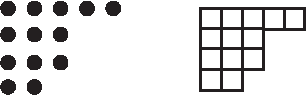
\includegraphics[width=0.33\linewidth]{images/FerrersYoung}
\caption{The Ferrers and Young diagrams of the partition (5,3,3,2)\label{FerrersYoung}}
\end{figure}
\begin{activity}[]\label{activity-86}
Draw the Young diagram of the partition (4,4,3,1,1). Describe the geometric relationship between the Young diagram of (5,3,3,2) and the Young diagram of (4,4,3,1,1).%
\par\medskip\noindent%
\textbf{Solution.}\quad \leavevmode%
\begin{figure}
\centering
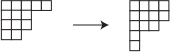
\includegraphics[width=0.33\linewidth]{images/conjugateYoung}
\caption{Forming the conjugate of a Young diagram\label{conjugateYoung}}
\end{figure}
We get the Young diagram of \((5,3,3,2)\) by flipping the Young diagram of \((4,4,3,1,1)\) around a line that includes the diagonal of the upper left box; if we think of the top left corner of the diagram as being at the origin, we flip around the line \(y=-x\).%
\end{activity}
\begin{activity}[]\label{activity-87}
The partition \((\lambda_1,\lambda_2,\ldots, \lambda_n)\) is called the \terminology{conjugate}\index{conjugate of an integer partition}\index{partition of an integer!conjugate of} of the partition \((\gamma_1,\gamma_2,\ldots, \gamma_m)\) if we obtain the Young diagram of one from the Young diagram of the other by flipping one around the line with slope -1 that extends the diagonal of the top left square. See \hyperref[conjugateYoung]{Figure~\ref{conjugateYoung}} for an example.%
\begin{figure}
\centering
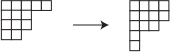
\includegraphics[width=0.5\linewidth]{images/conjugateYoung}
\caption{The Ferrers diagram the partition (5,3,3,2) and its conjugate.\label{conjugateYoung}}
\end{figure}
What is the conjugate of (4,4,3,1,1)? How is the largest part of a partition related to the number of parts of its conjugate? What does this tell you about the number of partitions of a positive integer \(k\) with largest part \(m\)?%
\par\medskip\noindent%
\textbf{Solution.}\quad \((5,3,3,2)\). The largest part of a partition equals the number of parts of its conjugate. The number of partitions of \(k\) with largest part \(m\) equals the number of partitions of \(k\) with \(m\) parts.%
\end{activity}
\begin{activity}[]\label{activity-88}
~\par
\begin{enumerate}[label=(\alph*)]
 \item A partition is called \emph{self-conjugate}\index{self-conjugate partition}\index{partition of an integer!self conjugate} if it is equal to its conjugate. Find a relationship between the number of self-conjugate partitions of \(k\) and the number of partitions of \(k\) into distinct odd parts.%
\par\medskip\noindent%
\textbf{Solution.}\quad The number of self-conjugate partitons of \(k\) equals the number of partitions of \(k\) with distinct odd parts. Here is a geometric description of a bijection from self conjugate partitions of \(k\) to partitions into distinct odd parts.%
\begin{figure}
\centering
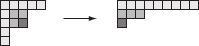
\includegraphics[width=0.33\linewidth]{images/selfconjugate}
\caption{Transforming a self-conjugate partition\label{selfconjugate-to-distinctodd}}
\end{figure}
Take the top row and left column of squares of the Young diagram, and make them into one row in a new diagram. (Only include the square that is in both the row and column once.) Now take the remaining squares in the next row and column and make a new row of the Young diagram of the second partition with them. Continue this process with succeeding rows and columns, not using any squares you have already used. Because the first partition is self conjugate, the diagram has the same number of rows as columns and row \(i\) and column \(i\) have the same length. Because row \(i\) and column \(i\) share one square, and we only use that square once when we create a new row, each row we create has odd length. Thus we get a partition with the same number of squares, so it is a partition of \(k\) and each part is odd. The parts are distinct because when we take off the squares of a row and column, we reduce the number of squares in each row and column that remains. Given a partition of \(k\) into distinct odd parts, we use the fact that each row has a unique middle element, and each is shorter than the one above (by at least two squares) to reverse the process. Thus we have a bijection.%

~\par
\item Explain the relationship between the number of partitions of \(k\) into even parts and the number of partitions of \(k\) into parts of even multiplicity, i.e. parts which are each used an even number of times as in (3,3,3,3,2,2,1,1).%
\par\medskip\noindent%
\textbf{Solution.}\quad The number of partitions of \(k\) into even parts equals the number of partitions of parts of even multiplicity, because if we take the Young diagram of a partition of \(k\) into even parts and conjugate it, the resulting diagram has columns of even length. Thus the difference in heights of two successive columns is an even number, but this difference is the multiplicity of one of the parts of the conjugate. Further the height of the last column of a partition is the multiplicity of the first part. Since the multiplicity of any part of a partition is either the difference in height of two successive columns of the Young diagram or the height of the last column, then each part of the conjugate has even multiplicity. This bijection can be reversed, because if all the differences in height of the columns are even and the height of the last column is even, then when we conjugate this partition, the last row will be an even length, and all differences in length of the rows will be even, so all the parts of the resulting partition will be even.%

\end{enumerate}
\end{activity}
\begin{activity}[]\label{rectanglecomplement}
~\par
\begin{enumerate}[label=(\alph*)]
 \item Show that the number of partitions of \(k\) into \(4\) parts equals the number of partitions of \(3k\) (or \(3k+4\) or \(3k-4\)) into \(4\) parts.%
\par\medskip\noindent%
\textbf{Solution.}\quad Think about putting the Young diagram of the partition into the upper left corner of a rectangle that is \(k\) units wide and four units high. Subdivide the rectangle into \(4k\) squares of unit area. The Young diagram covers \(k\) of these squares. The uncovered squares are in rows of length \(r_1\le r_2\le r_3\le r_4\). Thus if we list these lengths in the opposite order, we have a decreasing list representation of a partition of \(3k\). Even \(r_1\) will have to be positive, because the first part of the original partition will be at most \(k-3\). To get partitions of \(3k+4\), use a rectangle of width \(k+1\), and to get partitions of \(3k-4\), use a rectangle of width \(k-1\). Since the first row of the Young diagram has at most \(k-3\) squares, we will still have four nonzero parts in the partition that results.%

~\par
\item The idea of conjugation of a partition could be defined without the geometric interpretation of a Young diagram, but it would seem far less natural without the geometric interpretation. Another idea that seems much more natural in a geometric context is this. Suppose we have a partition of \(k\) into \(n\) parts with largest part \(m\). Then the Young diagram of the partition can fit into a rectangle that is \(m\) or more units wide (horizontally) and \(n\) or more units deep. Suppose we place the Young diagram of our partition in the top left-hand corner of an \(m'\) unit wide and \(n'\) unit deep rectangle with \(m'\ge m\) and \(n' \ge n\), as in \hyperref[complementpartition]{Figure~\ref{complementpartition}}.%
\begin{figure}
\centering
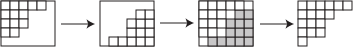
\includegraphics[width=0.33\linewidth]{images/complementpartition}
\caption{To complement the partition \((5,3,3,2)\) in a 6 by 5 rectangle: enclose it in the rectangle, rotate, and cut out the original Young diagram.\label{complementpartition}}
\end{figure}
Why can we interpret the part of the rectangle not occupied by our Young diagram, rotated in the plane, as the Young diagram of another partition? This is called the \terminology{complement}\index{complement of a partition} of our partition in the rectangle. What integer is being partitioned by the complement? What conditions on \(m'\) and \(n'\) guarantee that the complement has the same number of parts as the original one? What conditions on \(m'\) and \(n'\) guarantee that the complement has the same largest part as the original one? Is it possible for the complement to have both the same number of parts and the same largest part as the original one? If we complement a partition in an \(m'\) by \(n'\) box and then complement that partition in an \(m'\) by \(n'\) box again, do we get the same partition that we started with?%
\par\medskip\noindent%
\textbf{Solution.}\quad If we fill the rectangle with unit squares, those not in the Young diagram of the original partition \(\lambda\) will fall into rows.  The lengths of the rows are nonnegative, and are nondecreasing as we move down. Therefore, after we rotate through 180 degrees, these same rows will be listed in the opposite order, lined up along the left sides, and will have nonincreasing length. Thus they will be the Young diagram of a partition. The integer being partitioned will be \(m'n'-k\). If \(m'>m\) and \(n'=n\). the two partitions will have the same number of parts, because we will have a nonzero number of empty squares at the end of each row of the Young diagram of \(\lambda\). If \(m'=m\) and \(n'-n\) is the multiplicity of the largest part of \(\lambda\), they will have the same number of parts. Otherwise, their numbers of parts will differ. If \(n'>n\) and \(m=m'\), then the two partitions will have the same largest part. If \(n'=n\) and \(m'-m\) is the smallest part of \(\lambda\), then they will have the same largest part. Otherwise, their largest parts will differ. Thus for the two partitions to have the same number of parts, either \(m'=m\) or \(n'=n\). If \(m'=m\) and they have the same largest part, then \(n'>n\). But this is consistent with \(n'-n\) being the multiplicity of the largest part of \(\lambda\). Thus they can have the same number of parts and the same largest part if \(m'=m\) and \(n'-n\) is the multiplicity of the largest part of \(\lambda\), or similarly if \(n=n'\) and \(m'-m\) is the smallest part of \(\lambda\).%

\end{enumerate}
\end{activity}
\begin{activity}[]\label{activity-90}
~\par
\begin{enumerate}[label=(\alph*)]
 \item Suppose we take a partition of \(k\) into \(n\) parts with largest part \(m\), complement it in the smallest rectangle it will fit into, complement the result in the smallest rectangle it will fit into, and continue the process until we get the partition 1 of one into one part.  What can you say about the partition with which we started?%
\par\medskip\noindent%
\textbf{Solution.}\quad Let us call the process of enclosing \(\lambda\) in the smallest rectangle possible and then forming the complement in that rectangle \terminology{encomplementation} (This is short for \emph{en}\/closure and \emph{complementation} and is not a standard term\textemdash{}there is no standard term for this operation.) and call the result of it the \terminology{encomplement}\index{encomplement of a partition} of \(\lambda\).  The result of two encomplementations on the Young diagram of a partition is to remove all rows of maximum length and all columns of maximum length from the Young diagram. Thus the description of the result of an even number \(2j\) of encomplementations is straightforward; we remove all the rows of the \(j\) largest distinct lengths and all columns of the \(j\) largest distinct lengths. So if an even number of encomplementations brings us to a partition with one block of size one, we should be able to describe the original partition fairly easily. To deal with the result of an odd number of encomplementations, we ask what happens if we encomplement just once.  If the complement of \(\lambda\) in the smallest rectangle in which if fits has one square, then \(\lambda =\lambda_1^{n_1}\lambda_1-1\). Thus we are asking for the partitions which, after an even number of encomplementations, give us either the partition with one block or a partition of the form \(\lambda_1^{n_1}(\lambda_1-1)\). First we ask what kind of partition results in the second one after two encomplementations. If we get \(\lambda_1^{n_1}(\lambda_1-1)\) from two encomplementations, the partition we started with had the form%
\begin{equation*}
\lambda_0^{n_0}(\lambda_1+\lambda_{2})^{n_1}(\lambda_1+
\lambda_2-1)\lambda_2^{n_2}.
\end{equation*}
%
\par
If we get \(\lambda_1^{n_1}(\lambda_1-1)\) from four encomplementations, then we started with a partition of the form%
\begin{equation*}
\lambda_{-1}^{n_{-1}}(\lambda_0+\lambda_{3})^{n_0}(\lambda_1+
\lambda_2 +
\lambda_{3})^{n_1}(\lambda_1+\lambda_2 +\lambda_3-1)(\lambda_2+
\lambda_{3})^{n_3}
\lambda_3^{n_3}.
\end{equation*}
%
\par
From this pattern we see that a partition that results in \(\lambda_1^{n_1}(\lambda_1-1)\) after \(2j\) encomplementations has the form%
\begin{equation}
\lambda_{1-j}^{n_{1-j}}\lambda_{2-j}^{n_{2-j}}\cdots
\lambda_0^{n_0}
{\lambda'_1}^{n_1}
(\lambda'_1-1)\lambda_2^{n_2}\cdots
\lambda_{j+1}^{n_{j+1}},\label{form1}
\end{equation}
where \(\lambda_i>\lambda_{i+1}\) and \(\lambda_0>\lambda'_1>\lambda_2+1\).%
\par
On the other hand, a partition \(\lambda\) that results in \(1\) after two encomplementations has the form \(\lambda_0^{n_0}(\lambda_1+1)\lambda_1^{n_1}\), and so a partition that results in 1 after \(j\) encomplementations is of the form%
\begin{equation}
\lambda_{1-j}^{n_{1-j}}\lambda_{2-j}^{n_{2-j}}\cdots
\lambda_0^{n_0}(\lambda_1+1)\lambda_1^{n_1}\lambda_2^{n_2}\cdots
\lambda_j^{n_j},\label{form2}
\end{equation}
where \(\lambda_i>\lambda_{i+1}\) and \(\lambda_0>\lambda_1+1\). Thus a partition results in a single part of size 1 after some number of encomplementations if and only if it has the form of \hyperref[form1]{Equation~(\ref{form1})} or \hyperref[form2]{Equation~(\ref{form2})}.%

~\par
\item Show that \(P(k,n)\) is at least \({1\over n!}{k-1\choose n-1}\).%
\par\medskip\noindent%
\textbf{Solution.}\quad The number of compositions of \(k\) into \(n\) parts is \(k-1\choose n-1\). We can divide the compositions into blocks, where two compositions are in the same block if and only if one is a rearrangement of the other. Then the blocks correspond bijectively to partitions of \(k\) into \(n\) parts. However we cannot compute the number of blocks by dividing by the number of compositions per block since the number of compositions per block ranges from \(1\) to \(n!\).  But then if we divide the number of compositions by \(n!\) we will get a number less than the number of blocks because \(n!\) times the number of blocks would be, by the sum principle, greater than the number of partitions.%

\end{enumerate}
\end{activity}
With the binomial coefficients, with Stirling numbers of the second kind, and with the Lah numbers, we were able to find a recurrence by asking what happens to our subset, partition, or broken permutation of a set \(S\) of numbers if we remove the largest element of \(S\). Thus it is natural to look for a recurrence to count the number of partitions of \(k\) into \(n\) parts by doing something similar. Unfortunately, since we are counting distributions in which all the objects are identical, there is no way for us to identify a largest element. However if we think geometrically, we can ask what we could remove from a Young diagram to get a Young diagram. Two natural ways to get a partition of a smaller integer from a partition of \(n\) would be to remove the top row of the Young diagram of the partition and to remove the left column of the Young diagram of the partition. These two operations correspond to removing the largest part from the partition and to subtracting 1 from each part of the partition respectively. Even though they are symmetric with respect to conjugation, they aren't symmetric with respect to the number of parts. Thus one might be much more useful than the other for finding a recurrence for the number of partitions of \(k\) into \(n\) parts.%
\begin{activity}[]\label{numberpartitionrecurrence}
In this problem we will study the two operations and see which one seems more useful for getting a recurrence for \(P(k,n)\).%
~\par
\begin{enumerate}[label=(\alph*)]
 \item How many parts does the remaining partition have when we remove the largest part (more precisely, we reduce its multiplicity by one) from a partition of \(k\) into \(n\) parts?  What can you say about the number of parts of the remaining partition if we remove one from each part?%
\par\medskip\noindent%
\textbf{Solution.}\quad Reducing the multiplicity of the largest part by one reduces the number of parts by one. Removing 1 from each part reduces the number of parts by the multiplicity of the smallest part, so it strictly reduces the number of parts, perhaps even to one.%

~\par
\item If the largest part of a partition is \(j\) and we remove it, what integer is being partitioned by the remaining parts of the partition? If we remove one from each part of a partition of \(k\) into \(n\) parts, what integer is being partitioned by the remaining parts?%
\par\medskip\noindent%
\textbf{Solution.}\quad If we remove the largest part, the integer being partitioned is \(k\) minus the largest part. Thus it is a number less than \(k\) and at least \(n-1\). If we remove one from each part of the partition, the integer being partitioned is \(k-n\).%

~\par
\item The last two questions are designed to get you thinking about how we can get a bijection between the set of partitions of \(k\) into \(n\) parts and some other set of partitions that are partitions of a smaller number.  These questions describe two different strategies for getting that set of partitions of a smaller number or of smaller numbers.  Each strategy leads to a bijection between partitions of \(k\) into \(n\) parts and a set of partitions of a smaller number or numbers.  For each strategy, use the answers to the last two questions to find and describe this set of partitions into a smaller number and a bijection between partitions of \(k\) into \(n\) parts and partitions of the smaller integer or integers into appropriate numbers of parts.%
\par\medskip\noindent%
\textbf{Solution.}\quad Removing the largest part of a partition of \(k\) into \(n\) parts gives us a bijection between partitions of \(k\) into \(n\) parts and and partitions of numbers \(k'\) between \(n-1\) and \(k-1\) into \(n-1\) parts of size at most \(k-k'\). (Removing the largest part gives us such a partition, and adjoining a part of size \(k-k'\) to such a partition gives us a partition of \(k\) with \(n\) parts.)%
\par
Removing one from each part of a partition of \(k\) into \(n\) parts gives us a bijection between partitions of \(k\) into \(n\) parts and and partitions \(k-n\) into \(n\) or fewer parts. (Removing one from each part of a partition of \(k\) into \(n\) parts gives us such a partition, and, given such a partition, we get a partition of \(k\) into \(n\) parts by adding one to each part and then creating enough parts of size 1 to have \(n\) parts.)%

~\par
\item Find a recurrence (which need not have just two terms on the right hand side) that describes how to compute \(P(k,n)\) in terms of the number of partitions of smaller integers into a smaller number of parts.%
\par\medskip\noindent%
\textbf{Hint.}\quad One of the two sets of partitions of smaller numbers from the previous part is more amenable to finding a recurrence than the other.%
\par\medskip\noindent%
\textbf{Solution.}\quad The second bijection is to the set of partitions of \(k-1\) into \(n\) or fewer parts, and this makes the second bijection sound easier to work with. We get \(P(k,n)=\sum_{i=1}^n P(k-n,i)\). The proof is the bijection we already described; in particular a partition of \(k-n\) into \(i\) parts corresponds to the partition of \(k\) we get by adding one to each of the \(i\) parts and then creating \(n-i\) parts of size one.%

~\par
\item What is \(P(k,1)\) for a positive integer \(k\)?%
\par\medskip\noindent%
\textbf{Solution.}\quad \(P(k,1)=1\).%

~\par
\item What is \(P(k,k)\) for a positive integer \(k\)?%
\par\medskip\noindent%
\textbf{Solution.}\quad \(P(k,k)=1\).%

~\par
\item Use your recurrence to compute a table with the values of \(P(k,n)\) for values of \(k\) between 1 and 7.%
\par\medskip\noindent%
\textbf{Solution.}\quad \begin{tabular}{llllllll}
\(k\backslash n\)&1&2&3&4&5&6&7\tabularnewline[0pt]
&&&&&&&\tabularnewline\hrulethin
1&1&0&0&0&0&0&0\tabularnewline[0pt]
2&1&1&0&0&0&0&0\tabularnewline[0pt]
3&1&1&1&0&0&0&0\tabularnewline[0pt]
4&1&2&1&1&0&0&0\tabularnewline[0pt]
5&1&2&2&1&1&0&0\tabularnewline[0pt]
6&1&3&3&2&1&1&0\tabularnewline[0pt]
7&1&3&4&3&2&1&1
\end{tabular}

~\par
\item What would you want to fill into row 0 and column 0 of your table in order to make it consistent with your recurrence.  What does this say \(P(0,0)\) should be?  We usually define a sum with no terms in it to be zero. Is that consistent with the way the recurrence says we should define \(P(0,0)\)?%
\par\medskip\noindent%
\textbf{Solution.}\quad We would want to have \(P(0,0)=1\) and \(P(k,0)=P(0,n)=0\) for positive integer \(k\) or \(n\). Since the sum of the empty multiset of positive integers is zero, this gives us one partition of the number zero, namely the empty multiset of positive integers.%

\end{enumerate}
\end{activity}
It is remarkable that there is no known formula for \(P(k,n)\), nor is there one for \(P(k)\). This section was are devoted to developing methods for computing values of \(P(n,k)\) and finding properties of \(P(n,k)\) that we can prove even without knowing a formula. Some future sections will attempt to develop other methods.%
\par
We have seen that the number of partitions of \(k\) into \(n\) parts is equal to the number of ways to distribute \(k\) identical objects to \(n\) recipients so that each receives at least one. If we relax the condition that each recipient receives at least one, then we see that the number of distributions of \(k\) identical objects to \(n\) recipients is \(\sum_{i=1}^n P(k,i)\) because if some recipients receive nothing, it does not matter which recipients these are. This completes rows 7 and 8 of our table of distribution problems. The completed table is shown in \hyperref[lastdistributiontable]{Table~\ref{lastdistributiontable}}. There are quite a few theorems that you have proved which are summarized by \hyperref[lastdistributiontable]{Table~\ref{lastdistributiontable}}.  It would be worthwhile to try to write them all down!%
\begin{table}
\centering
\begin{tabular}{lll}
&&\tabularnewline\hrulethin
The Twentyfold Way: A Table of Distribution Problems\tabularnewline[0pt]
&&\tabularnewline\hrulemedium
\(k\) objects and conditions&\(n\) recipients and mathematical model for distribution\tabularnewline[0pt]
on how they are received&Distinct&Identical\tabularnewline[0pt]
&&\tabularnewline\hrulemedium
1.  Distinct&\(n^k\)&\(\sum_{i=1}^kS(n,i)\)\tabularnewline[0pt]
no conditions&functions&set partitions (\(\le n\) parts)\tabularnewline[0pt]
&&\tabularnewline\hrulethin
2.  Distinct&\(n^{\underline{k}}\)&1 if \(k\le n\); 0 otherwise\tabularnewline[0pt]
Each gets at most one&\kern -2pt \(k\)-element permutations\kern -2 pt&\tabularnewline[0pt]
&&\tabularnewline\hrulethin
3.  Distinct&\(S(k,n)n!\)&\(S(k,n)\)\tabularnewline[0pt]
Each gets at least one&onto functions&set partitions (\(n\) parts)\tabularnewline[0pt]
&&\tabularnewline\hrulethin
4. Distinct&\(k!=n!\)&1 if \(k=n\); 0 otherwise\tabularnewline[0pt]
Each gets exactly one&permutations&\tabularnewline[0pt]
&&\tabularnewline\hrulethin
5.  Distinct, order matters&\((k+n-1)^{\underline{k}}\)&\(\sum_{i=1}^n L(k,i)\)\tabularnewline[0pt]
&ordered functions&\hglue -3 pt broken permutations (\(\le n\) parts)\kern -3 pt\tabularnewline[0pt]
&&\tabularnewline\hrulethin
6.  Distinct, order matters&\((k)^{\underline{n}}(k-1)^{\underline{k-n}}\)&\(L(k,n)=
{ k\choose n}(k-1)^{\underline{k-n}}\)\tabularnewline[0pt]
Each gets at least one&ordered onto functions&broken permutations (\(n\) parts)\tabularnewline[0pt]
&&\tabularnewline\hrulethin
7.  Identical&\(n+k-1\choose k\)&\(\sum_{i=1}^nP(k,i)\)\tabularnewline[0pt]
no conditions&multisets&number partitions (\(\le n\) parts)\tabularnewline[0pt]
&&\tabularnewline\hrulethin
8.  Identical&\(n\choose k\)&1 if \(k\le n\); 0 otherwise\tabularnewline[0pt]
Each gets at most one&subsets&\tabularnewline[0pt]
&&\tabularnewline\hrulethin
9.  Identical&\(k-1\choose n-1\)&\(P(k,n)\)\tabularnewline[0pt]
Each gets at least one&compositions (\(n\) parts)&number partitions (\(n\) parts)\tabularnewline[0pt]
&&\tabularnewline\hrulethin
10.  Identical&1 if \(k=n\); 0 otherwise&1 if \(k=n\); 0 otherwise\tabularnewline[0pt]
Each gets exactly one&&\tabularnewline[0pt]
&&\tabularnewline\hrulethin
\end{tabular}
\caption{The number of ways to distribute \(k\) objects to \(n\) recipients, with restrictions on how the objects are received\label{lastdistributiontable}}
\end{table}
\typeout{************************************************}
\typeout{Subsection  Partitions into distinct parts}
\typeout{************************************************}
\subsection[{Partitions into distinct parts}]{Partitions into distinct parts}\label{subsection-33}
Often \(Q(k,n)\) is used to denote the number of partitions of \(k\) into distinct parts, that is, parts that are different from each other.%
\begin{activity}[]\label{activity-92}
Show that%
\begin{equation*}
Q(k,n) \le {1\over n!}{k-1\choose n-1}.
\end{equation*}
%
\par\medskip\noindent%
\textbf{Solution.}\quad The number of compositions of \(k\) into \(n\) parts is \(k-1\choose n-1\). Thus the number of compositions of \(k\) into \(n\) distinct parts is less than \(k-1\choose n-1\). Divide the compositions of \(k\) into \(n\) distinct parts into blocks with two compositions in the same block if one is a rearrangement of the other. Because the parts are distinct, each block has \(n!\) members. Further, there is a bijection between the blocks of this partition and the partitions of \(k\) into \(n\) distinct parts. Since the number of compositions of \(k\) into \(n\) distinct parts is less than \(k-1 \choose n-1\), the number of partitions of \(k\) into \(n\) distinct parts is less than \({1\over n!}  {k-1\choose n-1}\).%
\end{activity}
\begin{activity}[]\label{activity-93}
Show that the number of partitions of 7 into 3 parts equals the number of partitions of 10 into three distinct parts.%
\par\medskip\noindent%
\textbf{Solution.}\quad Given a partition \(\lambda\) of 7 in decreasing list form \(\lambda_1,\lambda_2,\lambda_3\), if we add 0 to \(\lambda_3\), \(1\) to \(\lambda_2\) and 2 to \(\lambda_1\) the resulting partition of 10 has distinct parts. If we take a partition \(\lambda'\) of 10 with distinct parts, then \(\lambda'_1\ge\lambda'_2+1\), \(\lambda'_1\ge\lambda'_2+2\), and \(\lambda'_2\ge \lambda'_3+1\). Therefore if we subtract 2 from \(\lambda'_1\) to get \(\lambda_1\), subtract 1 from \(\lambda'_2\) to get \(\lambda_2\) and let \(\lambda_3= \lambda'_3\), then \(\lambda_1,\lambda_2,\lambda_3\) is the decreasing list representation of a partition of \(10-3=7\). Thus there is a bijection between partitions of \(7\) into three parts and partitions of \(10\) into three distinct parts.%
\end{activity}
\begin{activity}[]\label{activity-94}
There is a relationship between \(P(k,n)\) and \(Q(m,n)\) for some other number \(m\). Find the number \(m\) that gives you the nicest possible relationship.%
\par\medskip\noindent%
\textbf{Solution.}\quad The number of partitions of \(k\) into \(n\) parts is equal to the number of partitions of \(k+{n\choose2}\) into n distinct parts.  The bijection from partitions of \(k\) with \(n\) parts to partitions of \(k+{n\choose2}\) with \(n\) distinct parts that proves this is the one that takes a partition \(\lambda_n\lambda_{n-1}\cdots\lambda_1\) of \(k\) with \(\lambda_i>\lambda_{i+1}\) and adds \(i-1\) to \(\lambda_i\) to get \(\lambda'_i\). Then \(\lambda'\) is a partition into distinct parts, and the number it partitions is \(k+1+2+\cdots+n-1=k+{n\choose 2}\). The proof that it is a bijection is the fact that subtracting \(n-i\) from the \(i\)\/th part of a partition of \(k\) into distinct parts yields a partition of \(k\), because part \(i+j\) is at least \(j\) smaller than part \(i\).%
\end{activity}
\begin{activity}[]\label{activity-95}
Find a recurrence that expresses \(Q(k,n)\) as a sum of \(Q(k-n,m)\) for appropriate values of \(m\).%
\par\medskip\noindent%
\textbf{Solution.}\quad Suppose \(\lambda\) is a partition of \(k\) into \(n\) distinct parts. Either 1 is one of those parts or not. Thus if we subtract 1 from each part, we either get a partition of \(k-n\) into \(n-1\) parts or a partition of \(k-n\) into \(n\) parts. If \(\lambda\) and \(\lambda'\) are different partitions of \(k\) into \(n\) distinct parts, they go to different partitions. Each partition of \(k-n\) into \(n-1\) parts or \(n\) parts can be gotten in this way from a corresponding partition of \(k\) into \(n\) parts. Thus we have a bijective correspondence and \(Q(k,n)=Q(k-n,n-1) +Q(k-n,n)\).%
\end{activity}
\begin{activity}[]\label{activity-96}
Show that the number of partitions of \(k\) into distinct parts equals the number of partitions of \(k\) into odd parts.%
\par\medskip\noindent%
\textbf{Solution.}\quad We start by giving a function from the set of partitions of \(k\) to the set of partitions of \(k\) with (only) odd parts. Clearly such a function cannot be one to one. Then we show that when restricted to the partitions with distinct parts it is one-to-one and onto by constructing an inverse. Given a partition \(\lambda_1^{i_1}\lambda_2^{i_2}\cdots\lambda_n^{i_n}\), write \(\lambda_i=\gamma_i2^{k_i}\), where \(\gamma_i\) is odd. (Thus \(2^{k_i}\) is the highest power of 2 that is a factor of \(\lambda_i\), so it is 1 if \(\lambda_i\) is odd.). It is possible that \(\gamma_i=\gamma_j\), for example if \(\lambda_i=36\) and \(\lambda_j=18\), then \(\gamma_i=\gamma_j=9\). We construct a new partition \(\pi\) whose parts are the numbers \(\gamma_j\) as follows: Given an odd number \(p\), let the multiplicity \(m(p)\) of \(p\) in \(\pi\) be \(\sum_{j: \gamma_j=m} 2^{k_j}\). Thus \(\sum_{p: m(p)\not=0}m(p)p = k\). Therefore, \(\pi\) is a partition of \(k\) whose parts are all odd.%
\par
Now consider a partition \(\pi\) of \(k\) whose parts are all odd. Let \(\pi=\pi_1^{r_1}\pi_2^{r_2}\cdots \pi_t^{r_t}\), with \(\pi_i>\pi_{i+1}\). (In terms of the multiplicity function \(m\), \(m(\pi_i) =r_i\), and \(\sum_{i=1}^t r_i\pi_i = k\).) We are going to write the binary expansion of each \(r_i\) as \(r_i = \sum_{j= 0}^{\lfloor \log_2 r_i\rfloor} 2^{ja_{ij}}\), where \(a_{ij}\) is 1 if \(2^j\) appears in the binary expansion of \(r_i\), and 0 otherwise. All of the numbers \(\pi_i2^{ja_{ij}}\) are distinct, because a power of two times one odd number cannot equal a power of two times another odd number. The numbers \(\pi_i2^{ja_{ij}}\) add to \(k\), so they are the parts of a partition \(\pi'\) of \(k\) into distinct parts. When we apply the function constructed in the first part of the solution to \(\pi'\), we get \(\pi\), so the correspondence between \(\pi\) and \(\pi'\) is a bijection.%
\end{activity}
\begin{activity}[]\label{activity-97}
Euler showed that if \(k\not= {3j^2+j\over 2}\), then the number of partitions of \(k\) into an even number of distinct parts is the same as the number of partitions of \(k\) into an odd number of distinct parts. Prove this, and in the exceptional case find out how the two numbers relate to each other.%
\par\medskip\noindent%
\textbf{Solution.}\quad This solution is taken largely from the book \textsl{Introduction to Combinatorics} by Ioan Tomescu (published in London by Collet's in 1975). Tomescu calls a collection of rows in a Young diagram a ``trapezoid'' if each row contains one less cell than the row above and the number of cells in the rows above and below the trapezoid differ by two or more from the number of cells in rows of the trapezoid. Thus in (8,6,5,4,2,1) we have 3 trapezoids, the first row, the next three rows, and the last two. Since we are dealing with partitions with distinct parts, we don't have to worry about how two equal rows affect the definition of a trapezoid. We will describe a way to transform a partition with an even number of distinct parts into a partition with an odd number of distinct parts and vice versa.%
\par
First we describe a transformation on Young diagrams. Here is the first part of the description. Suppose the smallest part \(m\) of \(\lambda\) is less than or equal to the number \(j\) of rows in the top trapezoid. Suppose further that if we have only one trapezoid, then \(j>m\). Then we construct a partition with one less part by adding 1 to each of the \(m\) largest parts and discarding the part \(m\). We still have a diagram for a partition of the same integer, but now the parity of the number of parts has changed, and we \emph{may} have increased the number of trapezoids by 1. The smallest part will now be larger than the number (now \(m\)) of rows in the top trapezoid. (Notice that the construction would not work if we had only one trapezoid and \(j=m\) because we would first remove one row of the trapezoid and thus have no row to which to attach one of our squares.)%
\par
Here is the second part of the description of the transformation. Suppose now that \(m\) is larger than the number \(j\) of rows of the top trapezoid in the Young diagram. Suppose also that the Young diagram has at least two trapezoids or it has one trapezoid and \(j\ge m-2\). Take one square from each of the \(j\) rows of the top trapezoid (which is the whole diagram if there is only one trapezoid) and also add a row of \(j\) squares at the bottom of the diagram. (Since \(m>j\), this gives us a Young diagram of a partition of the same integer into distinct parts.) The parity of the number of rows has changed, and now the number of rows of the top trapezoid is at least as large as the smallest part of the partition. (Note, two previously distinct trapezoids may have joined together to form one on top.)  (Notice that if we have one trapezoid and \(j= m+1\), then the construction yields a partition with two equal parts, which is why we made the special assumption above.) Now let \(T\) be the transformation described by the two constructions above. Its domain is all Young diagrams except those with one trapezoid and \(m\le j\le m+1\). \(T^2\) is the identity, and so \(T\) is a bijection.  When restricted to partitions with an odd number of parts, \(T\) gives partitions with an even number of parts, so on its domain it gives a bijection between partitions with an even number of parts and partitions with an odd number of parts.%
\par
If \(m=j\) and the diagram has just one trapezoid, then the diagram has \(3j^2-j\over 2\) squares, and if \(m=j+1\) and the diagram has just one trapezoid, then the diagram has \(3j^2+j\over 2\) squares. Thus if \(k\ne {3j^2\pm j\over 2}\), the number of partitions of \(k\) into distinct even parts equals the number of partitions of \(k\) into distinct odd parts.%
\par
If \(k= {3j^2\pm j\over 2}\) and \(j\) is even, then there is one diagram of a partition of \(k\) that is not in the domain of the bijection and has an even number of rows, so in this case there will be one more partition with an even number of parts than with an odd number. If \(k= {3j^2\pm j\over 2}\) and \(j\) is odd, there is one diagram with an odd number of rows not in the domain and so in this case there is one more partition with an odd number of parts than with an even number. This completes the exceptional cases of the problem.%
\end{activity}
\typeout{************************************************}
\typeout{Section 2.4 Supplementary Problems}
\typeout{************************************************}
\section[{Supplementary Problems}]{Supplementary Problems}\label{section-11}
\leavevmode%
\begin{enumerate}
\item\hypertarget{li-47}{}Answer each of the following questions with \(n^k\), \(k^n\), \(n!\), \(k!\), \(n \choose k\), \(k \choose n\), \(n^{\underline{k}}\), \(k^{\underline{n}}\), \(n^{\overline{k}}\), \(k^{\overline{n}}\), \(n+k-1\choose k\), \(n+k-1\choose n\), \(n-1\choose k-1\), \(k-1\choose n-1\), or ``none of the above". %
\begin{enumerate}
\item\hypertarget{li-48}{}In how many ways may we pass out \(k\) identical pieces of candy to \(n\) children? \(n+k-1\choose k\)%
%
\item\hypertarget{li-49}{}In how many ways may we pass out \(k\) distinct pieces of candy to \(n\) children? \(n^k\)%
%
\item\hypertarget{li-50}{}In how many ways may we pass out \(k\) identical pieces of candy to \(n\) children so that each gets at most one?  (Assume \(k\le n\).) \(n\choose k\).%
%
\item\hypertarget{li-51}{}In how many ways may we pass out \(k\) distinct pieces of candy to \(n\) children so that each gets at most one?  (Assume \(k\le n\).) \(n^{\underline{k}}\)%
%
\item\hypertarget{li-52}{}In how many ways may we pass out \(k\) distinct pieces of candy to \(n\) children so that each gets at least one?  (Assume \(k\ge n\).) None of the above.%
%
\item\hypertarget{li-53}{}In how many ways may we pass out \(k\) identical pieces of candy to \(n\) children so that each gets at least one?  (Assume \(k\ge n\).) \(k-1\choose n-1\)%
%
\end{enumerate}
%
\item\hypertarget{li-54}{}The neighborhood betterment committee has been given \(r\) trees to distribute to \(s\) families living along one side of a street. %
\begin{enumerate}
\item\hypertarget{li-55}{}In how many ways can they distribute all of them if the trees are distinct, there are more families than trees, and each family can get at most one? \(s^{\underline{r}}\)%
%
\item\hypertarget{li-56}{}In how many ways can they distribute all of them if the trees are distinct, any family can get any number, and a family may plant its trees where it chooses? \(s^r\)%
%
\item\hypertarget{li-57}{}In how many ways can they distribute all the trees if the trees are identical, there are no more trees than families,   and any family receives at most one? \(s\choose r\)%
%
\item\hypertarget{li-58}{}In how many ways can they distribute them if the trees are distinct, there are more trees than families, and each family receives at most one (so there could be some leftover trees)? \(\sum_{k=0}^s {s\choose k}r^{\underline{k}}\) or\(\sum_{k=0}^s s^{\underline{k}}{r\choose k}\)%
%
\item\hypertarget{multisetproblem}{}In how many ways can they distribute all the trees if they are identical and anyone may receive any number of trees? \(r+s-1\choose r\)%
%
\item\hypertarget{orderedfunctionproblem}{}In how many ways can all the trees be distributed and planted if the trees are distinct, any family can get any number, and a family must plant its trees in an evenly spaced row along the road? \(s^{\overline{r}}=(r+s-1)^{\underline{r}}\)%
%
\item\hypertarget{li-61}{}Answer the question in \hyperlink{orderedfunctionproblem}{Part~2.f} assuming that every family must get a tree. \(r!{r-1\choose s-1}\)%
%
\item\hypertarget{li-62}{}Answer the question in \hyperlink{multisetproblem}{Part~2.e} assuming that each family must get at least one tree. \(r-1\choose s-1\)%
%
\end{enumerate}
%
\item\hypertarget{li-63}{}In how many ways can \(n\) identical chemistry books, \(r\) identical mathematics books, \(s\) identical physics books, and \(t\) identical astronomy books be arranged on three bookshelves? (Assume there is no limit on the number of books per shelf.) \({(n+r+s+t+2)! \over n!r!s!t!2!}\)%
%
\item\hypertarget{li-64}{}(interesting) One formula for the Lah numbers is%
\begin{equation*}
L(k,n) = {k\choose n}(k-1)^{\underline{k-n}}
\end{equation*}
Find a proof that explains this product. First choose the \(n\) elements which will be the first member of the part they lie in. (This, in effect, labels the \(n\) parts.) Then assign the remaining \(k-n\) elements to their parts by making an ordered function of \(n-k\) objects to \(n\) recipients in \((n + (k-n) - 1)^{{k-n}} = (k-1)^{{k-n}}\) ways.%
%
\item\hypertarget{li-65}{}What is the number of partitions of \(n\) into two parts? \(n/2\) if \(n\) is even and \((n-1)/2\) if \(n\) is odd, equivalently, \(\lfloor n/2\rfloor\)%
%
\item\hypertarget{li-66}{}Show that the number of partitions of \(k\) into \(n\) parts of size at most \(m\) equals the number of partitions of \(mn-k\) into no more than \(n\) parts of size at most \(m-1\). If we take the complement of the Young diagram of a partition of \(k\) into \(n\) parts of size at most \(m\) in an rectangle with \(n\) rows and \(m\) columns, the number we partition will be \(mn-k\), and we will have no more than \(n\) parts, each of size at most \(m-1\). And if we take the complement of a partition of this second kind in the same rectangle, we will get a partition of the first kind.%
%
\item\hypertarget{li-67}{}Show that the number of partitions of \(k\) into parts of size at most \(m\) is equal to the number of partitions of of \(k+m\) into \(m\) parts. Given the first kind of partition, take the conjugate (giving a partition of \(k\) into at most \(m\) parts), add one to each part, and then add enough parts of size 1 to get a total of \(m\) parts. It is straightforward that this process can be reversed.%
%
\item\hypertarget{li-68}{}You can say something pretty specific about self-conjugate partitions of \(k\) into distinct parts.  Figure out what it is and prove it.  With that, you should be able to find a relationship between these partitions and partitions whose parts are consecutive integers, starting with 1.  What is that relationship? In a self-conjugate partition, the number of parts is the size of the largest part. If these parts are distinct, this means that each number between 1 and the largest part appears once as a part. That is, the parts are a list of consecutive integers, starting with 1.%
%
\item\hypertarget{li-69}{}What is \(s(k,1)\)? Since s\((k,1)\) is the coefficient of \(x^1\) in%
\begin{equation*}
x^{\underline{k}} = x(x-1)
(x-2)\cdot (x-(k-1)),
\end{equation*}
it is \((-1)^{k-1}(k-1)!\).%
%
\item\hypertarget{li-70}{}Show that the Stirling numbers of the second kind satisfy the recurrence%
\begin{equation*}
S(k,n) = \sum_{i=1}^kS(k-i,n-1){n-1\choose i-1}.
\end{equation*}
A partition of \([k]\) into \(n\) blocks has a block containing \(k\). If this block has size \(i\), when you remove it, you get a partition of a set of size \(k-i\) into \(n-1\) blocks. The number of possible sets of size \(i\) containing \(k\) is \(k-1\choose i-1\), and \(i\) can be any number between 1 and \(k\). Each partition of \(k\) into \(n\) blocks may be constructed exactly once by first choosing the block containing \(k\) and then partitioning the remaining elements into \(n-1\) blocks. This proves the formula.%
%
\item\hypertarget{li-71}{}(interesting) Let \(c(k,n)\) be the number of ways for \(k\) children to hold hands to form \(n\) circles, where one child clasping his or her hands together and holding them out to form a circle is considered a circle.  Find a recurrence for \(c(k,n)\).  Is the family of numbers \(c(k,n)\) related to any of the other families of numbers we have studied? If so, how? The \(k\)th child is either in a circle by him/her self, and there are \(c(k-1,n-1)\) ways for this to happen, or is in a circle with some other children. In the second case child \(i\) can be to the immediate right of any of the other \(k-1\) children, so there are \((k-1)c(k-1,n)\) ways for this to happen. Thus \(c(k,n)=c(k-1,n-1)
+(k-1)c(k-1,n)\). This recurrence is almost the same as the recurrence for \(s(k,n)\), except it has a plus sign where the recurrence for the Stirling numbers of the first kind has a minus sign. Further \(c(k,1)=(k-1)!\) and \(c(k,k)=1\), which agrees, except for sign, with the Stirling numbers of the first kind. If we experiment with applying the recurrence, we see that whenever we use it to compute \(c(k,n)\), we get that \(c(k,n)=|s(k,n)|\). It is now straightforward to prove by induction that \(c(k,n)=|s(k,n)|\).%
%
\end{enumerate}
\typeout{************************************************}
\typeout{Chapter 3 The Principle of Inclusion and Exclusion}
\typeout{************************************************}
\chapter[{The Principle of Inclusion and Exclusion}]{The Principle of Inclusion and Exclusion}\label{chapter-4}
\typeout{************************************************}
\typeout{Section 3.1 The Principle of Inclusion and Exclusion}
\typeout{************************************************}
\section[{The Principle of Inclusion and Exclusion}]{The Principle of Inclusion and Exclusion}\label{sec_inclexcl-inclexcl}
\typeout{************************************************}
\typeout{Subsection  The size of a union of sets}
\typeout{************************************************}
\subsection[{The size of a union of sets}]{The size of a union of sets}\label{subsection-34}
One of our very first counting principles was the \emph{sum principle}\index{sum principle} which says that the size of a union of disjoint sets is the sum of their sizes. Computing the size of overlapping sets requires, quite naturally, information about how they overlap. Taking such information into account will allow us to develop a powerful extension of the sum principle known as the ``principle of inclusion and exclusion.''\index{principle of inclusion and exclusion}\index{inclusion and exclusion principle}%
\begin{activity}[]\label{fertilizer2}
In a biology lab study of the effects of basic fertilizer ingredients on plants, 16 plants are treated with potash, 16 plants are treated with phosphate, and among these plants, eight are treated with both phosphate and potash. No other treatments are used. How many plants receive at least one treatment? If 32 plants are studied, how many receive no treatment?%
\par\medskip\noindent%
\textbf{Solution.}\quad The number of plants receiving treatment was \(16+16-8 = 24\). The number of plants receiving no treatment was eight.%
\end{activity}
\begin{activity}[]\label{activity-99}
Give a formula for the size of the union \(A\cup B\) of two sets \(A\) in terms of the sizes \(|A|\) of \(A\), \(|B|\) of \(B\), and \(|A\cap B|\) of \(A\cap B\). If \(A\) and \(B\) are subsets of some ``universal'' set \(U\), express the size of the complement \(U-(A\cup B)\) in terms of the sizes \(|U|\) of \(U\), \(|A|\) of \(A\), \(|B|\) of \(B\), and \(|A\cap B|\) of \(A\cap B\).%
\par\medskip\noindent%
\textbf{Solution.}\quad \(|A\cup B|=|A| + |B| - |A\cap B|\).%
\par
\(|U-(A\cup B)| = |U|-|A|-|B| + |A
\cap B|\).%
\end{activity}
\begin{activity}[]\label{activity-100}
In \hyperref[fertilizer2]{Problem~\ref{fertilizer2}}, there were just two fertilizers used to treat the sample plants. Now suppose there are three fertilizer treatments, and 15 plants are treated with nitrates, 16 with potash, 16 with phosphate, 7 with nitrate and potash, 9 with nitrate and phosphate, 8 with potash and phosphate and 4 with all three. Now how many plants have been treated? If 32 plants were studied, how many received no treatment at all?%
\par\medskip\noindent%
\textbf{Solution.}\quad \(15+16+16-7-9-8+4=27\) plants were treated and five received no treatment.%
\end{activity}
\begin{activity}[]\label{threesetintersection}
Give a formula for the size of \(A_1\cup A_2\cup A_3\) in terms of the sizes of \(A_1\), \(A_2\), \(A_3\) and the intersections of these sets.%
\par\medskip\noindent%
\textbf{Solution.}\quad \(|A\cup B\cup C|=|A|+|B|+|C|-|A\cap B|- |A\cap C| - |B\cap
C| +|A\cap B\cap C|\).%
\end{activity}
\begin{activity}[]\label{nsetintersection}
Conjecture a formula for the size of a union of sets%
\begin{equation*}
A_1\cup
A_2\cup \cdots\cup A_n = \bigcup_{i=1}^n A_i
\end{equation*}
in terms of the sizes of the sets \(A_i\) and their intersections.%
\par\medskip\noindent%
\textbf{Solution.}\quad %
\begin{equation*}
\left|\bigcup_{i=1}^n A_i\right| = \sum_{i=1}^n|A_i| -
\sum_{i=1}^n\sum_{j=i+1}^n |A_i \cap A_j| + \cdots +(-1)^{n-1} |A_1\cap
A_2\cap\cdots \cap A_n|.
\end{equation*}
\end{activity}
The difficulty of generalizing \hyperref[threesetintersection]{Problem~\ref{threesetintersection}} to \hyperref[nsetintersection]{Problem~\ref{nsetintersection}} is not likely to be one of being able to see what the right conjecture is, but of finding a good notation to express your conjecture. In fact, it would be easier for some people to express the conjecture in words than to express it in a notation. Here is some notation that will make your task easier. Let us define%
\begin{equation*}
\bigcap_{i:i\in I}A_i
\end{equation*}
to mean the intersection over all elements \(i\) in the set \(I\) of \(A_i\). Thus%
\begin{equation}
\bigcap_{i:i\in
\{1,3,4,6\}} = A_1\cap A_3\cap A_4 \cap A_6.\label{intersectionnotation}
\end{equation}
%
\par
This kind of notation, consisting of an operator with a description underneath of the values of a dummy variable of interest to us, can be extended in many ways. For example%
\begin{align*}
\sum_{I:I \subseteq \{1,2,3,4\}, \ |I|=2} |\cap_{i\in I}
A_i| \amp =\amp  |A_1\cap A_2|+ |A_1\cap A_3|
+|A_1\cap A_4|\nonumber\\
\amp +\amp  |A_2\cap A_3|+
|A_2\cap A_4| +|A_3\cap A_4|.
\end{align*}
%
\begin{activity}[]\label{inclusion-exclusionunion}
Use notation something like that of \hyperref[intersectionnotation]{Equation~(\ref{intersectionnotation})} and {$\langle\langle$Unresolved xref, reference "notationsolution"; check spelling or use "provisional" attribute$\rangle\rangle$} to express the answer to \hyperref[nsetintersection]{Problem~\ref{nsetintersection}}. Note there are many different correct ways to do this problem. Try to write down more than one and choose the nicest one you can. Say why you chose it (because your view of what makes a formula nice may be different from somebody else's). The nicest formula won't necessarily involve all the elements of \hyperref[intersectionnotation]{Equations~(\ref{intersectionnotation})} and {$\langle\langle$Unresolved xref, reference "notationsolution"; check spelling or use "provisional" attribute$\rangle\rangle$}.%
\par\medskip\noindent%
\textbf{Solution.}\quad %
\begin{equation*}
\left|\bigcup_{i=1}^n A_i\right| = \sum_{S:S\subseteq [n],
S\not=\emptyset}(-1)^{|S|-1}|\bigcap_{i: i\in S}A_i|
\end{equation*}
I chose this way of writing the formula partly because it is efficient with symbols; for example, it uses only one sum sign. But more importantly I chose it because it captures what I would want to say in words: ``You sum, over all ways of choosing an intersection of the sets \(A_i\), the size of the intersection times a sign factor that is -1 if you are intersecting an even number of sets and 1 if you are intersecting an odd number." If I were writing my solution out in words, I would probably assume that nobody would think about the possibility of an intersection of the empty set of the \(A_i\)s, but I had to put the \(S\not=\emptyset\) in my formula because otherwise the formula would have had us consider the possibility that \(S\) was empty.%
\end{activity}
\begin{activity}[]\label{hatcheck}
A group of \(n\) students goes to a restaurant carrying backpacks. The manager invites everyone to check their backpack at the check desk and everyone does. While they are eating, a child playing in the check room randomly moves around the claim check stubs on the backpacks. What is the probability that, at the end of the meal, at least one student receives his or her own backpack? In other words, in what fraction of the total number of ways to pass the backpacks back does at least one student get his or her own backpack back? (Hint: For each student, how big is the set of backpack distributions in which that student gets the correct backpack? It might be a good idea to first consider cases with \(n=3\), 4, and 5.) What is the probability that no student gets his or her own backpack?%
\par\medskip\noindent%
\textbf{Solution.}\quad First we compute the number of ways to pass out the backpacks so that at least one student gets the correct one, then we divide by \(n!\) the total number of ways to pass out the backpacks to get the probability that at least one student gets the correct one. If we let \(A_i\) be the set of backpack distributions in which student \(i\) gets the correct backpack, then the number we want to compute is the size of the union of the sets \(A_i\). For this purpose we need to know, for every subset \(S\subseteq [n]\) the size of \(\cap_{i\in S}A_i\). That is, we need to know the number of ways to pass out the backpacks so that student \(i\) gets the correct one for each \(i\) in \(S\). It won't matter whether or not other students get the correct backpacks, so we can just assume that for each \(i\in S\), student \(i\) gets the correct backpack and then hand out the remaining \(n-|S|\) backpacks to the remaining \(n-|S|\) students in \((n-|S|)!\) ways. Thus \((n-|S|)!\) is \(|\cap_{i:i\in S}A_i|\). Using our formula from \hyperref[inclusion-exclusionunion]{Problem~\ref{inclusion-exclusionunion}} we get%
\begin{align*}
\left|\bigcup_{i=1}^n A_i \right| \amp =\amp  \sum_{S:
S\subseteq [n], S\not=\emptyset}
(-1)^{|S|-1}\left|\bigcap_{i:i\in S} A_i \right|\\
\amp =\amp \sum_{S:
S\subseteq [n], S\not=\emptyset}(-1)^{|S|-1} (n-|S|)!\\
\amp =\amp
\sum_{s=1}^n {n\choose
s}(-1)^{s-1}(n-s)!\\
\amp =\amp \sum_{s=1}^n
(-1)^{s-1}{n!\over s!}
\end{align*}
%
\par
Dividing this by \(n!\), the total number of ways to pass back the backpacks, we get \(\displaystyle \sum_{s=1}^n {(-1)^{s-1}\over s!}\) for the probability that at least one student gets the correct backpack. Subtracting from 1 to get the probability that no student gets the correct backpack gives us%
\begin{equation*}
1- \sum_{s=1}^n {(-1)^{s-1}\over
s!}=\sum_{s=0}^n{(-1)^s\over s!}.
\end{equation*}
%
\end{activity}
\begin{activity}[]\label{activity-105}
As the number of students becomes large, what does the probability that no student gets the correct backpack approach?%
\par\medskip\noindent%
\textbf{Solution.}\quad From calculus, we know that \(e^x=\sum_{j=0}^\infty {x^j\over
j!}\). Substituting \(x=-1\) gives us \(e^{-1}=\sum_{j=0}^\infty
{(-1)^j\over j!}\) which is the limit as \(n\) becomes infinite of the probability in the solution to \hyperref[hatcheck]{Problem~\ref{hatcheck}}. Thus the probability approaches \(1/e\).%
\end{activity}
The formula you have given in \hyperref[inclusion-exclusionunion]{Problem~\ref{inclusion-exclusionunion}} is often called \emph{the principle of inclusion and exclusion}\index{inclusion and exclusion principle!for unions of sets}\index{principle of inclusion and exclusion!for unions of sets} for unions of sets. The reason is the pattern in which the formula first adds (includes) all the sizes of the sets, then subtracts (excludes) all the sizes of the intersections of two sets, then adds (includes) all the sizes of the intersections of three sets, and so on. Notice that we haven't yet proved the principle. We will first describe the principle in an apparently more general situation that doesn't require us to translate each application into the language of sets. While this new version of the principle might seem more general than the principle for unions of sets; it is equivalent. However once one understands the notation used to express it, it is more convenient to apply.%
\par
\hyperref[hatcheck]{Problem~\ref{hatcheck}} is ``classically'' called the \emph{hatcheck problem}\index{hatcheck problem}; the name comes from substituting hats for backpacks. If is also sometimes called the \emph{derangement problem}\index{derangement problem}. A \emph{derangement}\index{derangement} of an \(n\)-element set is a permutation of that set (thought of as a bijection) that maps no element of the set to itself. One can think of a way of handing back the backpacks as a permutation \(f\) of the students: \(f(i)\) is the owner of the backpack that student \(i\) receives. Then a derangement is a way to pass back the backpacks so that no student gets his or her own.%
\typeout{************************************************}
\typeout{Subsection  The hatcheck problem restated}
\typeout{************************************************}
\subsection[{The hatcheck problem restated}]{The hatcheck problem restated}\label{subsection-35}
The last question in \hyperref[hatcheck]{Problem~\ref{hatcheck}} requires that we compute the number of ways to hand back the backpacks so that nobody gets his or her own backpack. We can think of the set of ways to hand back the backpacks so that student \(i\) gets the correct one as the set of permutations of the backpacks with the property that student \(i\) gets his or her own backpack. Since there are \(n-1\) other students and they can receive any of the remaining \(n-1\) backpacks in \((n-1)\) ways, the number of permutations with the property that student \(i\) gets the correct backpack is \((n-1)!\). How many permutations are there with the properties that student \(i\) gets the correct backpack \emph{and} student \(j\) gets the correct backpack? (Let's call these properties \(i\) and \(j\) for short.) Since there are \(n-2\) remaining students and \(n-2\) remaining backpacks, the number of permutations with properties \(i\) and \(j\) is \((n-2)!\). Similarly, the number of permutations with properties \(i_1,i_2,\ldots,i_k\) is \((n-k)!\). Thus when we compute the size of the union of the sets%
\begin{equation*}
S_i=\{f: f\mbox{ is a permutation with property } i\},
\end{equation*}
we are computing the number of ways to pass back the backpacks so that at least one student gets the correct backpack. This answers the first question in \hyperref[hatcheck]{Problem~\ref{hatcheck}}. The last question in \hyperref[hatcheck]{Problem~\ref{hatcheck}} is asking us for the number of ways to pass back the backpacks that have \emph{none} of the properties. To say this in a different way, the question is asking us to compute the number of ways of passing back the backpacks that have exactly the \emph{empty set}, \(\emptyset\), of properties.%
\typeout{************************************************}
\typeout{Subsection  Basic counting functions: \(N_{ at least }\) and \(N_{ exactly }\)}
\typeout{************************************************}
\subsection[{Basic counting functions: \(N_{ at least }\) and \(N_{ exactly }\)}]{Basic counting functions: \(N_{ at least }\) and \(N_{ exactly }\)}\label{subsection-36}
Notice that the quantities that we were able to count easily were the number of ways to pass back the backpacks so that we satisfy a certain subset \(K= \{i_1,i_2,\ldots,i_k\}\) of our properties. In fact, among the \((n-k)\) ways to pass back the backpacks with this particular set \(K\) of properties is the permutation that gives each student the correct backpack, and has not just the properties in \(K\), but the whole set of properties. Similarly, for any set \(M\) of properties with \(K\subseteq
M\), the permutations that have all the properties in \(M\) are among the \((n-k)!\) permutations that have the properties in the set \(K\). Thus we can think of \((n-k)!\) as counting the number of permutations that have \emph{at least} the properties in \(K\). In particular, \(n!\) is the number of ways to pass back the backpacks that have at least the empty set of properties. We thus write \(N_{\mbox{at least} }(\emptyset)=n!\), or \(N_{\mbox{a} }(\emptyset)=n!\) for short. For a \(k\)-element subset \(K\) of the properties, we write \(N_{\mbox{at least} }(K) =(n-k)!\) or \(N_{\mbox{a} }(K) =(n-k)!\) for short.%
\par
The question we are trying to answer is ``How many of the distributions of backpacks have exactly the empty set of properties?" For this purpose we introduce one more piece of notation. We use \(N_{\mbox{exactly} }(\emptyset)\) or \(N_{\mbox{e} }(\emptyset)\) to stand for the number of backpack distributions with exactly the empty set of properties, and for any set \(K\) of properties we use \(N_{\mbox{exactly} }(K)\) or \(N_{\mbox{e} }(K)\) to stand for the number of backpack distributions with exactly the set \(K\) of properties. Thus \(N_{\mbox{e} }(K)\) is the number of distributions in which the students represented by the set \(K\) of properties get the correct backpacks back and no other students do.%
\typeout{************************************************}
\typeout{Subsection  The principle of inclusion and exclusion for properties}
\typeout{************************************************}
\subsection[{The principle of inclusion and exclusion for properties}]{The principle of inclusion and exclusion for properties}\label{subsection-37}
For the principle of inclusion and exclusion for properties, suppose we have a set of arrangements (like backpack distributions) and a set \(P\) of properties (like student \(i\) gets the correct backpack) that the arrangements might or might not have. We suppose that we know (or can easily compute) the numbers \(N_{\mbox{a} }(K)\) for every subset \(K\) of \(P\). We are most interested in computing \(N_{\mbox{e} }(\emptyset)\), the number of arrangements with none of the properties, but it will turn out that with no more work we can compute \(N_{\mbox{e} }(K)\) for every subset \(K\) of \(P\). Based on our answer to \hyperref[hatcheck]{Problem~\ref{hatcheck}} we expect that%
\begin{equation}
N_{\mbox{e} }(\emptyset) = \sum_{S: S\subseteq P} (-1)^{|S|}N_{\mbox{a} }(S)\label{incexempty}
\end{equation}
and it is a natural guess that, for every subset \(K\) of \(S\),%
\begin{equation}
N_{\mbox{e} }(K) = \sum_{S: K\subseteq S\subseteq P}
(-1)^{|S|-|K|}N_{\mbox{a} }(S).\label{incexnonempty}
\end{equation}
%
\par
\hyperref[incexempty]{Equations~(\ref{incexempty})} and \hyperref[incexnonempty]{Equation~(\ref{incexnonempty})} are called \emph{the principle of inclusion and exclusion for properties}.\index{inclusion and exclusion principle!for properties}\index{principle of inclusion and exclusion!for properties}%
\begin{activity}[]\label{activity-106}
Verify that the formula for the number of ways to pass back the backpacks in \hyperref[hatcheck]{Problem~\ref{hatcheck}} so that nobody gets the correct backpack has the form of \hyperref[incexempty]{Equation~(\ref{incexempty})}.%
\par\medskip\noindent%
\textbf{Solution.}\quad Suppose we take property \(i\) to be the property that student \(i\) gets the correct backpack. In our solution to \hyperref[hatcheck]{Problem~\ref{hatcheck}} we thought of \(S\) as a subset of \([n]\). Since we are numbering our properties from \(1\) to \(n\), each set \(S\) determines a corresponding set \(S'\) of properties: those properties numbered by the elements of \(S\). We will use \(P\) to stand for the set of all properties, that is property 1 through property \(n\). The number of ways to pass back the hats so that nobody gets the correct hat is \(n!\) minus the number of ways to pass back the hats so that somebody does get the correct hat back. From our solution to \hyperref[hatcheck]{Problem~\ref{hatcheck}}, we see that one way to express this is as%
\begin{align*}
n!-\sum_{S:
S\subseteq [n], S\not=\emptyset}(-1)^{|S|-1} (n-|S|)!\amp =\amp
n!+\sum_{S:
S\subseteq [n], S\not=\emptyset}(-1)^{|S|} (n-|S|)!\\
\amp =\amp
\sum_{S:
S\subseteq [n]}(-1)^{|S|} (n-|S|)!\\
\amp =\amp \sum_{S:
S\subseteq [n]}(-1)^{|S|} N_{\mbox{a} }(S')\\
\amp =\amp
\sum_{S':
S'\subseteq P}(-1)^{|S|} N_{\mbox{a} }(S')
\end{align*}
because \(N_{\mbox{a} }(S')\) is the number of ways to pass back the backpacks so that at least the students in \(S\) get the correct backpacks, which is the same as the size of \(\bigcap_{i:i\in S} A_i\), and which we computed to be \((n-|S|)!\).%
\end{activity}
\begin{activity}[]\label{incexsystemeq}
Find a way to express \(N_{\mbox{a} }(S)\) in terms of \(N_{\mbox{e} }(J)\) for subsets \(J\) of \(P\) containing \(S\). In particular, what is the equation that expresses \(N_{\mbox{a} }(\emptyset)\) in terms of \(N_{\mbox{e} }(J)\) for subsets \(J\) of \(P\)?%
\par\medskip\noindent%
\textbf{Solution.}\quad \(N_{\mbox{a} }(S) = \sum_{J: S\subseteq
J\subseteq P}N_{\mbox{e} }(J)\). In particular, we get by substitution that \(N_{\mbox{a} }(\emptyset)=\sum_{J:J\subseteq P} N_{\mbox{e} }(J)\).%
\end{activity}
\begin{activity}[]\label{activity-108}
~\par
\begin{enumerate}[label=(\alph*)]
 \item Substitute the formula for \(N_{\mbox{a} }\) from \hyperref[incexsystemeq]{Problem~\ref{incexsystemeq}} into the right hand sides of the formulas of \hyperref[incexempty]{Equations~(\ref{incexempty})} and \hyperref[incexnonempty]{Equation~(\ref{incexnonempty})} and simplify what you get to show that for \hyperref[incexempty]{Equations~(\ref{incexempty})} and \hyperref[incexnonempty]{Equation~(\ref{incexnonempty})} the right-hand sides are indeed equal to the left-hand sides. This will prove that those equations are true. (Hint: You will get a double sum. If you can figure out how to reverse the order of the two summations, the binomial theorem may help you simplify the formulas you get.)%
\par\medskip\noindent%
\textbf{Solution.}\quad Since \hyperref[incexempty]{Equation~(\ref{incexempty})} is a special case of \hyperref[incexnonempty]{Equation~(\ref{incexnonempty})}, we will just substitute the formula from \hyperref[incexsystemeq]{Problem~\ref{incexsystemeq}} into the right-hand side of \hyperref[incexnonempty]{Equation~(\ref{incexnonempty})}. This gives us%
\begin{align*}
\hspace{-.25 in}\sum_{S: K\subseteq S\subseteq P}
(-1)^{|S|-|K|}N_{\mbox{a} }(S)\amp =\amp \sum_{S: K\subseteq S\subseteq P}
(-1)^{|S|-|K|}\sum_{J: S\subseteq
J\subseteq P}N_{\mbox{e} }(J)\\
\amp =\amp \sum_{S: K\subseteq S\subseteq P}
\sum_{J: S\subseteq
J\subseteq P}(-1)^{|S|-|K|}N_{\mbox{e} }(J)\\
\amp =\amp \sum_{J:K\subseteq J\subseteq P}\sum_{S:K\subseteq S\subseteq J}
(-1)^{|S|-|K|}N_{\mbox{e} }(J)\\
\amp =\amp \sum_{J:K\subseteq J\subseteq P}N_{\mbox{e} }(J)\sum_{S:K\subseteq
S\subseteq J} (-1)^{|S|-|K|}\\
\amp =\amp \sum_{J:K\subseteq J\subseteq P}N_{\mbox{e} }(J)\sum_{s=|K|}^{|J|}
{|J|-|K|
\choose s-|K|}(-1)^{s-|K|}\\
\amp =\amp \sum_{J:K\subseteq J\subseteq P}N_{\mbox{e} }(J)\sum_{i=0}^{|J|-|K|}
{|J|-|K|
\choose i}(-1)^{i}\\
\amp =\amp \sum_{J:K\subseteq J\subseteq
P}N_{\mbox{e} }(J)(1-1)^{|J|-|K|}\\
\amp =\amp N_{\mbox{e} }(K).
\end{align*}
%
\par
In the fourth-to-last line of our equations, we used the fact that the number of subsets \(S\) of \(J\) that contain \(K\) is the number of ways to choose the elements of the set \(S-K\) of elements in \(S\) but not \(K\) from the elements of \(J-K\), the set of elements of \(J\) that are not in \(K\). In the second-to-last line of the equations, we recognized that the second sum in the third-to-last line is the kind of sum we would get by applying the binomial theorem to something of the form \((x+y)^{|J|-|K|}\) for a suitable \(x\) and \(y\), and then saw that \(x=1\) and \(y=-1\) would give us exactly the second sum in the third-to-last line. In going from the second-to-last line to the last line we used the facts that \(0^n=o\) if \(n>0\) and \(0^0=1\). This proves that \hyperref[incexnonempty]{Equation~(\ref{incexnonempty})} is true for all \(K\), and in particular when \(K=\emptyset\), which also proves \hyperref[incexempty]{Equation~(\ref{incexempty})}. We have just proved the Principle of inclusion and exclusion.%

~\par
\item In how many ways may we distribute \(k\) identical apples to \(n\) children so that no child gets more than three apples?%
\par\medskip\noindent%
\textbf{Solution.}\quad Let property \(i\) be ``Child \(i\) gets four or more apples.'' Then we are asking for the number of ways to pass out the apples that have none of the properties, so we are asking for \(N_{\mbox{e} }(\emptyset)\). From \hyperref[incexempty]{Equation~(\ref{incexempty})} we see that to find this number we need to know \(N_{\mbox{a} }(S)\) for every subset \(S\) of our set of properties. But if \(S\) has size \(s\), then having the properties in \(S\) means that all the children in a particular set of size \(s\) will get four or more apples. We already know how to pass out the apples so that the children in a particular set \(\hat S\) of children get at least four apples: we give everyone in \(\hat
S\) four apples, and then pass out the remaining \(k-4s\) apples to the children in \({k-4s+n-1\choose k-4s}= {k-4s+n-1\choose n-1}\) ways. This counts the number of ways to give at least four apples to every child in \(\hat S\), and maybe give four apples to some other children as well. Thus \(N_{\mbox{a} }(S) = {k-4|S|+n-1\choose n-1}\). Applying \hyperref[incexempty]{Equation~(\ref{incexempty})} gives us%
\begin{align*}
N_{\mbox{e} }(\emptyset)\amp =\amp \sum_{S:S\subseteq
P}(-1)^{|S|}N_{\mbox{a} }(S)\\
\amp =\amp \sum_{s=0}^k {k\choose s}(-1)^s {k-4s+n-1\choose n-1}\\
\amp =\amp \sum_{s=0}^k (-1)^s{k\choose s}{k-4s+n-1\choose n-1}
\end{align*}
%

\end{enumerate}
\end{activity}
\begin{activity}[]\label{relaxedmenage}
A group of \(n\) married couples comes to a group discussion session where they all sit around a round table. In how many ways can they sit so that no person is next to his or her spouse? (Note that two people of the same sex can sit next to each other.)%
\par\medskip\noindent%
\textbf{Solution.}\quad Let Property \(i\) be that couple \(i\) sits together. We are interested in the number of seating arrangements that have none of the properties. Thus for a set \(S\) of properties, we need to compute \(N_{\mbox{a} }(S)\). If we let each couple described by \(S\) sit together, we will seat \(|S|\) couples and \(2n-2|S|\) individuals around the table. We can do this in \(2^{|S|}(|S| + 2n-2 |S|-1)!\) ways, because once we chose a place for a couple (i.e. two adjacent seats) there are two ways the couple can sit down. Thus \(N_{\mbox{a} }(S) =2^{|S|}(2n-|S|-1)!\). Substituting this into \hyperref[incexempty]{Equation~(\ref{incexempty})} with \(P\) as the set of all properties gives us%
\begin{align*}
N_{\mbox{e} }(\emptyset) \amp =\amp  \sum_{S:S\subseteq P}
(-1)^{|S|} N_{\mbox{a} }(S)\\
\amp =\amp \sum_{s=0}^n(-1)^s{n\choose s}2^{s}(2n- s-1)!
\end{align*}
%
\end{activity}
\begin{activity}[]\label{activity-110}
A group of \(n\) married couples comes to a group discussion session where they all sit around a round table. In how many ways can they sit so that no person is next to his or her spouse or a person of the same sex? This problem is called the \emph{menage problem}.\index{menage problem} (Hint: Reason somewhat as you did in \hyperref[relaxedmenage]{Problem~\ref{relaxedmenage}}, noting that if the set of couples who do sit side-by-side is nonempty, then the sex of the person at each place at the table is determined once we seat one couple in that set.)%
\par\medskip\noindent%
\textbf{Solution.}\quad We are going to consider arrangements of the couples alternating sex around the table. Property \(i\) of an arrangement is that couple \(i\) sits together. We are interested in the number of arrangements that have exactly none of the properties. Thus for each subset \(S\) of the properties, we consider the number of arrangements that has at least the set \(S\) of properties. We distinguish the case that \(S\) is empty from the others. \(N_{\mbox{a} }(\emptyset)\) is just the number of ways to seat \(2n\) couples around the table, alternating sex, but with no other restrictions. We can arrange one of the sexes in a circle in \(n-1!\) ways and then assign the members of the opposite sex to the places between them in \(n!\) ways, so \(N_{\mbox{a} }(\emptyset) = (n-1)!n!\). (Another way to get this result is to let one person sit down. This determines the sex of the person at each place of the table, so there are \((n-1)!\) ways to assign the people of the same sex of the first person, and \(n!\) ways to assign the people of the opposite. It appears that there are \(2n\) choices for where the first person sits, but we can break the seating charts up into blocks of \(2n\) seating charts, each of which gives the same circular arrangement. Thus there are \((n-1)!n!\) inequivalent ways to seat the people with at least the empty set of properties.)%
\par
Now if \(S\) is nonempty, and has \(s\) members, we seat one of the couples that must sit together (say the first in alphabetical order), and this determines the sex of the person that must sit at each other place. There are \(2n\) pairs of adjacent seats where we can seat that couple and two ways they can sit in the pair of adjacent seats that we choose. Then we have \(s-1\) couples, \(n-s\) men and \(n-s\) women to seat in the remaining places. First we arrange the \(s-1\) couples and \(2n-2s\) identical empty chairs in places at the table in \((2n-2s+s-1)!/(2n-2s)!=(2n-s-1)!/(2n-2s)!\) ways. Each couple can sit in only one way in the places they have chosen, because the sex of the person in a given place has been determined by how the first couple sits. The sex of the person in each of the remaining chairs has been determined, so we assign the men to their seats in \((n-s)!\) ways and we assign the women to their seats in \((n-s)!\) ways. Thus we have \(2\cdot2n(2n-s-1)!(n-s)!^2/(2n-2s)!\) ways to place the people. But we can partition the placements into blocks of \(2n\) equivalent placements, because shifting everyone the same number of places to the right or left gives an equivalent placement. Thus the number of inequivalent seating arrangements is%
\begin{align*}
{2(2n-s-1)!(n-s)!^2\over(2n-2s)!}\amp =\amp {2(2n-s-1)!(n-s)!^2\over
2(n-s)(2n-2s-1)!}\\
\amp =\amp {(2n-s-1)!(n-s)!(n-s-1)!\over(2n-2s-1)!}.
\end{align*}
%
\par
Notice that if we take \(s=0\), this formula reduces to \((n-1)!n!\). Thus for all sets \(S\)%
\begin{equation*}
N_{\mbox{a} }(S)={(2n-s-1)!(n-s)!(n-s-1)!\over(2n-2s-1)!}.
\end{equation*}
%
\par
Then from \hyperref[incexempty]{Equation~(\ref{incexempty})}%
\begin{align*}
N_{\mbox{e} } \amp =\amp  \sum_{S:S\subseteq P} (-1)^{|S|}{(2n-|S|-1)!(n-|S|)!(n-|S|-1)!
\over(2n-2|S|-1)!}\\
\amp =\amp \sum_{s=0}^n(-1)^s{n\choose s}{(2n-s-1)!(n-s)!(n-s-1)!\over(2n-2s-1)!}\\
\amp =\amp \sum_{s=0}^n(-1)^s{n!\over
s!(n-s)!}{(2n-s-1)!(n-s)!(n-s-1)!\over(2n-2s-1)!}\\
\amp =\amp \sum_{s=0}^n(-1)^s {n!(2n-s-1)!(n-s-1)!\over s!(2n-2s-1)!}\\
\amp =\amp \sum_{s=0}^n(-1)^s{2n-s-1\choose s}n!(n-s-1)!
\end{align*}
is the number of ways to seat the people, alternating sex, so that no couple sits together.%
\end{activity}
\typeout{************************************************}
\typeout{Subsection  Counting onto functions}
\typeout{************************************************}
\subsection[{Counting onto functions}]{Counting onto functions}\label{subsection-38}
\begin{activity}[]\label{numontofun}
Given a function \(f\) from the \(k\)-element set \(K\) to the \(n\)-element set \([n]\), we say \(f\) has property \(i\) if \(f(x)\not= i\) for every \(x\) in \(K\). How many of these properties does an onto function have? What is the number of functions from a \(k\)-element set onto an \(n\)-element set?\index{onto functions!number of}\index{surjections!number of}\index{functions!onto!number of}%
\par\medskip\noindent%
\textbf{Solution.}\quad An onto function has none of these properties. Thus, using this set \(P\) of properties, the number of onto functions is \(N_{\mbox{e} }(\emptyset)\). For a set \(S\) of these properties, \(N_{\mbox{a} }(S)\) is the number of functions from \(K\) to \([n]-S'\), where \(S'\) is the set of all \(i\) such that property \(i\) is in \(S\). This number of functions is \((n-|S|)^k\). Thus by \hyperref[incexempty]{Equation~(\ref{incexempty})}%
\begin{align*}
N_{\mbox{e} }(\emptyset) \amp =\amp  \sum_{S:s\subseteq P} (-1)^{|S|}
(n-|S|)^k\\
\amp =\amp \sum_{s=0}^n (-1)^s{n\choose s}(n-s)^k
\end{align*}
is the number of functions from \(K\) onto \([n]\).%
\end{activity}
\begin{activity}[]\label{activity-112}
Find a formula for the Stirling number (of the second kind) \(S(k,n)\).\index{Stirling Number!second kind}%
\par\medskip\noindent%
\textbf{Solution.}\quad Since the number of functions from \([k]\) onto \([n]\) is \(S(k,n)n!\), we get from the solution to \hyperref[numontofun]{Problem~\ref{numontofun}}%
\begin{equation*}
S(k,n) = {1\over n!}\sum_{s=0}^n (-1)^s{n\choose s}(n-s)^k.
\end{equation*}
%
\end{activity}
\typeout{************************************************}
\typeout{Subsection  The chromatic polynomial of a graph}
\typeout{************************************************}
\subsection[{The chromatic polynomial of a graph}]{The chromatic polynomial of a graph}\label{subsection-39}
We defined a graph to consist of set \(V\) of elements called vertices and a set \(E\) of elements called edges such that each edge joins two vertices. A \emph{coloring}\index{coloring of a graph}\index{graph!coloring of} of a graph by the elements of a set \(C\) (of colors) is an assignment of an element of \(C\) to each vertex of the graph; that is, a function from the vertex set \(V\) of the graph to \(C\). A coloring is called \emph{proper}\index{coloring of a graph!proper}\index{graph!coloring of!proper}\index{proper coloring of a graph} if for each edge joining two distinct vertices\footnote{If a graph had a loop connecting a vertex to itself, that loop would connect a vertex to a vertex of the same color.  It is because of this that we only consider edges with two distinct vertices in our definition.\label{fn-7}}, the two vertices it joins have different colors. You may have heard of the famous four color theorem of graph theory that says if a graph may be drawn in the plane so that no two edges cross (though they may touch at a vertex), then the graph has a proper coloring with four colors. Here we are interested in a different, though related, problem: namely, in how many ways may we properly color a graph (regardless of whether it can be drawn in the plane or not) using \(k\) or fewer colors? When we studied trees, we restricted ourselves to connected graphs. (Recall that a graph is connected if, for each pair of vertices, there is a walk between them.) Here, disconnected graphs will also be important to us. Given a graph which might or might not be connected, we partition its vertices into blocks called \emph{connected components}\index{connected component of a graph}\index{graph!connected component of} as follows. For each vertex \(v\) we put all vertices connected to it by a walk into a block together. Clearly each vertex is in at least one block, because vertex \(v\) is connected to vertex \(v\) by the trivial walk consisting of the single vertex \(v\) and no edges. To have a partition, each vertex must be in one and only one block. To prove that we have defined a partition, suppose that vertex \(v\) is in the blocks \(B_1\) and \(B_2\). Then \(B_1\) is the set of all vertices connected by walks to some vertex \(v_1\) and \(B_2\) is the set of all vertices connected by walks to some vertex \(v_2\).%
\begin{activity}[]\label{conncomp}
(Relevant in {$\langle\langle$Unresolved xref, reference "expogenfun"; check spelling or use "provisional" attribute$\rangle\rangle$} as well as this section.) Show that \(B_1=B_2\).%
\par\medskip\noindent%
\textbf{Solution.}\quad Since \(v\) is in \(B_1\), there is a walk from \(v_1\) to \(v\). Since there is a walk from every vertex in \(B_1\) to \(v_1\), there is a walk from every vertex in in \(B_1\) to \(v\). But there is a walk from \(v\) to \(v_2\) since \(v\in B_2\). Thus there is a walk from every vertex in \(B_1\) to \(v_2\). Then by our description of \(B_2\) just before the problem, every vertex in \(B_1\) is also in \(B_2\). A similar argument shows that every vertex in \(B_2\) is also in \(B_1\). Thus \(B_1=B_2\).%
\end{activity}
Since \(B_1=B_2\), these two sets are the same block, and thus all blocks containing \(v\) are identical, so \(v\) is in only one block. Thus we have a partition of the vertex set, and the blocks of the partition are the connected components of the graph. Notice that the connected components depend on the edge set of the graph. If we have a graph on the vertex set \(V\) with edge set \(E\) and another graph on the vertex set \(V\) with edge set \(E'\), then these two graphs could have different connected components. It is traditional to use the Greek letter \(\gamma\) (gamma)\footnote{The greek  letter gamma is pronounced gam-uh, where gam rhymes with ham.\label{fn-8}} to stand for the number of connected components of a graph; in particular, \(\gamma(V,E)\) stands for the number of connected components of the graph with vertex set \(V\) and edge set \(E\). We are going to show how the principle of inclusion and exclusion may be used to compute the number of ways to properly color a graph using colors from a set \(C\) of \(c\) colors.%
\begin{activity}[]\label{activity-114}
Suppose we have a graph G with vertex set V and edge set \(E\). Suppose \(F\) is a subset of \(E\). Suppose we have a set \(C\) of \(c\) colors with which to color the vertices.%
~\par
\begin{enumerate}[label=(\alph*)]
 \item In terms of \(\gamma(V,F)\), in how many ways may we color the vertices of \(G\) so that each edge in \(F\) connects two vertices of the same color?%
\par\medskip\noindent%
\textbf{Solution.}\quad For each edge in \(F\) to connect two vertices of the same color, we must have all the vertices in a connected component of the graph with vertex set \(V\) and edge set \(F\) colored the same color. Thus the number of such colorings is \(c^{\gamma(V,F)}\).%

~\par
\item Given a coloring of \(G\), for each edge \(e\) in \(E\), let us consider the property that the endpoints of \(e\) are colored the same color.  Let us call this property ``property \(e\).''  In this way each set of properties can be thought of as a subset of \(E\).  What set of properties does a proper coloring have?%
\par\medskip\noindent%
\textbf{Solution.}\quad A proper coloring has none of the properties.%

~\par
\item Find a formula (which may involve summing over all subsets \(F\) of the edge set of the graph and using the number \(\gamma(V,F)\) of connected components of the graph with vertex set \(V\) and edge set \(F\)) for the number of proper colorings of \(G\) using colors in the set \(C\).%
\par\medskip\noindent%
\textbf{Solution.}\quad \(N_{\mbox{e} }(\emptyset)=\sum_{F:F\subseteq E}
(-1)^{|F|}c^{\gamma(V,F)}.\)%

\end{enumerate}
\end{activity}
The formula you found in \hyperref[chromaticpoly]{Problem~} is a formula that involves powers of \(c\), and so it is a polynomial function of \(c\). Thus it is called the \terminology{chromatic polynomial}\index{graph!chromatic polynomial of}\index{chromatic polynomial of a graph} of the graph \(G\). Since we like to think about polynomials as having a variable \(x\) and we like to think of \(c\) as standing for some constant, people often use \(x\) as the notation for the number of colors we are using to color \(G\). Frequently people will use \(\chi_G(x)\) to stand for the number of way to color \(G\) with \(x\) colors, and call \(\chi_G(x)\) the \terminology{chromatic polynomial} of \(G\).%
\begin{activity}[]\label{chrompolydel_cont}
~\par
\begin{enumerate}[label=(\alph*)]
 \item In Chapter 2 we introduced the deletion-contraction recurrence\index{deletion-contraction recurrence} for counting spanning trees of a graph. Figure out how the chromatic polynomial of a graph is related to those resulting from deletion of an edge \(e\) and from contraction of that same edge \(e\). Try to find a recurrence like the one for counting spanning trees that expresses the chromatic polynomial of a graph in terms of the chromatic polynomials of \(G-e\) and \(G/e\) for an arbitrary edge \(e\). Use this recurrence to give another proof that the number of ways to color a graph with \(x\) colors is a polynomial function of \(x\).%
\par\medskip\noindent%
\textbf{Solution.}\quad The number of colorings of \(G-e\) is equal to the number of proper colorings of \(G\) plus the number of colorings of \(G\) that are proper except for giving both ends of \(e\) the same color. But the number of colorings of \(G\) that are proper except for giving both ends of \(e\) the same color is the number of proper colorings of \(G/e\). Therefore \(\chi_{G-e}(x) =\chi_G(x)
-\chi_{G/e}(x)\). This gives us \(\chi_G(x) = \chi_{G-e}(x)
-\chi_{G/e}(x)\). We can use this to prove inductively that \(\chi_G(x)\) is a polynomial in \(x\). If \(G\) has one vertex, then the number of ways to color \(G\) properly with \(x\) colors is \(x\). This is a polynomial in \(x\). Now suppose inductively that \(G\) has more than one vertex and whenever a graph \(H\) has fewer vertices than \(G\), the function \(\chi_H(x)\) is a polynomial function in \(x\). Then \(\chi_G(x)= \chi_{G-e}(x)-\chi_{G/e}(x)\), is a difference of of two polynomial functions in \(x\), so it is a polynomial function in \(x\). Therefore by the principle of mathematical induction, for all graphs \(G\) on a finite vertex set, the number of ways to properly color \(G\) in \(x\) colors is a polynomial in \(x\).%

~\par
\item Use the deletion-contraction recurrence to compute the chromatic polynomial of the graph in \hyperref[del-cont]{Figure~\ref{del-cont}}. (You can simplify your computations by thinking about the effect on the chromatic polynomial of deleting an edge that is a loop, or deleting one of several edges between the same two vertices.)%
\par\medskip\noindent%
\textbf{Solution.}\quad If a graph has a loop it has no proper colorings. The graph in \hyperref[del-cont]{Figure~\ref{del-cont}} has no loops and no multiple edges between two vertices. The only way we could get a loop is by contracting one of several multiple edges between two vertices, and the resulting graph would have no contribution to the chromatic polynomial of the original graph. Thus whenever a contraction gives us a graph with multiple edges between two vertices, we can replace the multiple edges by one edge and go on with our computation from there. The graphs we get when we delete and contract the edges \(\{1,2\}\) and \(\{2,3\}\) are \((G-\{1,2\})-\{2,3\}\), \((G-\{1,2\})/\{2,3\}\), \((G-\{2,3\})/\{1,2\}\), and \((G/\{2,3\})/\{1,2\}\). These are shown in the following picture. \mbox{ \includegraphics[width=0.73\linewidth]{images/}
 } The chromatic polynomial of a triangle is \(x(x-1)(x-2)\) because for one vertex we have \(x\) colors, for a second we have \(x-1\), and for the third vertex, because it is adjacent to both of the other vertices, we have \(x-2\) choices of colors. For a vertex of degree 1 there are \(x-1\) choices of colors, those colors not used on the one vertex it is adjacent to. As we mentioned, the extra edges do not change the chromatic polynomial, so we have that the chromatic polynomial of \((G-\{1,2\})-\{2,3\}\) is \(x(x-1)^3(x-2)\), the chromatic polynomial of \((G-\{1,2\})/\{2,3\}\) is \(x(x-1)^2(x-2)\), as is that of \((G-\{2,3\})/\{1,2\}\), and the chromatic polynomial of \((G/\{2,3\})/\{1,2\}\) is \((x-1)(x-2)(x-3)\). Using the deletion-contraction recurrence, we get that%
\begin{align*}
\chi_G(x) \amp =\amp  \chi_{G-\{1,2\}}(x) - \chi_{G/\{1,2\}}(x)\\
\amp =\amp
\chi_{G-\{1,2\}-\{2,3\}}(x)-\chi_{(G-\{1,2\})/\{2,3\}}(x)-
\chi_{(G/\{1,2\})-\{2,3\}}(x)\\
\amp +\amp  \chi_{G/\{1,2\}/\{2,3\}}(x)\\
\amp =\amp  x(x-1)^3(x-2)-2x(x-1)^2(x-2) + x(x-1)(x-2)\\
\amp =\amp  x(x-1)(x-2)(x^2-2x+1 +2x-2 +1)\\
\amp =\amp  x^3(x-1)(x-2)
\end{align*}
for the chromatic polynomial of \(G\).%

\end{enumerate}
\begin{figure}
\centering
\includegraphics[width=0.73\linewidth]{images/}
\caption{A graph.\label{del-cont}}
\end{figure}
\end{activity}
\begin{activity}[]\label{activity-116}
~\par
\begin{enumerate}[label=(\alph*)]
 \item In how many ways may you properly color the vertices of a path on \(n\) vertices with \(x\) colors? Describe any dependence of the chromatic polynomial of a path on the number of vertices. In how many ways may you properly color the vertices of a cycle on \(n\) vertices with \(x\) colors? Describe any dependence of the chromatic polynomial of a cycle on the number of vertices.%
\par\medskip\noindent%
\textbf{Solution.}\quad To color the vertices of a path, start at one end. There are \(x\) colors for that vertex, and \(x-1\) colors for each of the next \(n-1\), since each of them must be different from the preceding one. Thus the chromatic polynomial of a path on \(n\) vertices is \(x(x-1)^{n-1}\). The dependence on the number of vertices appears in the exponent on \(x-1\). If we use \(C_n\) to stand for a path on \(n\) vertices and \(P_n\) to stand for a path on \(n\) vertices, then by the deletion-contraction recurrence, we may write%
\begin{align*}
\hspace{-.4 in}\chi_{C_n}(x) \amp =\amp
\chi_{P_n}(x)-\chi_{C_{n-1}}(x)\\
\amp =\amp \chi_{P_n}(x)-\chi_{P_{n-1}}(x)+\chi_{C_{n-2}}(x)\\
\amp =\amp
\chi_{P_n}(x)-\chi_{P_{n-1}}(x)+\chi_{P_{n-3}}(x)-
\cdots+(-1)^{n-3}(\chi_{P_3}(x)-\chi_{C_2}(x))\\
\amp =\amp x(x-1)^{n-1}-x(x-1)^{n-2}+x(x-1)^{n-3}\cdots\\
\amp +\amp (-1)^{n-3}[x(x-1)^2-x(x-1)]\\
\amp =\amp x(x-1)\sum_{i=0}^{n-2}(x-1)^i(-1)^{n-2-i}\\
\amp =\amp x(x-1)(-1)^{n-2}\sum_{i=0}^{n-2}(1-x)^i\\
\amp =\amp x(x-1)(-1)^{n-2}{1-(1-x)^{n-1}\over 1-(1-x)}\\
\amp =\amp (x-1)[(x-1)^{n-1}+(-1)^n].
\end{align*}
%
\par
Here the dependence on \(n\) is interesting; effectively, we are taking \((x-1)\) times the result of dropping the constant term from \((x-1)^{n-1}\).%

~\par
\item In how many ways may you properly color the vertices of a tree on \(n\) vertices with \(x\) colors?%
\par\medskip\noindent%
\textbf{Solution.}\quad Color an arbitrary vertex; you have \(x\) choices for the color of that vertex. No two vertices adjacent to it are adjacent (otherwise we'd have a cycle), so for for each of them you have \(x-1\) choices of colors. No two vertices adjacent to colored vertices are adjacent to each other, nor is one of them adjacent to two colored vertices (in either case you'd have a cycle), so for each of them you'd have \(x-1\) colors. You can continue this argument until all vertices are colored, so you have \(x(x-1)^{n-1}\) ways to color the vertices.%
\par
You can also prove by induction that the chromatic polynomial of a tree is \(x(x-1)^{n-1}\). This is clearly true if there is one vertex. Otherwise, choose a vertex of degree 1 in an \(n\)-vertex tree and remove it. You may inductively assume that the chromatic polynomial of the remaining tree is \(x(x-1)^{n-2}\). Now there are \(x-1\) choices for the color of the vertex you removed since it has degree 1, and so the chromatic polynomial of the tree is \(x(x-1)^{n-1}\). There is also an inductive argument in which you delete and contract an arbitrary edge.%

\end{enumerate}
\end{activity}
\begin{activity}[]\label{activity-117}
What do you observe about the signs of the coefficients of the chromatic polynomial of the graph in \hyperref[del-cont]{Figure~\ref{del-cont}}? What about the signs of the coefficients of the chromatic polynomial of a path? Of a cycle? Of a tree? Make a conjecture about the signs of the coefficients of a chromatic polynomial and prove it.%
\par\medskip\noindent%
\textbf{Solution.}\quad not all powers of \(x\) appear, but the signs alternate as the power of \(x\) increases; that is, the sign of \(x^i\) is opposite that of \(x^{i+1}\). More precisely, if \(c_i\) is the coefficient of \(x^i\), then \((-1)^{n-i}c_i\ge 0\). To prove this, note it is trivially true for a graph with no edges. Choose an edge \(e\) of \(G\). Then \(\chi_G(x) =
\chi_{G-e}(x)-\chi_{G/e}(x)\). In \(G-e\), we may assume inductively that \((-1)^{n-i}c'_i\ge0\) and in \(G-/e\) we can assume inductively that \(c''_i(-1)^{n-1-i}\ge0\), where we use \(c'_i\) and \(c''_i\) as the coefficient of \(x^i\) in \(\chi_{G-e}(x)\) and \(\chi_{G/e}(x)\), respectively. Then \(c_i=c'_i
-c''_i\), and%
\begin{equation*}
c_i(-1)^{n-i}=c'_i(-1)^{n-i}-c''_i(-1)^{n-i}=c'_i(-1)^{n-i}+c''_i(-1)^{n-1-i}
\ge0.
\end{equation*}
%
\par
Therefore by the principle of mathematical induction, \(c_i(-1)^i\ge0\) for all finite graphs.%
\end{activity}
%
\backmatter
%
%
%% A lineskip in table of contents as transition to appendices, backmatter
\addtocontents{toc}{\vspace{\normalbaselineskip}}
%
\typeout{************************************************}
\typeout{References  Bibliography}
\typeout{************************************************}
\chapter[{Bibliography}]{Bibliography}\label{references-1}
%
%% The index is here, setup is all in preamble
\markright{Index}
\renewcommand{\leftmark}{Index}
\printindex
%
\end{document}